\documentclass[a4paper,10pt]{article}
\usepackage[utf8]{inputenc}

% ----  Useful packages % ---- 
\usepackage{amsmath}
\usepackage{graphicx}
\graphicspath{{images/}}
\usepackage{amsfonts}
\usepackage{amsthm}
\usepackage{amssymb}
\usepackage{makecell}
\usepackage{tikz}
\usepackage{pgfplots}
\usepackage{float}
\usetikzlibrary{arrows.meta}
% ----  Useful packages % ---- 

\usepackage{wrapfig}
\usepackage{caption}
\usepackage{subcaption}
\usepackage{hyperref}
\hypersetup{
	colorlinks,
	citecolor=black,
	filecolor=black,
	linkcolor=black,
	urlcolor=black
}

% ---- Set page size and margins replace ------
\usepackage[letterpaper,top=2cm,bottom=2cm,left=3cm,right=3cm,marginparwidth=1.75cm]{geometry}
% ---- Set page size and margins replace ------

% ------- NOTA ------
\theoremstyle{remark}
\newtheorem{note}{Note}[subsection]
% ------- NOTA ------

% ------- OSSERVAZIONE ------
\theoremstyle{definition}
\newtheorem{observation}{Osservazione}[subsection]
% ------- OSSERVAZIONE ------

% ------- DEFINIZIONE ------
\theoremstyle{plain}
\newtheorem{definition}{Definizione}[subsection]
% ------- DEFINIZIONE ------

% ------- ESEMPIO ------
\theoremstyle{definition}
\newtheorem{example}{Esempio}[subsection]
% ------- ESEMPIO ------

% ------- DIMOSTRAZIONE ------
\theoremstyle{definition}
\newtheorem{demostration}{Dimotrazione}[subsection]
% ------- DIMOSTRAZIONE ------

% ------- TEOREMA ------
\theoremstyle{definition}
\newtheorem{theorem}{Teorema}[subsection]
% ------- TEOREMA ------

% ------- COROLLARIO ------
\theoremstyle{plain}
\newtheorem{corollaries}{Corollario}[theorem]
% ------- COROLLARIO ------

% ------- PROPOSIZIONE ------
\theoremstyle{plain}
\newtheorem{proposition}{Proposizione}[subsection]
% ------- PROPOSIZIONE ------

% ---- Footer and header ---- 
\usepackage{fancyhdr}
\pagestyle{fancy}
\fancyhf{}
\fancyhead[LE,RO]{A.A 2023-2024}
\fancyhead[RE,LO]{Introduzione all'intelligenza artificiale}
\fancyfoot[RE,LO]{\rightmark}
\fancyfoot[LE,RO]{\thepage}

\renewcommand{\headrulewidth}{.5pt}
\renewcommand{\footrulewidth}{.5pt}
% ---- Footer and header ---- 

% ----  Language setting ---- 
\usepackage[italian, english]{babel}
% ----  Language setting ---- 

\usepackage{listings}
\usepackage{color}

\definecolor{dkgreen}{rgb}{0,0.6,0}
\definecolor{gray}{rgb}{0.5,0.5,0.5}
\definecolor{mauve}{rgb}{0.58,0,0.82}

\lstset{frame=tb,
	language=C,
	aboveskip=3mm,
	belowskip=3mm,
	showstringspaces=false,
	columns=flexible,
	basicstyle={\small\ttfamily},
	numbers=none,
	numberstyle=\tiny\color{gray},
	keywordstyle=\color{blue},
	commentstyle=\color{dkgreen},
	stringstyle=\color{mauve},
	breaklines=true,
	breakatwhitespace=true,
	tabsize=3
}


\title{\textbf{Introduzione all'Intelligenza Artificiale}}
\author{Realizzato da: Ghirardini Filippo}
\date{A.A. 2023-2024}

\begin{document}
	\begin{titlepage} %crea l'enviroment
	\begin{figure}[t] %inserisce le figure
		\centering
\includegraphics[width=0.98\textwidth]{marchio_unipi_pant541.png}
	\end{figure}
	\vspace{20mm}
	
	\begin{Large}
		\begin{center}
			\textbf{Dipartimento di Informatica\\ Corso di Laurea Triennale in Informatica\\}
			\vspace{20mm}
			{\LARGE{Corso a Libera Scelta - 6 CFU}}\\
			\vspace{10mm}
			{\huge{\bf Computer Graphics}}\\
		\end{center}
	\end{Large}
	
	
	\vspace{36mm}
	%minipage divide la pagina in due sezioni settabili
	\begin{minipage}[t]{0.47\textwidth}
		{\large{\bf Professore:}\\ \large{Prof. }}
	\end{minipage}
	\hfill
	\begin{minipage}[t]{0.47\textwidth}\raggedleft
		{\large{\bf Autore:}\\ \large{Filippo Ghirardini}}
	\end{minipage}
	
	\vspace{25mm}
	
	\hrulefill
	
	\vspace{5mm}
	
	\centering{\large{\bf Anno Accademico 2023/2024 }}
	
\end{titlepage}
	
	\tableofcontents
	\newpage
	\maketitle
	\begin{center}
		\vspace{-20pt}
		\rule{11cm}{.1pt} 
	\end{center}
	\section{Punto materiale}
Oggetto caratterizzato da una massa [kg] e da un vettore posizione [m] nello spazio 3D.
Dimensioni trascurabili, forma irrilevante rispetto ai fenomeni di interesse.
Vettore posizione come funzione del tempo t[s].
\begin{example}
    Una molecola di ossigeno se sono interessato all'aereodinamica di una vettua. 
    Un satellite attorno alla terra se ignoro le forze di marea.
\end{example}
\hspace{-15pt}\textbf{Un vettore posizione} è una funzione del tempo $t[s]$.
$$\vec{r(t)} = (x(t), y(t), z(t)) = x(t)\hat{x} + y(t)\hat{z} + z(t)\hat{z}$$
\begin{observation}
    I versori cartesiani sono costanti
\end{observation}

\begin{definition}[Legge oraria]
    Si definisce come legge oraria la funzione $t \mapsto \vec{r}(t)$.
\end{definition}

\begin{definition}[Traiettoria]
    Il luogo geometrico di punti visitati dal punto materiale.
    $$\{\vec{r}(t)\:\: per \: t \in \mathbb{R}\}$$
\end{definition}

\begin{example}
    $\vec{r}(t) = (v_0t, y_0, 0)$ e $v_0 = 3m/s, y_o = 5m$ 
    \begin{figure}[h!]
        \centering
        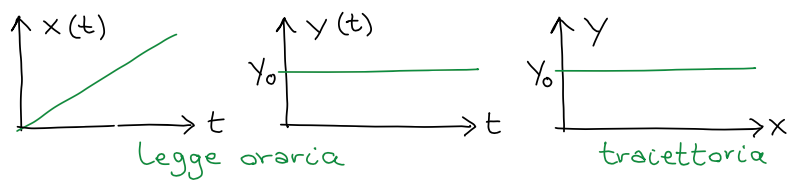
\includegraphics[width=0.8\textwidth]{images/ess-traiettoria.png}
    \end{figure}
\end{example}

\begin{definition}
    La \textbf{velocità istantanea} è la derivata della posizione rispetto al tempo.
    $$v = \lim_{\Delta t \to 0}\frac{\Delta s}{\Delta t} = \frac{ds}{dt}$$
\end{definition}

\begin{definition}
    La \textbf{velocità media} è definita come il rapporto tra lo spostamento e l'intervallo di tempo necessario per effettuarlo.
    $$v_m = \frac{\Delta s}{\Delta t}$$
\end{definition}
\hspace{-15pt}In parole povere è una grandezza che ci dice con quale rapidità cambia la posizione di un punto rispetto al tempo nell'instante $t$.
\subsection*{Vettore velocità}
Derivata rispetto al tempo del vettore posizione e si indica come 
$\frac{d\vec{r}(t)}{dt}\text{ oppure }\dot{\vec{r}}(t)[m/s]$
\begin{equation}
    \begin{split}
    \dot{\vec{r}}(t) & = (\dot{x}(t), \dot{y}(t), \dot{z}(t)) \\
     & = \frac{d}{dt}[x(t)\hat{x} + y(t)\hat{y} + z(t)\hat{z}] \\
     & = \dot{x}(t)\hat{x} + \dot{y}(t)\hat{y} + \dot{z}(t)\hat{z}
    \end{split}
\end{equation}
Per ricavare la forma esplicita uso le proprietà delle derivate (\textbf{linearità}, \textbf{Leibnitz})
\begin{example}
    $\vec{r}(t) = (v_0t, y_0, 0) = v_0t\hat{x} + y_0\hat{y}$ \:\:\:abbiamo che \:\:\:
    $\dot{\vec{r}}(t) = (v_0, 0, 0) = v_0 \hat{x}$
\end{example}
\hspace{-15pt}Velocità e spazio percorso ("integrale di linea").\\
\begin{wrapfigure}[3]{l}{5cm}
    \centering
    \includegraphics[width=5cm]{images/vettore-velocità.png}
\end{wrapfigure}
\begin{align*}
    L & = ||\vec{r}(t_1) - \vec{r}(t_0)|| + ||\vec{r}(t_2) - \vec{r}(t_1)|| + ||\vec{r}(t_3) - \vec{r}(t_2)|| + \dots \\
    & = \sum_i ||\vec{r}(t_{i+1} - \vec{r}(t_i)|| \:\: per\:\: |t_{i+1} - t_i| \text{"piccolo"} \\
    & = \sum_i ||\frac{\vec{r}(t_{i+1}) - \vec{r}(t_i)}{t_{i+1} - t_i}|| (t_{i+1} - t_i) = \int_{t_{in}}^{t_{f_{in}}}||\dot{\vec{r}}(t)||\\
\end{align*}
\begin{example}
    $\vec{r}(t) = (v_0t, y_0)\:\:\: \dot{\vec{r}}(t) = (v_0, 0)$\hspace{15pt}
    $||\dot{\vec{r}}(t)|| = \sqrt{v_0^2 + 0^2} = |v_0|$ \:\:\: $L = |v_0| \cdot (t_{f_{in}} - t_{in})$\\
    Il vettore è costante quindi facendo la derivata torna zero. Con la velocità si calcolo lo spazio percorso ("integrale di linea").
    La differenza fra le posizioni e la differenza dei tempi è il rapporto incrementale in caso gli intervalli siano sufficentemente
    piccoli, da qui si ottiene l'integrale.
\end{example}

\subsection{Vettore accelerazione}
Derivata rispetto al tempo del vettore velocità e si indica con $\frac{d^2\vec{r}(t)}{dt} \text{ oppure } \ddot{\vec{r}}(t) [m/s^2]$
\begin{equation}
    \ddot{\vec{r}}(t) = (\ddot{x}(t), \ddot{y}(t), \ddot{z}(t))\:\: = \:\: \ddot{x}(t)\hat{x} + \ddot{y}(t)\hat{y} + \ddot{z}(t)\hat{z}
\end{equation}
\begin{example}
    $\vec{r}(t)= (\frac{1}{2}a_0t^2, v_0t, 0)$ \hspace{10pt} $\dot{\vec{r}}(t) = (a_0t, v_0, 0)$ \hspace{10pt} $\dot{\vec{r}}(t) = (a_0, 0, 0)$
\end{example}
\hspace{-15pt}Serve perché l'equazione "del moto" di Newton che determinata la legge oraria è formulata in termini di accelerazione.

\subsection{Vettore quantità di moto}
Il prodotto di massa [kg] e velocità [m/s]
$$\vec{p}(t) = m \cdot \dot{\vec{r}}(t) = (m\dot{x}(t), m\dot{y}(t), m\dot{x}(t)) = m\dot{\vec{x}}(t)x + m\dot{\vec{y}}(t)y + m \dot{\vec{z}}(t)z$$
\begin{example}
    Prendiamo un punto di massa 2kg e velocità 3m/s lungo $\hat{x}$.\\
    $p_x(t) = 2 \cdot 3 kg\cdot m/s = 6 kg \cdot m/s$ \hspace{15pt} $p_y(t) = p_z(t) = 0$.
\end{example}
\hspace{-15pt}Serve per generalizzare l'equazione di Newton e per trattare sistemi di piu punti materiali.

\subsection{Vettore momento angolare rispetto a un polo P}
$$\vec{L}_p(t) = m(\vec{r}(t) - \vec{r}_p) \times \dot{\vec{r}}(t)$$
Dove $\vec{r}_p$ è il vettore posizione di p, mentre $\dot{\vec{r}}(t)$ è il prodotto vettoriale.
\begin{example}
    $\vec{r}_p = (l_0, 0, 0)$ \hspace{15pt} $\vec{r}(t) = (v_0t, y_0, 0)$\\
    $\vec{L}_p = m[(v_0t - l_0)\hat{x} + y_0\hat{y}] \times (v_0\hat{x}) \:\: = \:\: m(v_0t - l_0)v_0 \hat{x} \times \hat{x} + my_0v_0\hat{y}\times \hat{x} 
    \:\: = \:\: my_0v_0(-\hat{z}) = (0,0, -my_0v_0)$\\
    Ricorda che $\hat{x} \times \hat{x} = 0$ e $\hat{y} \times \hat{x} = -\hat{z}$
\end{example}
\hspace{-15pt}Il momento angolare dice quanta inerzia ha un oggetto in una rotazione (descrizione sommaria).\\
Il polo P è parte della definizione. È una scelta! Il risultato dipende dal polo.
Serve per formulare l'equazione del moto di sistemi di punti materiali e corpi rigidi.

\subsection{Coordinate polari}
Un metodo per rapprensentare delle cordinate x, y andando a misurare prima la distanza dall'origine e poi si va a vedere
quanto vale l'angolo fra questo segmento dall'asse x, utilizzando seno e coseno.
\begin{wrapfigure}[7]{l}{2cm}
    \centering
    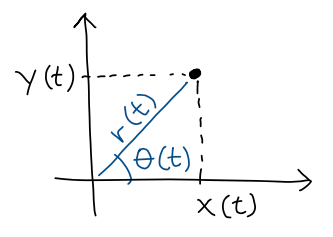
\includegraphics[width=5.5cm]{images/coordinate-polari.png}
\end{wrapfigure}
\begin{align*}
    \begin{cases}
        x(t) = r(t) \cdot \cos(\Theta(t))\\
        y(t) = r(t) \cdot \sin(\Theta(t)) 
    \end{cases}
\end{align*}
\begin{align*}
    \begin{cases}
        r(t) = \sqrt{x(t)^2 + y(t)^2} \geq 0\\
        tg(\Theta(t)) = y(t) / x(t) 
    \end{cases}
\end{align*}
\\
\begin{example} Esempi di rappresentazione di coordinate in coordinate polari.\\
    $x = 0, y = l_0 > 0 \:\: \Rightarrow \:\: r = l_0, \Theta = \pi/2$\\
    $x = 0, y = -l_0 < 0 \:\: \Rightarrow \:\: r = l_0, \Theta = -\pi/2$\\
    $x = l_0, y = l_0 > 0 \:\: \Rightarrow \:\: r = \sqrt{2}l_0, \Theta = \pi/4$\\
\end{example}

\subsection{Versori polari (2D)}
Definisco un versore $\hat{r}(t)$ che punta verso il punto materiale e un versore $\hat{\Theta}(t)$ ortogonale.
Si esprime facilmente in coordinte polari.
$$\vec{r}(t) = (x(t), y(t)) = (r(t)\cos \Theta(t), r(t)\sin\Theta(t)) \:\: = \:\: r(t)(\cos\Theta(t)\hat{x} + \sin\Theta(t)\hat{y})$$
Ma $||\vec{r}(t)|| = |r(t)| = r(t)$ allora definisco $\hat{r}(t) = \vec{r}(t)/ ||\vec{r}(t)|| = \cos \Theta(t)\hat{x} + \sin\Theta(t)\hat{y}$\\\\
Trovo facilmente che un versore ortogonale è:
$$\hat{\Theta(t)} = -\sin\Theta(t)\hat{x} + \cos\Theta(t)\hat{y} \:\:\:\text{infatti} \:\:\: \hat{r}\cdot \hat{\Theta} = c \cdot (-s) + s \cdot c = 0$$
\begin{wrapfigure}[7]{r}{6cm}
    \centering
    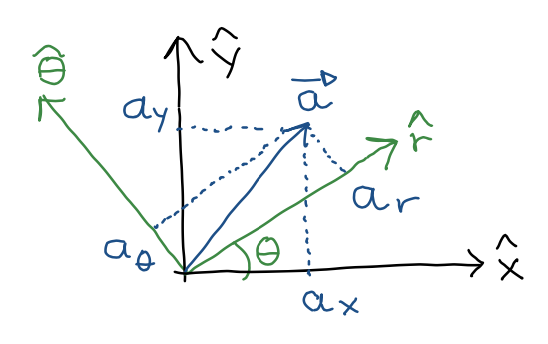
\includegraphics[width=5.5cm]{images/trasformazioni-inverse.png}
\end{wrapfigure}
\begin{note}
    Non c'è legame fra $\Theta$ e $\hat{\Theta}$ è solo una convenzione.
\end{note}
\hspace{-15pt}Le trasformazioni inverse invece si fanno come segue (verifico per sostituzione):
$$\hat{y} = \cos\Theta(t)\hat{r} - \sin\Theta(t)\hat{\Theta} \hspace{20pt} \hat{y} = \sin\Theta(t)\hat{r} + \cos\Theta(t)\hat{\Theta}$$
Possono quindi scrivere ogni vettore nella forma $\vec{a} = a_r\hat{r} + a_{\Theta}\hat{\Theta}$ con le componenti polari $a_r, a_{\Theta}$.
Per evitare ambiguità non scriviamo $(a_r, a_{\Theta})$ e riserviamo la notazione alle componenti cartesiane.\\\\
A differenza dei versori cartesiani quelli polari dipendono dal tempo per costruzioni.
$$\dot{\hat{r}}(t) = \frac{d}{dt}[\cos\Theta(t) \hat{x} + \sin\Theta(t)\hat{y}] \:\: = \:\: -\sin\Theta(t) \cdot \dot{\Theta}(t)\hat{x} + \cos\Theta(t) \cdot \dot{\Theta}(t)\hat{y}$$
Dove $\cos\Theta(t) \cdot \dot{\Theta}(t)$ si applica la derivata della somma, Leibnitz, funzione composta.
$$= \dot{\Theta}(t)\cdot \hat{\Theta}(t) \:\:\:\:(\text{confronto l'espressione di} \hat{\Theta}(t))$$
Similmente $\dot{\hat{\Theta}}(t)= - \dot{\Theta}\hat{r}(t)$.


\subsection*{Vettori posizione, velocità, accelerazione}
$$\vec{r}(t) = r(t)\hat{r}(t)$$
Dove abbiamo che $\vec{r}(t)$ è il vettore, $r(t)$ è una coordinata polare, $\hat{t}(t)$ è il versore polare.
$$\dot{\vec{r}}(r) = \dot{r}(t)\hat{r}(t) + r(t)\dot{\Theta}(t)\hat{\Theta}(t)$$
Dove la parte $\dot{\vec{r}}(r)$ è la velocità radiale.
$$\ddot{\vec{r}}(t) = [\ddot{r}(t) - r(t)\dot{\Theta}(t)^2] \hat{r} + [r(t) \ddot{\Theta}(t) + 2\dot{r}(t)\dot{\Theta}(t)]\hat{\Theta}$$
Nel quale abbiamo che la parte $r(t)\dot{\Theta}(t)^2$ si chiama \textbf{velocità centripeta}, mentre $2\dot{r}(t)\dot{\Theta}(t)$ si dice \textbf{accelerazione di Coriolis}.


	% !TeX spellcheck = it_IT
\newpage
\section{Agenti intelligenti}
L'approccio moderno dell'IA (AIMA) è quello di costruire degli \textbf{agenti intelligenti}. La visione ad agenti offre n quadro di riferimento e una prospettiva più generale. È utile anche perché è \textbf{uniforme}.
\begin{center}
	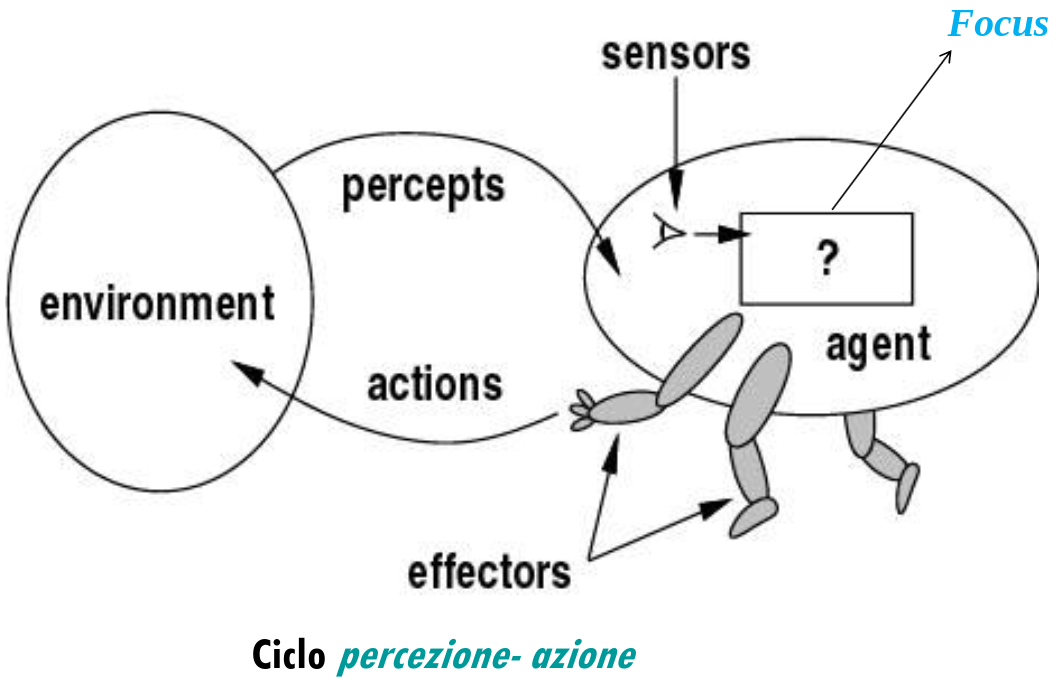
\includegraphics[scale=0.25]{images/agente.png}
\end{center}
Noi ci concentreremo sul programma che sta al centro dell'agente e che consiste in un ciclo di percezione-azione.
\subsection{Caratteristiche}
Un agente ha alcune caratteristiche:
\begin{itemize}
	\item \textbf{Situati}: ricevono \emph{percezioni} da un ambiente e agiscono mediante \textbf{azioni} (attuatori)
	
\end{itemize}

\subsubsection{Percezioni e azioni}
Le percezioni corrispondono agli \textbf{input} dai sensori. La \textbf{sequenza percettiva} sarà la storia completa delle percezioni.\\
La scelta dell'azione è \emph{funzione} unicamente della sequenza percettiva ed è chiamata \textbf{funzione agente}.\\
Il compito dell'IA è costruire il programma agente.
\begin{center}
	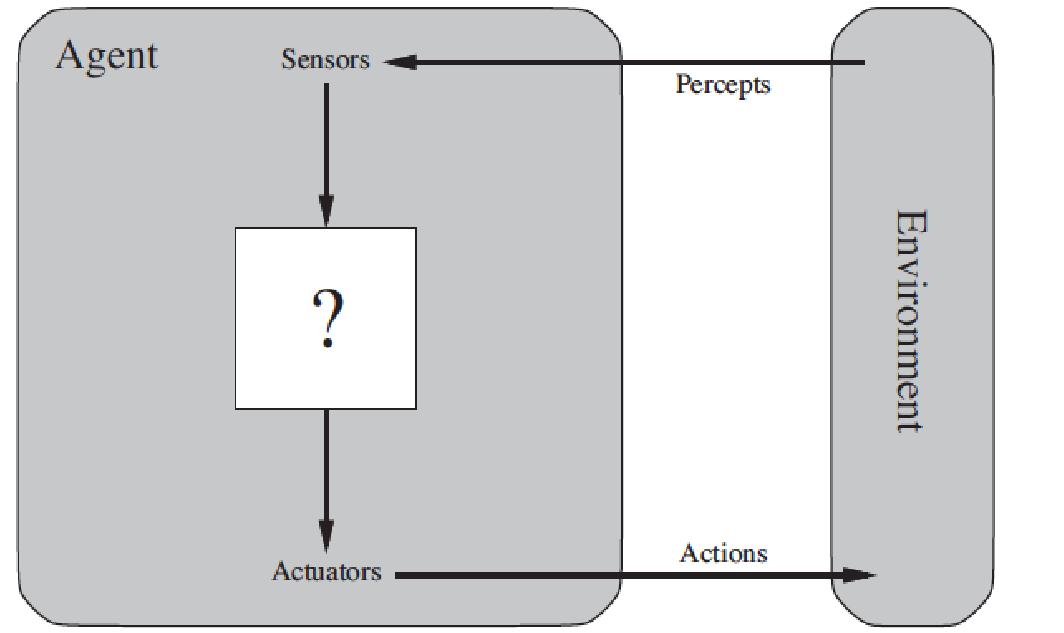
\includegraphics[scale=0.2]{images/architettura_astratta.png}
	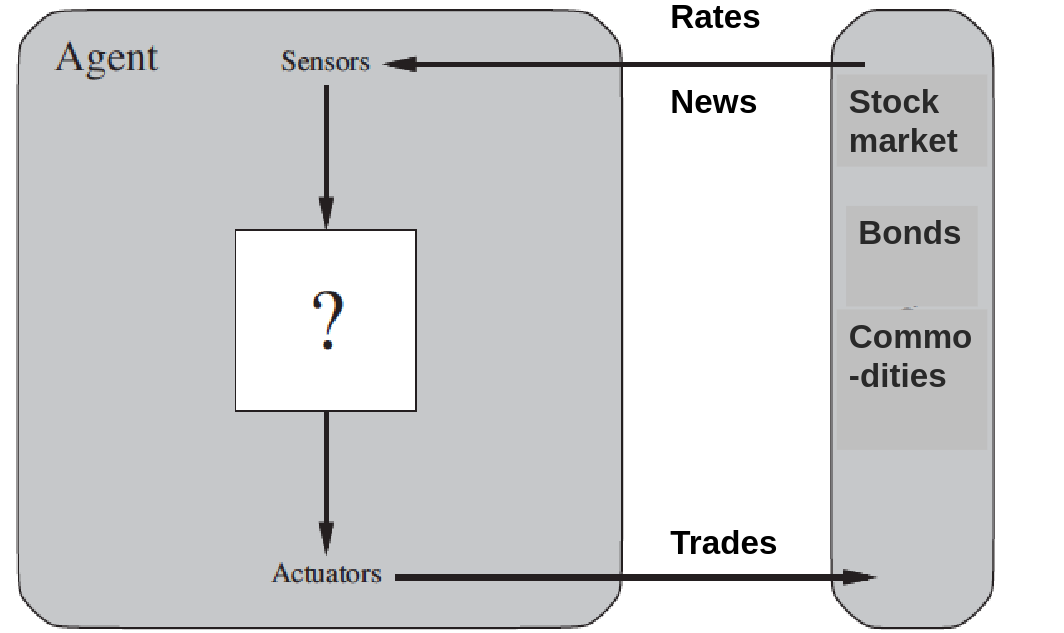
\includegraphics[scale=0.2]{images/agente_finanziario.png}
\end{center}
%TODO Caption

\subsection{Agente razionale}
Un agente razionale interagisce con il suo ambiente in maniera \textbf{efficace} (fa la cosa giusta).
Si rende quindi necessario un \textbf{criterio di valutazione} oggettivo dell'effetto delle azioni dell'agente. La valutazione della prestazione deve avere le seguenti caratteristiche:
\begin{itemize}
	\item Esterna (come vogliamo che il mondo evolva?)
	\item Scelta dal progettista a seconda del problema considerando l'effetto desiderato sull'ambiente.
	\item (possibile) Valutazione su ambienti diversi.
\end{itemize}
\begin{definition}[Agente razionale]
	Per ogni sequenza di percezioni compie l’azione che massimizza il valore atteso della
	misura delle prestazioni, considerando le sue percezioni passate e la sua conoscenza pregressa.
\end{definition}
\begin{observation}
	Si basa sulla razionalità e non sull'onniscenza e onnipotenza: non conosce alla perfezione il futuro ma può apprendere e hai dei limiti nelle sue azioni.
\end{observation}

Raramente tutta la conoscenza sull’ambiente può essere fornita a priori dal programmatore. L’agente razionale deve essere in grado di modificare il proprio comportamento con l’esperienza. Può \textbf{migliorare} esplorando, apprendendo, aumentando l'autonomia per operare in ambienti differenti o mutevoli.

\begin{definition}[Agente autonomo]
	Un agente è autonomo nella misura in cui il suo comportamento dipende dalla sua
	capacità di ottenere esperienza e non dall’aiuto del progettista.
\end{definition}

\subsection{Ambienti}
Definire un problema per un agente significa innanzitutto caratterizzare l'ambiente in cui opera. Viene utilizzata la descrizione \textbf{PEAS}:
\begin{itemize}
	\item \textbf{P}erformance
	\item \textbf{E}nviroment
	\item \textbf{A}ctuators
	\item \textbf{S}ensors
\end{itemize}

\begin{center}
	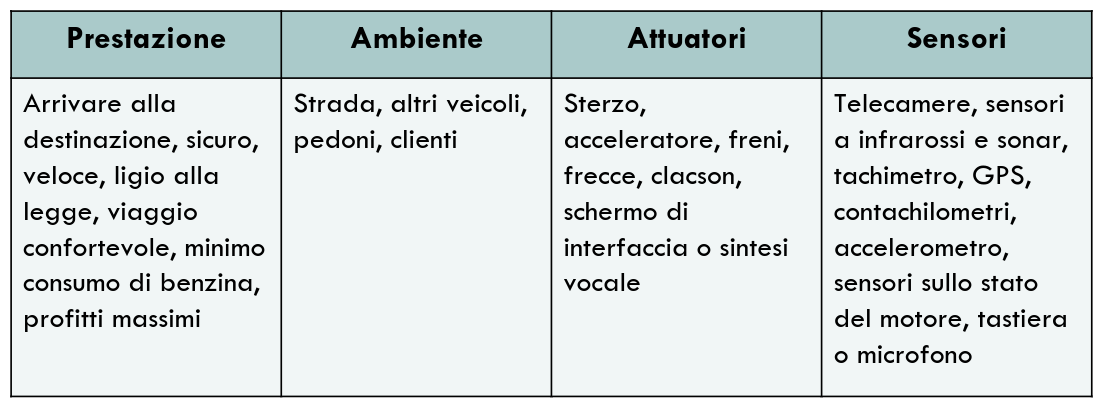
\includegraphics[scale=0.3]{images/agente_ambiente.png}
	%TODO Caption
\end{center}

L'ambiente deve avere le seguenti proprietà:
\begin{itemize}
	\item Osservabilità:
	\begin{itemize}
		\item Se è \textbf{completamente osservabile} l'apparato percettivo è in grado di dare conoscenza completa dell'ambiente o almeno tutto ciò che è necessario per prendere l'azione
		\item Se è \textbf{parzialmente osservabile} sono presenti limiti o inaccuratezze dell'apparato sensoriale
	\end{itemize}
	\item Agente singolo o multi-agente:
	\begin{itemize}
		\item L'ambiente ad agente \textbf{singolo} può anche cambiare per eventi, non
		necessariamente per azioni di agenti
		\item Quello \textbf{multi-agente} può essere \emph{competitivo} (scacchi) o \emph{cooperativo}
	\end{itemize}
	\item Predicibilità:
	\begin{itemize}
		\item \textbf{Deterministico}: quando lo stato successivo è completamente determinato dallo stato corrente e dall’azione (e.g. scacchi)
		\item \textbf{Stocastico}: quando esistono elementi di incertezza con associata probabilità (e.g. guida)
		\item \textbf{Non deterministico}: quando si tiene traccia di più stati possibili risultato dell’azione ma non in base ad una probabilità
	\end{itemize}
\end{itemize}
\newpage
\begin{itemize}
	\item Episodico o sequenziale:
	\begin{itemize}
		\item \textbf{Episodico}: quando l’esperienza dell’agente è divisa in episodi atomici
		indipendenti in cui non c'è bisogno di pianificare (e.g. partite diverse)
		\item \textbf{Sequenziale}: quando ogni decisione influenza le successive (e.g. mosse di scacchi)
	\end{itemize}
	\item Statico o dinamico:
	\begin{itemize}
		\item \textbf{Statico}: il mondo non cambia mentre l’agente decide l’azione (e.g cruciverba)
		\item \textbf{Dinamico}: cambia nel tempo, va osservata la contingenza e tardare equivale a non agire (e.g. taxi)
		\item \textbf{Semi-dinamico}: l’ambiente non cambia ma la valutazione dell’agente sì (e.g. scacchi con timer)
	\end{itemize}
	\item Valori come lo stato, il tempo, le percezioni e le azioni possono assumere valori \textbf{discreti} o \textbf{continui}. Il problema è combinatoriale nel discreto o infinito nel continuo.
	\item \textbf{Noto} o \textbf{ignoto}: una distinzione riferita alla conoscenza dell'agente sulle leggi fisiche dell'ambiente (le regole del gioco). È diverso da osservabile.
\end{itemize}

\begin{definition}[Simulatore]
	Un simulatore è uno strumento software che si occupa di:
	\begin{itemize}
		\item Generare stimoli
		\item Raccogliere le azioni in risposta
		\item Aggiornare lo stato
		\item Attivare altri processi che influenzano l'ambiente
		\item Valutare la prestazione degli agenti (media su più istanze)
	\end{itemize}
	Gli esperimenti su classi di ambienti con condizioni variabili sono essenziali per \textbf{generalizzare}.
\end{definition}

\subsection{Programma agente}
L'agente sarà quindi composto da un'architettura e da un programma. Il programma dell'agente implementa la funzione agente $Ag: Percezioni \to Azioni$. 

\begin{lstlisting}
	function Skeleton-Agent (percept) returns action
		static: memory, agent memory of the world
		memory <- UpdateMemory(memory, percept)
		action <- Choose-Best-Action(memory)
		memory <- UpdateMemory(memory, action)
		return action
\end{lstlisting}

\subsubsection{Tabella}
Un agente basato su tabella esegue una scelta come un accesso ad una tabella che associa un'azione ad ogni possibile sequenza di percezioni.\\
Ha una \textbf{dimensione ingestibile}, è difficile da costruire, non è autonomo ed è di difficile aggiornamento (apprendimento complesso).

\subsubsection{Agenti reattivi}
L'agente agisce in base a quello che percepisce senza salvare nulla in memoria.
\begin{center}
	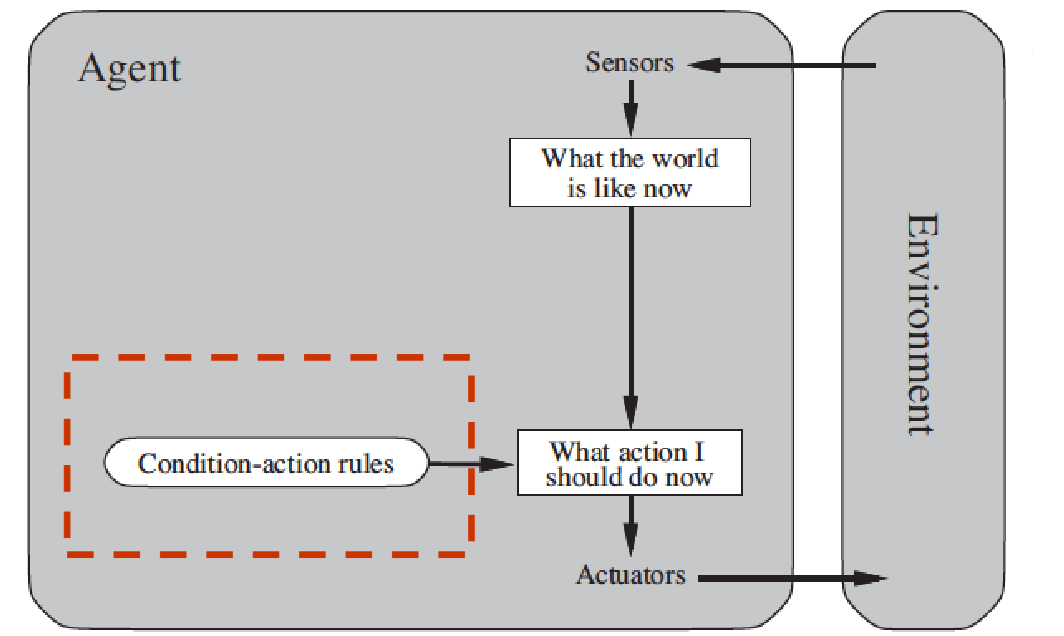
\includegraphics[scale=0.25]{images/agenti_reattivi.png}
\end{center}
\begin{lstlisting}
	function Agente-Reattivo-Semplice (percezione)
		returns azione
		persistent: regole, un insieme di regole
		condizione-azione (if-then)
		stato <- Interpreta-Input(percezione)
		regola <- Regola-Corrispondente(stato, regole)
		azione <- regola.Azione
		return azione
\end{lstlisting}

\subsubsection{Agenti basati su modello}
L'agente ha uno stato che mantiene la storia delle percezioni e influenza il modello del mondo.
\begin{center}
	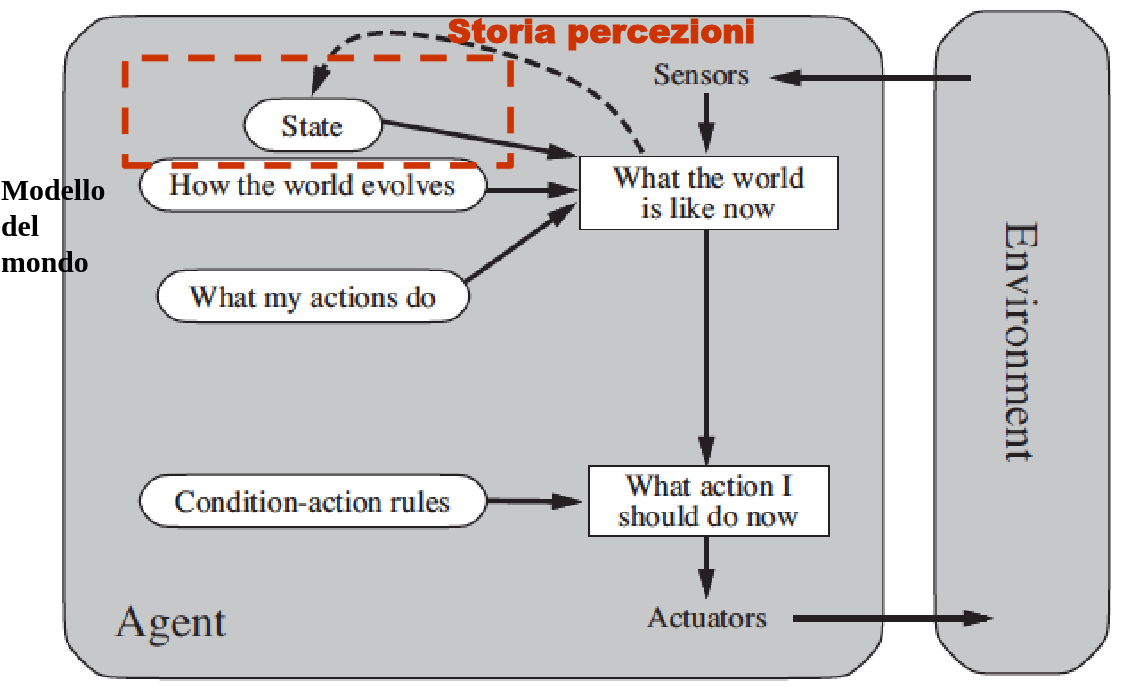
\includegraphics[scale=0.25]{images/agenti_modello.png}
\end{center}
\begin{lstlisting}
	function Agente-Basato-su-Modello (percezione)
		returns azione
		persistent: stato, una descrizione dello stato corrente
								modello, conoscenza del mondo
								regole, un insieme di regole condizione-azione
								azione, azione piu recente
		stato <- Aggiorna-Stato(stato, azione, percez., modello)
		regola <- Regola-Corrispondente(stato, regole)
		azione <- regola.Azione
		return azione
\end{lstlisting}

\subsubsection{Agenti con obiettivo}
Fin'ora l'agente aveva un obiettivo predeterminato dal programma. In questo caso invece viene specificato anche il \textbf{goal} che influenza le azioni. Abbiamo quindi più \textbf{flessibilità} ma meno efficienza.
\begin{center}
	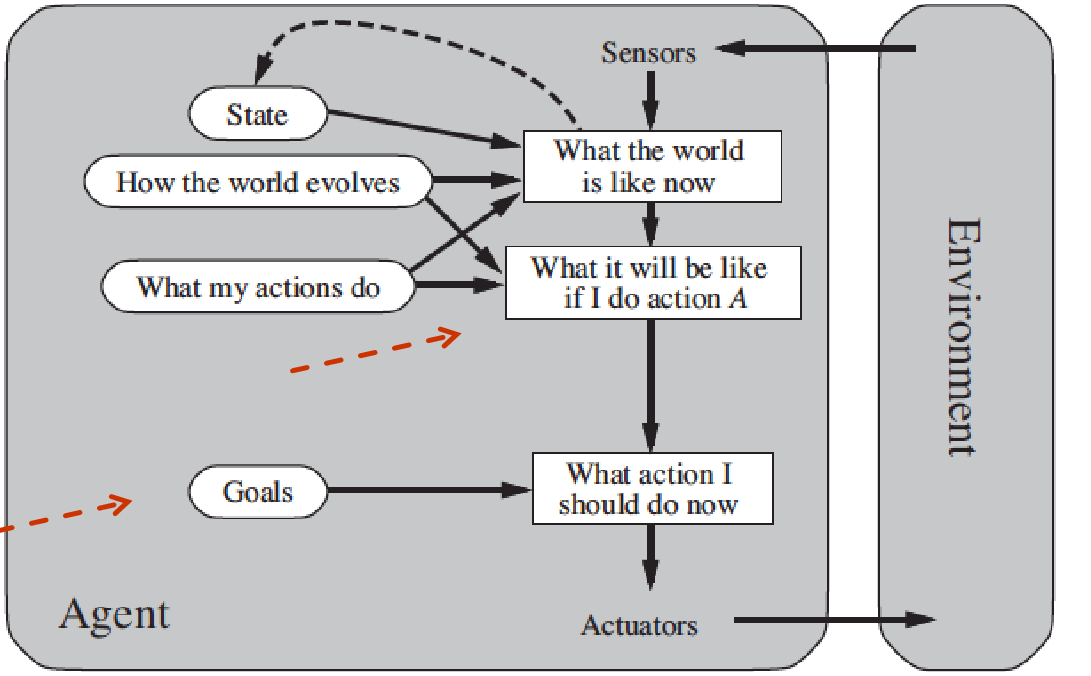
\includegraphics[scale=0.25]{images/agenti_obiettivo.png}
\end{center}

\subsubsection{Agenti con valutazione di utilità}
In questo caso ci sono \textbf{obiettivi alternativi} o più modi per raggiungerlo. L'agente deve quindi decidere verso dove muoversi e si rende necessaria una \textbf{funzione utilità} che associ ad un obiettivo un numero reale. La funzione terrà anche conto della probabilità di successo (\textbf{utilità attesa}).
\begin{center}
	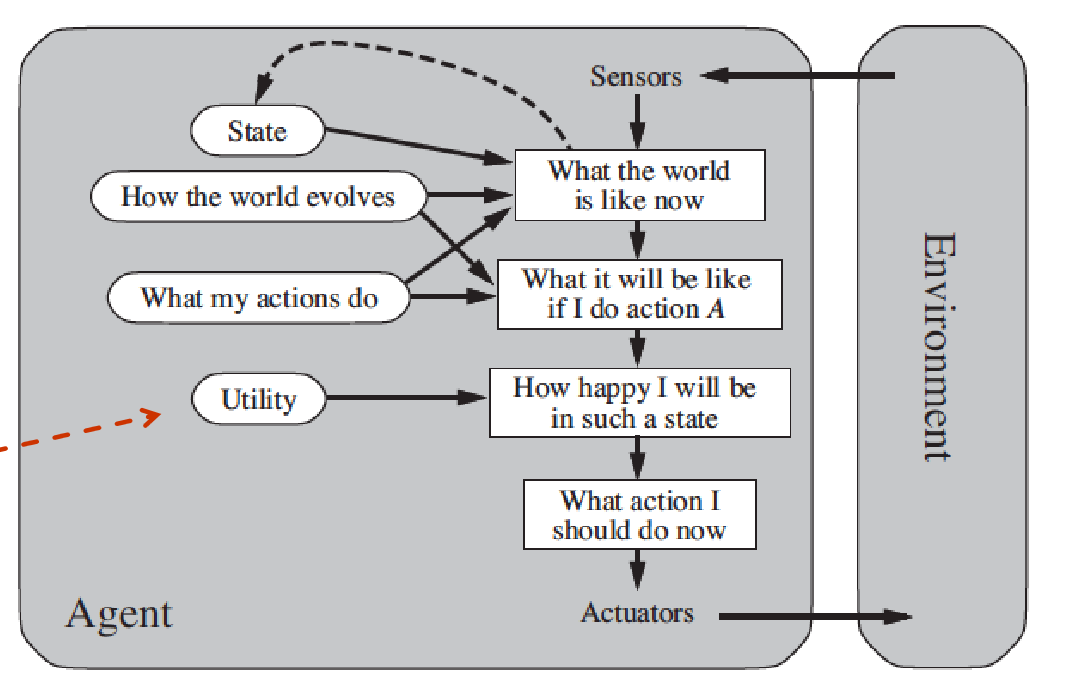
\includegraphics[scale=0.25]{images/agenti_utilita.png}
\end{center}

\subsubsection{Agenti che apprendono}
Questo tipo di agente include la capacità di \textbf{apprendimento} che produce cambiamenti al programma e ne migliora le prestazioni, adattando i comportamenti.\\
L'elemento \textbf{esecutivo} è il programma stesso, quello \textbf{critico} osserva e dà feedback ed infine c'è un generatore di problemi per suggerire nuove situazioni da esplorare.
\begin{center}
	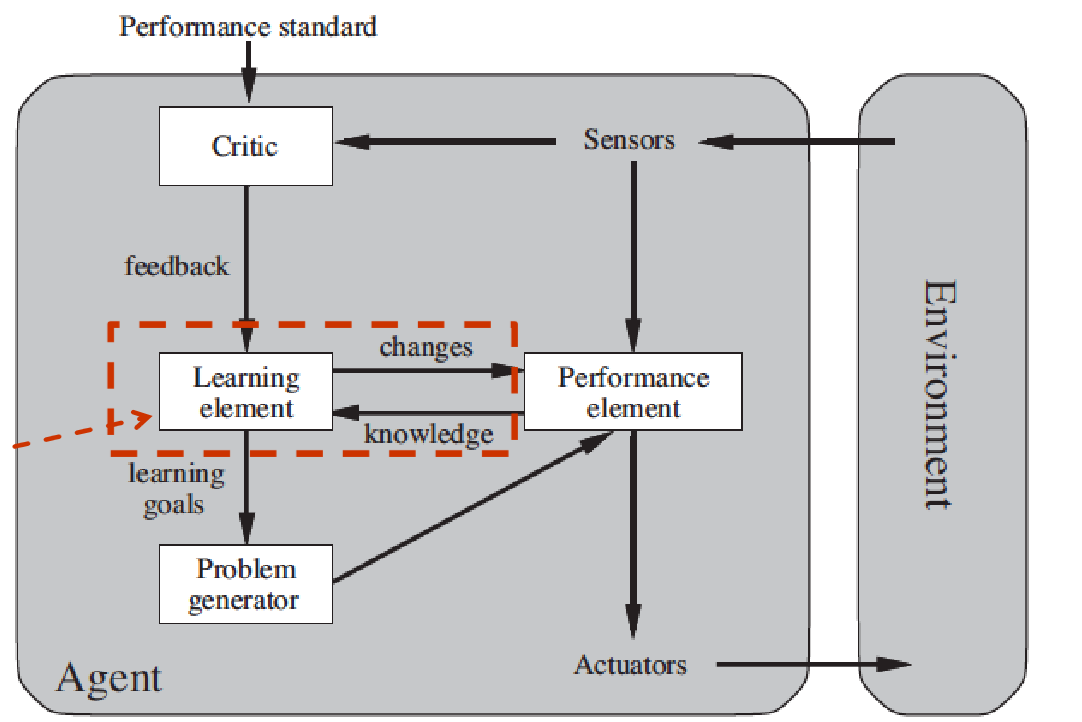
\includegraphics[scale=0.25]{images/agenti_apprendono.png}
\end{center}

\subsubsection{Tipi di rappresentazione}
Gli stati e le transizioni possono essere rappresentati in tre modi:
\begin{itemize}
	\item \textbf{Atomica}: solo con gli stati
	\item \textbf{Fattorizzata}: con più variabili e attributi
	\item \textbf{Strutturata}: con l'aggiunta delle relazioni
\end{itemize}
\begin{center}
	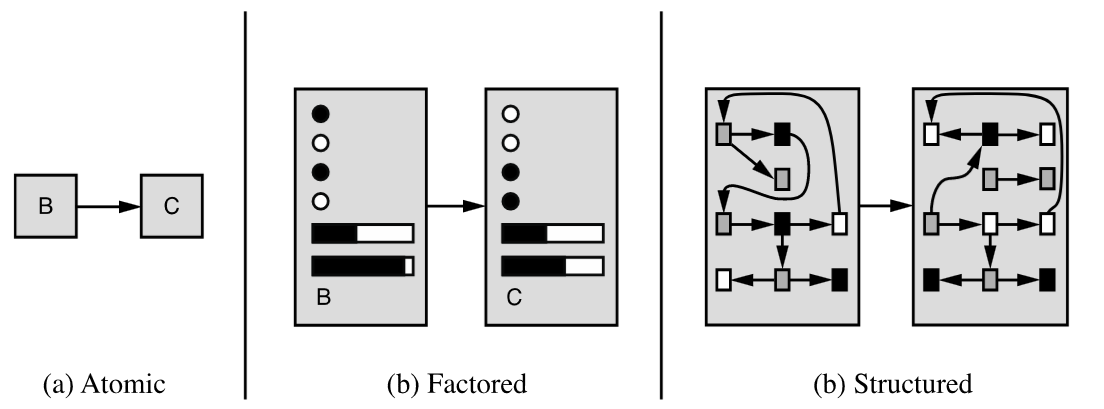
\includegraphics[scale=0.35]{images/rappresentazioni.png}
\end{center}
	% !TeX spellcheck = it_IT
\newpage
\section{Agenti risolutori di problemi}
Gli agenti risolutori di problemi adottano il paradigma della risoluzione di problemi come \textbf{ricerca} in uno \textbf{spazio di stati}. Sono agenti con \textbf{modello} (storia percezioni e stati) che adottano una rappresentazione \textbf{atomica} degli stati.\\
Sono particolari gli agenti con \textbf{obiettivo} che pianificano l'intera sequenza di mosse prima di agire.

\subsection{Processo di risoluzione}
I passi da seguire sono i seguenti:
\begin{enumerate}
	\item \textbf{Determinazione di un obiettivo}, ovvero un insieme di stati in cui l'obiettivo è soddisfatto
	\item \textbf{Formulazione} del problema tramite la rappresentazione degli stati e delle azioni
	\item Determinazione della \textbf{soluzione} mediante la ricerca
	\item \textbf{Esecuzione} del piano
\end{enumerate}

\begin{example}[Viaggio con mappa]
	Supponiamo di voler fare un viaggio. Il processo di risoluzione sarebbe il seguente:
	\begin{enumerate}
		\item Raggiungere Bucarest
		\item \begin{itemize}
			\item Azioni: guidare da una città all'altra
			\item Stato: città su mappa
		\end{itemize}
	\end{enumerate}
\end{example}

\subsection{Assunzioni}
Assumiamo che l'ambiente in questione sia \textbf{statico}, \textbf{osservabile}, \textbf{discreto} e \textbf{deterministico} (assumiamo un mondo ideale).

\subsection{Formulazione del problema}
Un problema può essere definito formalmente mediante 5 componenti:
\begin{enumerate}
	\item \textbf{Stato iniziale}
	\item \textbf{Azioni} possibili
	\item \textbf{Modello di transizione}: $ris: stato \times azione \to stato$, uno stato \emph{successore} $ris(s,a)=s'$
	\item \textbf{Test obiettivo} per capire tramite un insieme di stati obiettivo se il goal è raggiunto $test: stato \to \{true,false\}$
	\item \textbf{Costo del cammino}: composto dalla somma dei costi delle azioni, dove un passo ha costo $c(s,a,s')$. Un passo non ha mai costo negativo.
\end{enumerate}
I punti 1, 2 e 3 definiscono implicitamente lo \textbf{spazio degli stati}. Definirlo esplicitamente può essere molto costoso.

\subsection{Algoritmo di ricerca}
Gli algoritmi di ricerca prendono in input un problema e restituiscono un \textbf{cammino soluzione}.\\
Dobbiamo misurare le \textbf{prestazioni}: trova una soluzione? Quanto costa trovarla? Quanto è efficiente?
\begin{equation*}
	costo\_totale=costo\_ricerca+costo\_cammino\_sol
\end{equation*}

\begin{example}[Arrivare a Bucarest]
	Partiamo con la formulazione del problema:
	\begin{enumerate}
		\item \textbf{Stato iniziale}: la città di partenza, ovvero Arad
		\item \textbf{Azioni}: spostarsi in una città collegata vicina
		\begin{lstlisting}
			Azioni(In(Arad))={Go(Sibiu),Go(Zerind),...}
		\end{lstlisting}
		\item \textbf{Modello di transizione}: 
		\begin{lstlisting}
			Risultato(In(Arad), Go(Sibiu)) = In(Sibiu)
		\end{lstlisting}
		\item \textbf{Test obiettivo}:
		\begin{lstlisting}
			{In(Bucarest)}
		\end{lstlisting}
		\item \textbf{Costo del cammino}: somma delle lunghezze delle strade
	\end{enumerate}
	In questo esempio lo spazio degli stati coincide con la rete dei collegamenti tra le città.
	\begin{center}
		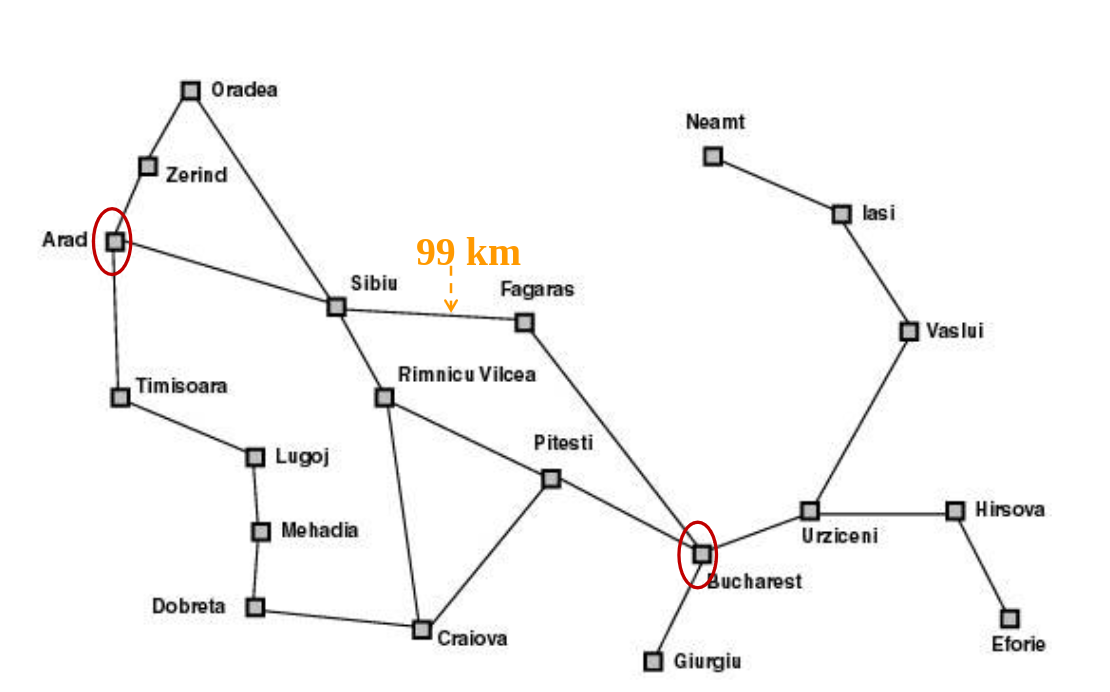
\includegraphics[scale=0.2]{bucarest_example.png}
	\end{center}
\end{example}

\begin{example}[Puzzle dell'8]
	Partiamo con la formulazione del problema:
	\begin{enumerate}
		\item \textbf{Stati}: tutte le possibili configurazioni della scacchiera
		\item \textbf{Stato iniziale}: una configurazione tra quelle possibili
		\item \textbf{Obiettivo}: una configurazione del tipo
		\begin{center}
			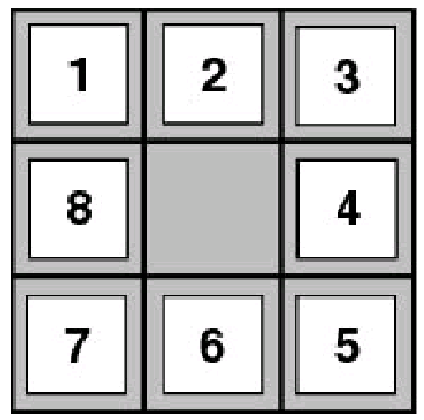
\includegraphics[scale=0.2]{8_puzzle_win.png}
		\end{center}
		\item \textbf{Azioni}: le mosse della casella vuota
		\item \textbf{Costo cammino}: ogni passo costa 1
	\end{enumerate}
	In questo esempio lo spazio degli stati è un grafo con possibili cicli (ci possiamo ritrovare in configurazioni già viste). Il problema è NP-completo: per 8 tasselli ci sono $\frac{9!}{2}=181.000$ stati.
\end{example}

\begin{example}[8 regine]
	Supponiamo di dover collocare 8 regine su una scacchiera in modo tale che nessuna regina sia attaccata da altre.
	\begin{enumerate}
		\item \textbf{Stati}: tutte le possibili configurazioni della scacchiera con 0-8 regine
		\item \textbf{Goal test}: avere 8 regine sulla scacchiera, di cui nessuna è attaccata
		\item \textbf{Azioni}: aggiungi una regina
	\end{enumerate}
	In questo esempio lo spazio degli stati sono le possibili scacchiere, ovvero $64 \times 63 \times \ldots \times 57 \simeq 1.8 \times 10^{14}$.\\
	Proviamo ad utilizzare una formulazione diversa:
	\begin{enumerate}
		\item \textbf{Stati}: tutte le possibili configurazioni della scacchiera in cui \emph{nessuna regina è minacciata}
		\item \textbf{Goal test}: avere 8 regine sulla scacchiera, di cui nessuna è attaccata
		\item \textbf{Azioni}: aggiungere una regina nella colonna vuota più a destra ancora libera in modo che non sia minacciata
	\end{enumerate}
	Lo spazio degli stati passa a $2057$, anche se comunque rimane esponenziale per $k$ regine.\\
	Vediamo infine un'ultima formulazione:
	\begin{enumerate}
		\item \textbf{Stati}: scacchiere con 8 regine, una per colonna
		\item \textbf{Goal test}: nessuna delle regine già presenti è attaccata
		\item \textbf{Azioni}: sposta una regina nella colonna se minacciata
		\item \textbf{Costo cammino}: zero
	\end{enumerate}
	Qui lo spazio degli stati è di qualche decina di milione.\\
	Capiamo quindi che formulazioni diverse del problema portano a spazi di stati di dimensioni diverse.
\end{example}

\begin{example}[Dimostrazione di teoremi]
	Dato un insieme di premesse:
	\begin{equation}
		\{s, t, q \Rightarrow p, r \Rightarrow p, v \Rightarrow q, t \Rightarrow r, s \Rightarrow v\}
	\end{equation}
	dimostrare una proposizione $p$ utilizzando solamente la regola di inferenza \emph{Modus Ponens}:
	\begin{equation*}
		(p \wedge p\Rightarrow q) \Rightarrow q
	\end{equation*}
	Scriviamo la formulazione del problema:
	\begin{itemize}
		\item \textbf{Stati}: insieme di proposizioni
		\item \textbf{Stato iniziale}: le premesse
		\item \textbf{Stato obiettivo}: un insieme di proposizioni contenente il teorema da dimostrare
		\item \textbf{Operatori}: l'applicazione del Modus Ponens
	\end{itemize}
	Lo spazio degli stati è quindi il seguente:
	\begin{center}
		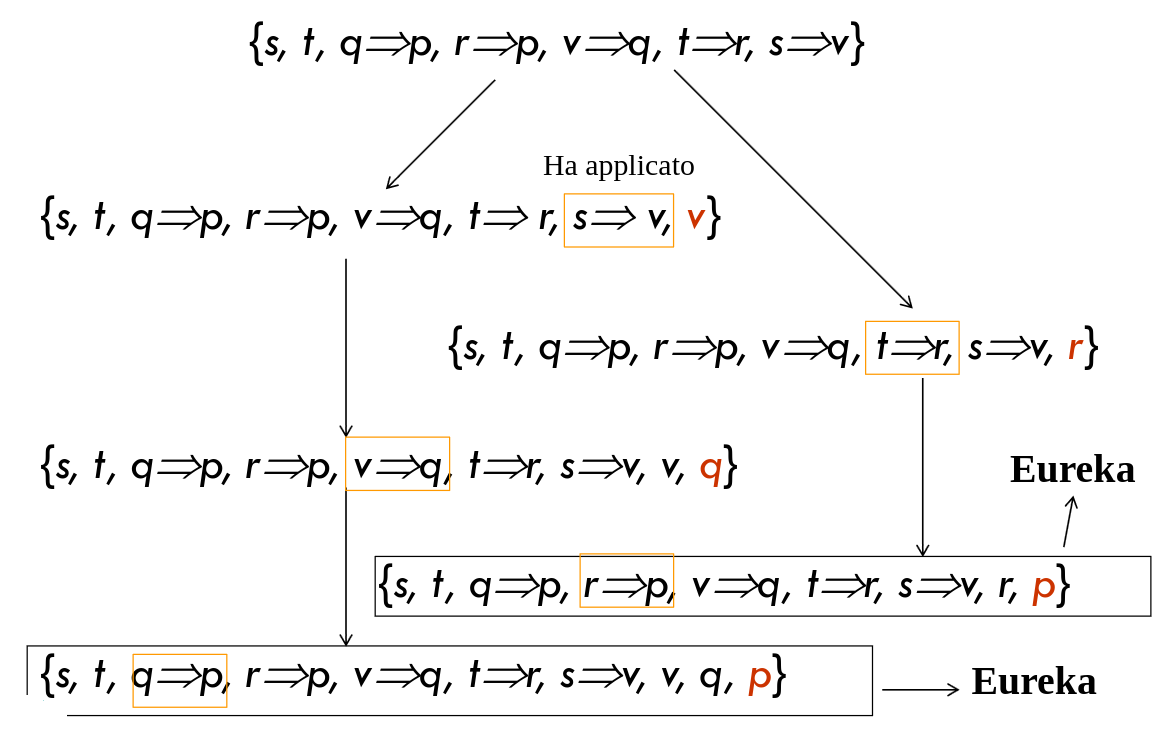
\includegraphics[scale=0.3]{dimostrazione_teoremi.png}
	\end{center}
\end{example}

%TODO Spostare da qui in poi in un altro file
\subsection{Ricerca della soluzione}
La ricerca della soluzione consiste nella generazione di un \textbf{albero di ricerca} a partire dalle possibili sequenze di azioni che si sovrappone allo spazio degli stati.\\
Ad esempio per il caso di Bucarest:
\begin{center}
	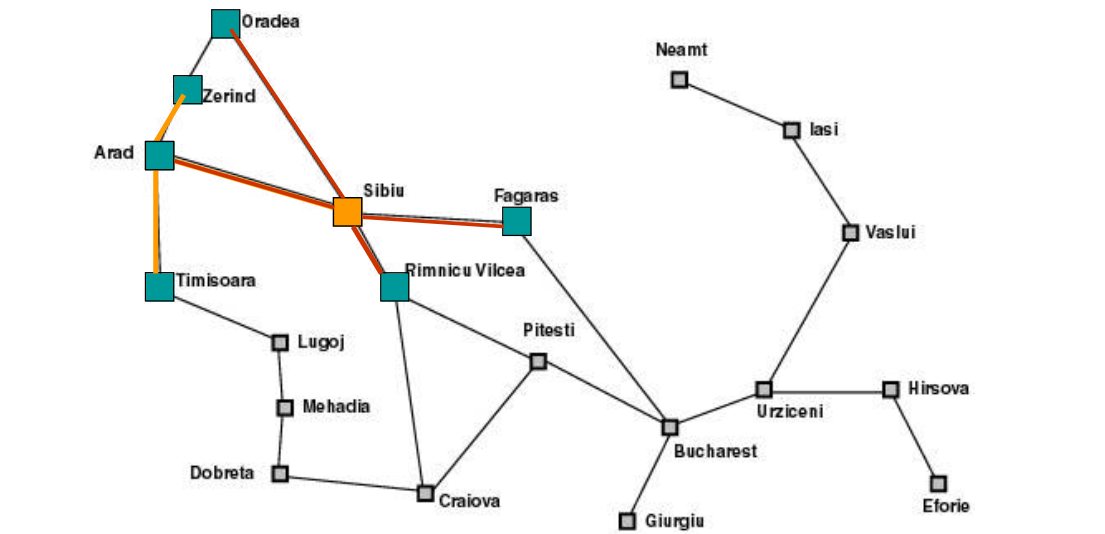
\includegraphics[scale=0.3]{bucarest_tree.png}
\end{center}
Espandiamo ogni nodo con i suoi possibili successori (frontiera).
\begin{definition}[Frontiera]
	Lista dei nodi in attesa di essere espansi (le foglie dell'albero di ricerca).
\end{definition}
\begin{observation}
	Si noti che un nodo dell'albero è diverso da uno stato. Infatti possono esitere nodi dell'albero di ricerca con lo stesso stato (si può tornare indietro).
\end{observation}

\subsection{Strategie di ricerca}
Ci sono diversi tipi di strategia per la ricerca della soluzione:
\begin{itemize}
	\item \textbf{FIFO}
	\item \textbf{LIFO}
	\item \textbf{Coda con priorità}
\end{itemize}

%TODO Ti sei perso delle slide

\subsubsection{Breadth First}
Come esplorare il grafo dello spazio degli stati a livelli progressivi di stessa profondità.\\
Per ogni nodo lo espandiamo, analizziamo i suoi figli (senza scendere ulteriormente di livello) e dopo averli fatti tutti scende di livello seguendo il principio FIFO.\\
Il seguente è il codice della \textbf{ricerca ad albero}, ovvero dove non si torna su un nodo già visitato.

\begin{lstlisting}
	function Ricerca-Ampiezza-A
		returns soluzione oppure fallimento
		nodo = un nodo con stato il problema.stato-iniziale e costo-di-cammino=0
		if problema.Test-Obiettivo(nodo.Stato) then return Soluzione(nodo)
		frontiera = una coda FIFO con nodo come unico elemento
	loop do
		if Vuota?(frontiera) then return fallimento
		nodo = POP(frontiera)
		for each azione in problema.Azioni(nodo.Stato) do
		figlio = Nodo-Figlio(problema, nodo, azione) [costruttore: vedi AIMA]
		if Problema.TestObiettivo(figlio.Stato) then return Soluzione(figlio)
		frontiera = Inserisci(figlio, frontiera) /* frontiera gestita come coda FIFO
	end
\end{lstlisting}

Il seguente è invece quello della \textbf{ricerca su grafo}:
\begin{lstlisting}
	function Ricerca-Ampiezza-g
		returns soluzione oppure fallimento
		nodo = un nodo con stato il problema.stato-iniziale e costo-di-cammino=0
		if problema.Test-Obiettivo(nodo.Stato) then return Soluzione(nodo)
		frontiera = una coda FIFO con nodo come unico elemento
		esplorati = insieme vuoto
	loop do
		if Vuota?(frontiera) then return fallimento
		nodo = POP(frontiera); aggiungi nodo.Stato a esplorati
		for each azione in problema.Azioni(nodo.Stato) do
		figlio = Nodo-Figlio(problema, nodo, azione)
		if figlio.Stato non e in esplorati e non in frontiera then
		if Problema.TestObiettivo(figlio.Stato) then return Soluzione(figlio)
		frontiera = Inserisci(figlio, frontiera) /* in coda
	end
\end{lstlisting}

\noindent Analizziamone la complessità partendo dalle seguenti assunzioni:
\begin{itemize}
	\item Fattore di \textbf{branching} $b$: numero massimo di successori
	\item \textbf{Depth} del nodo obiettivo più superficiale
	\item Lunghezza \textbf{massima} dei cammini nello spazio degli stati
\end{itemize}
La strategia è ottimale se tutti gli operatori hanno lo stesso costo $k$, ovvero se $g(n)=k \cdot depth(n)$, dove $g(n)$ è il costo del cammino per arrivare ad $n$.\\
La complessità nel \emph{tempo} (nodi generati) sarà 
\begin{equation*}
	T(b,d)=1+b+b^2+\ldots+b^d \longrightarrow O(b^d)
\end{equation*}
mentre in \emph{spazio} (nodi in memoria):
\begin{equation*}
	O(b^d)
\end{equation*}
È chiaro che l'algoritmo scali male, sopratutto per quanto riguarda lo spazio.

\subsubsection{Depth first}
In questo algoritmo si parte da un nodo e si scende nel primo figlio, procedendo appunto in profondità. Arrivati alle foglie si torna indietro ai figli precedentemente non visitati. In memoria tengo solamente  i fratelli del path corrente ed elimino i rami già esplorati.\\  Possono esserci tre versioni possibili:
\begin{itemize}
	\item \textbf{Albero}: data $m$ la lunghezza massima dei cammini nello spazio degli stati e $b$ il fattore di diramazione, la \textbf{complessità} in \emph{tempo} è $O(b^m)$ (può essere maggiore di $O(b^d)$) mentre in \emph{spazio} è $b \cdot m$.
	Rispetto al Breadth First, non è né completo né ottimale, ma ci garantisce un notevole risparmio in memoria
	\item \textbf{Grafo}: la memoria corrisponde a tutti i possibili stati, diventando quindi completo nello spazio finito (non in quello infinito)
	\item \textbf{Ricorsiva}: ancora più efficiente per la memoria perché mantiene solo il cammino corrente ($O(m)$). Viene realizzata con un algoritmo di \emph{backtracing} che salva lo stato su uno stack a cui torna in caso di fallimento.
\end{itemize}
\newpage
\begin{lstlisting}
	function Ricerca-DF-A (problema)
		returns soluzione oppure fallimento
		return Ricerca-DF-ricorsiva(CreaNodo(problema.Stato-iniziale), problema)
	
	function Ricerca-DF-ricorsiva(nodo, problema)
		returns soluzione oppure fallimento
		if problema.TestObiettivo(nodo.Stato) then return Soluzione(nodo)
		else
		for each azione in problema.Azioni(nodo.Stato) do
			figlio = Nodo-Figlio(problema, nodo, azione)
			risultato = Ricerca-DF-ricorsiva(figlio, problema)
			if risultato != fallimento then return risultato
		return fallimento
\end{lstlisting}
\subsubsection{Depth Limited}
La ricerca in profondità limitata arriva fino ad un dato livello $l$. È completa solo se si conosce il limite superiore $d$ per la profondità della soluzione e $d<l$. Non è ottimale e ha complessità in tempo $O(b^l)$ e in spazio $O(b \cdot l)$
\subsubsection{Iterative Depth}
Questo approccio prevede di provare l'algoritmo depth limited con limite di profondità $l=0, 1, \ldots$ fino a trovare la soluzione. È il miglior compromesso tra breadth first e depth first:
\begin{itemize}
	\item Complessità in \textbf{tempo} $O(b^d)$ se ammette soluzione
	\item Complessità in \textbf{spazio} $O(b \cdot d)$ se ammette soluzione
\end{itemize}
Quindi ha la \emph{completezza} e l'\emph{ottimalità} del breadth first e la complessità in \emph{spazio} della depth first.
\subsubsection{Uniform Cost}
Partendo da una ricerca in ampiezza, la generalizziamo: si sceglie il nodo di costo minore sulla frontiera e si espande sui contorni di costo uguale.
\begin{center}
	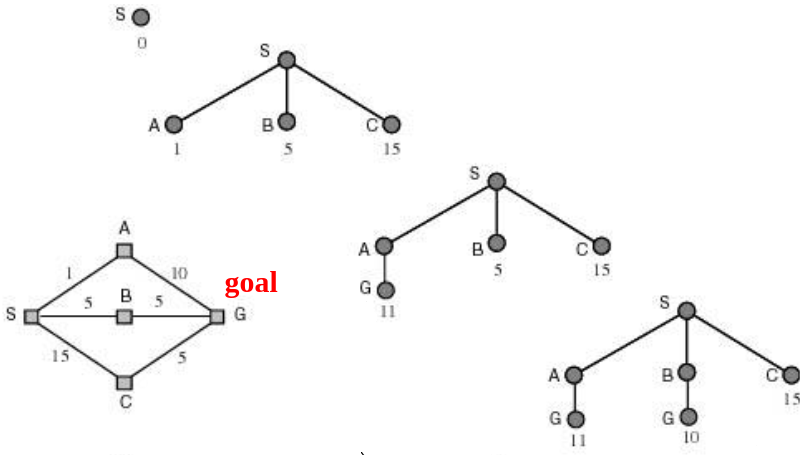
\includegraphics[scale=0.4]{uc.png}
\end{center}
\newpage
Codice per la ricerca su albero:
\begin{lstlisting}
	function Ricerca-UC-A (problema)
			returns soluzione oppure fallimento
			nodo = un nodo con stato il problema.stato-iniziale e costo-di-cammino=0
			frontiera = una coda con priorita con nodo come unico elemento
		loop do
			if Vuota?(frontiera) then return fallimento
			nodo = POP(frontiera)
			if problema.TestObiettivo(nodo.Stato) then return Soluzione(nodo)
			for each azione in problema.Azioni(nodo.Stato) do
				figlio = Nodo-Figlio(problema, nodo, azione)
				frontiera = Inserisci(figlio, frontiera) /* in coda con priorita*/
	end
\end{lstlisting}
Codice per la ricerca su grafo:
\begin{lstlisting}
	function Ricerca-UC-G (problema)
			returns soluzione oppure fallimento
			nodo = un nodo con stato il problema.stato-iniziale e costo-di-cammino=0
			frontiera = una coda con priorita con nodo come unico elemento
			esplorati = insieme vuoto
		loop do
			if Vuota?(frontiera) then return fallimento
			nodo = POP(frontiera);
			if problema.TestObiettivo(nodo.Stato) then return Soluzione(nodo)
			aggiungi nodo.Stato a esplorati
			for each azione in problema.Azioni(nodo.Stato) do
				figlio = Nodo-Figlio(problema, nodo, azione)
				if figlio.Stato non in esplorati e non in frontiera then
					frontiera = Inserisci(figlio, frontiera) /* in coda con priorita
				else if figlio.Stato in frontiera con Costo-cammino piu alto then
					sostituisci quel nodo frontiera con figlio */
	end
\end{lstlisting}
Questo algoritmo è \textbf{ottimo} e \textbf{completo} purché il costo degli archi sia $\epsilon > 0$. Assunto $C^*$ come costo della soluzione ottima, $\lfloor \frac{C^*}{\epsilon}\rfloor$ è il numero di mosse nel caso peggiore. La complessità è quindi $O(b^{1+\lfloor \frac{C^*}{\epsilon}\rfloor})$.
\begin{note}
	Quando ogni azione ha lo stesso costo, la complessità si avvicina a quella della breadth first: $O(b^{1+d})$.
\end{note}
\subsection{Direzione}
Un problema importante è quello della \textbf{direzione} della ricerca, che può essere:
\begin{itemize}
	\item In \textbf{avanti} o guidata da \emph{dati}: si esplora lo spazio di ricerca dallo stato iniziale all'obiettivo
	\item All'\textbf{indietro} o guidata dall'\emph{obiettivo}: si esplora lo spazio di ricerca partendo da uno stato goal e riconducendosi ad un sotto-goal fino a trovare uno stato iniziale
\end{itemize}
Per scegliere la direzione bisogna tenere in conto di quale ha il \textbf{fattore di diramazione} minore.  Si preferisce la ricerca all'\emph{indietro} quando l'obiettivo è ben definito (e.g. theorem proving) mentre quella in \emph{avanti} quando ci sono molteplici obiettivi (e.g. design).\\
\subsubsection{Ricerca bidirezionale}
Nella ricerca bidirezionale si procede in entrambe le direzioni fino ad incontrarsi. La \textbf{complessità} è:
\begin{itemize}
	\item \emph{Tempo}: $O(\sqrt{b^d})$ assumendo che il test dell'intersezione delle due direzioni sia costante
	\item \emph{Spazio}: $O(\sqrt{b^d})$, poiché almeno tutti i nodi di una direzione saranno in memoria
\end{itemize}
Si noti che non sempre è applicabile, come nel caso in cui i predecessori non siano definiti o ci siano troppi stati obiettivo.

\subsection{Problematiche}
\subsubsection{Cicli}
I cammini ciclici rendono gli alberi di ricerca \emph{infiniti} anche quando lo spazio degli stati è finito.
\begin{center}
	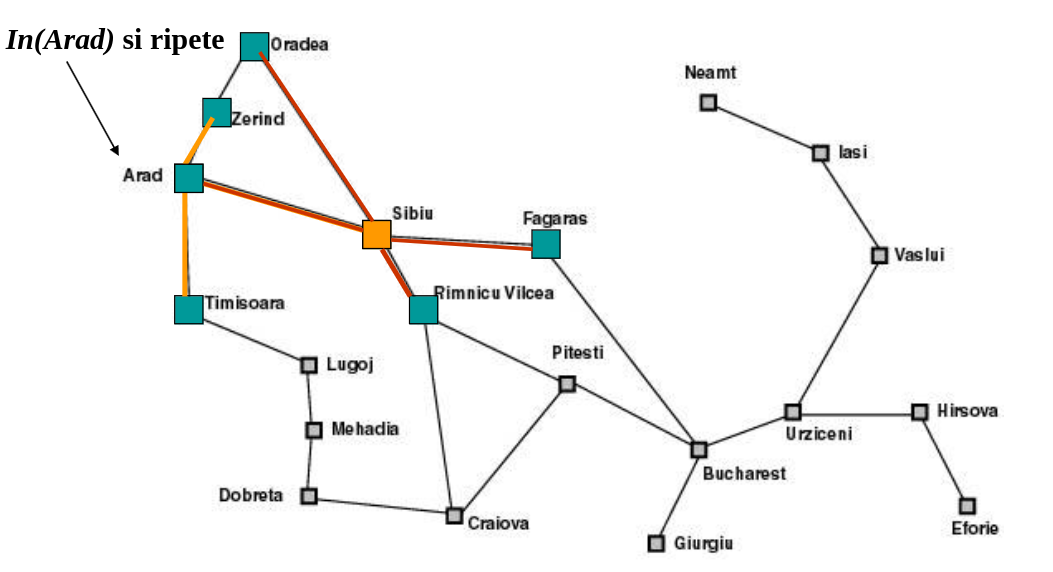
\includegraphics[scale=0.4]{cicli.png}
\end{center}
\subsubsection{Ridondanze}
Su spazi di stati a grafo si possono generare più volte nodi con lo stesso stato nella ricerca, anche in assenza di cicli.
\begin{center}
	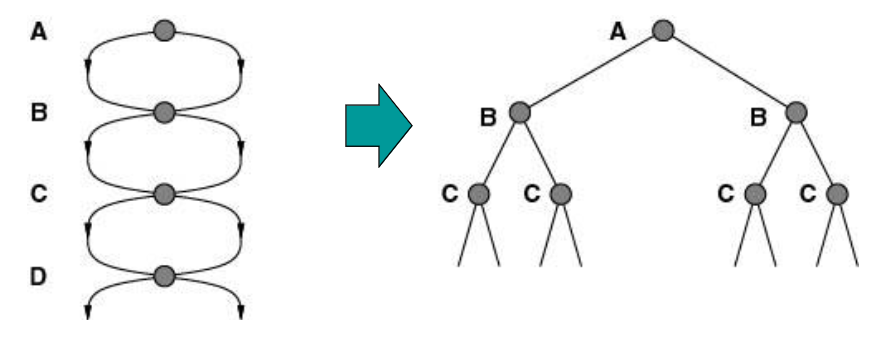
\includegraphics[scale=0.4]{ridondanze.png}
\end{center}
Visitare questi stati è lavoro inutile. Per evitarlo serve \textbf{ricordare} gli stati già visitati, occupando ovviamente più spazio. Tre possibili soluzioni sono:
\begin{enumerate}
	\item Non tornare nel nodo \textbf{genitore}, eliminandolo dai successori (non evita i cammini ridondanti)
	\item Per evitare i \textbf{cammini ciclici} si controlla che  i successori non siano antenati del nodo corrente
	\item Non generare nodi con \textbf{stati già esplorati}: ogni nodo visitato deve essere salvato in memoria
\end{enumerate}
Il costo può essere alto, ad esempio nella depth first la complessità in spazio torna ad essere pari a tutti gli stati.\\
La \textbf{ricerca} sul grafo avverrà quindi come segue:
\begin{enumerate}
	\item Mantiene una lista di stati esplorati (lista chiusa)
	\item Prima di espandere un nodo si controlla se era già stato incontrato o se è già nella frontiera
	\item In quel caso, non viene espanso
\end{enumerate}
Questa tecnica è ottimale solo se abbiamo la garanzia che il costo del nuovo cammino sia maggiore o uguale, ovvero non convenga.
\subsection{Confronto}
\begin{table}[!h]
	\centering
	\begin{tabular}{|c|c|c|c|c|c|c|}
		\hline
		\textbf{Confronto} & \textbf{BF} & \textbf{UC} & \textbf{DF} & \textbf{DL} & \textbf{ID} & \textbf{BDir}\\
		\hline
		Completa & Si & Si(*) & No & Si(**) & Si & Si(***)\\
		Tempo &$O(b^d)$ &$O(b^{1+\lfloor \frac{C^*}{\epsilon}\rfloor})$ & $O(b^m)$ & $O(b^l)$ & $O(b^d)$ & $O(\sqrt{b^d})$ \\
		Spazio &$O(b^d)$ &$O(b^{1+\lfloor \frac{C^*}{\epsilon}\rfloor})$ & $O(b\cdot m)$ & $O(b\cdot l)$ & $O(b\cdot d)$ & $O(\sqrt{b^d})$\\
		Ottimale & Si(****) & Si(*)& No & No & Si(****)& Si(***)\\
		\hline
	\end{tabular}
\end{table}
Legenda:
\begin{itemize}
	\item  \textbf{*}: se $\text{costo archi} \geq \epsilon \geq 0$
	\item \textbf{**}:  se si conosce il limite alla profondità della soluzione ($l>d$)
	\item \textbf{***}: se si utilizza UC o BF
	\item \textbf{****}: se gli archi hanno tutti lo stesso costo
\end{itemize}

	\newpage
\section{Ricerca euristica}
La ricerca esaustiva non è praticabile in problemi di complesità esponenziale (e.g. $10^{120}$ configurazioni in scacchi). Noi usiamo
conoscenza del problemi es esperienza per riconoscere i cammini più promettenti, usiamo una stima del costo futuro, evitando di generare gli altri.
La conoscenza euristica (dal greco "eureka") aiuta fare scelte "oculate", questa ovviamente però non evita la ricerca ma la riduce, consente in
genere di trovare una buona soluzione in tempi accettabilili sotto certe condizioni garantisce completezza e ottimalità.\\\\
La conoscenza del problema data tramite una funzione di valutazione $f$, che include $h$ detta \textbf{funzione di valutazione euristica}.
$$h: n \to R$$
La funzione si applica al nodo ma dipende solo dallo stato (n.Stato).
\begin{note}
    Manteniamo la notazione in $n$ per unifomritò con $g$; $g$ dipende anche dal cammino fino al nodo.
\end{note}
$$f(n) = g(n) + h(n) \text{ove g(n) è il costo cammino visto con UC}$$
Per procedere preferibilmente verso il percorso migliore, seguendo problem-specific information, di stima del costo futuro:
\begin{itemize}
    \item La città più vicina (o la città più vicina alla metà in linea d'aria - tabella esterna) nel problema dell'itinerario.
    \item Il numero della caselle fuori posto nel gioco dell'otto.
    \item Il vataggio in pezzi della dama o negli scacchi
\end{itemize}

\begin{example}
    Mappa Romania dist. in linea d'aria.
    \begin{figure}[h!]
        \centering
        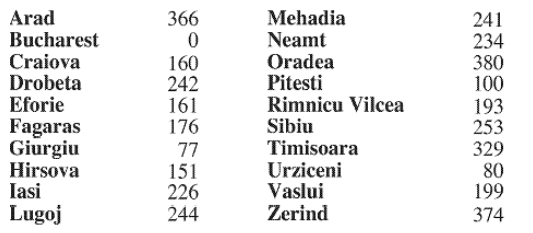
\includegraphics[width=0.75\textwidth]{images/esempio-euristica-h.png}
    \end{figure}
\end{example}

\subsection{Algoritmo di ricerca Best-first}
Il \textbf{best first - heuristic} usa lo stesso algoritmo di UC \footnote{Warning: AIMA ed. IV ha usato uno schema di
UC diverso e alcune proprietà cambiano} ma con uso di $f$ (stima di costo) per la coda con priorità.
Una volta scelta $f$ determina la strategia di ricerca. A ogni passo si sceglie il nodo sulla frontiera per cui il valore della $f$ è 
migliore (il nodo più promettente).
\begin{note}
    Migliore significa "minore" in caso di un'euristica che stima la distanza della soluzione
\end{note}
\hspace{-15pt}Un caso speciale: \textbf{greedy best-first}, su usa solo $h (f=h)$.
\begin{example}
    Esempio di greedy best-first con $f=h$
    \begin{figure}[h!]
        \centering
        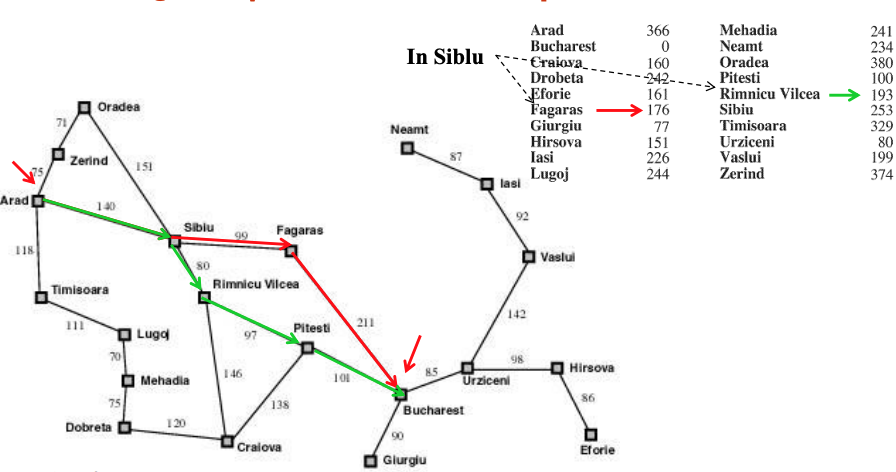
\includegraphics[width=0.75\textwidth]{images/esempio-best-first.png}
    \end{figure}
    Da Arad a Bucarest con \textbf{Greedy best-first}: Arad, sibiu, fagaras, bucharest (450) ma non è l'ottimale
    che sarebbe: Arad, Sibiu, Rimnicu, Pitesti, Bucarest (418).
\end{example}

\subsection{Algoritmo A}
Si può dire qualcosa di $f$ per avere garanzie di completezza e ottmialità?
\begin{definition}
    Un \textbf{Algoritmo A} è un algoritmo di best first con una fuzine di valutazione dello stato del tipo:
    $$f(n) = g(n) + h(n) \:\: \text{con}\:\: h(n) \geq 0 \:\: \text{e}\:\: h(goal) = 0$$
\end{definition}
In questa definizione abbiamo che $g(n)$ è il costo del cammino percorso per raggiugnere n, mentre $h(n)$ una
stima del costo per raggiungere da n un nodo goal (distanza).\\
Vedremo alcuni casi particolari dell'algoritmo A:
\begin{itemize}
    \item Se $h(n) = 0 \:\:[f(n) = g(n)]$ si ha \textbf{Ricerca Uniforme (UC)}.
    \item Se $g(n) = 0 \:\:[f(n) = h(n)]$ si ha \textbf{Greedy Best First}.
\end{itemize}
\begin{example}
    Esempio nel gioco dell'otto.
    \begin{figure}[h!]
        \centering
        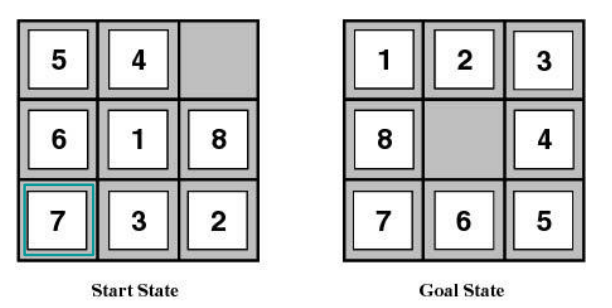
\includegraphics[width=0.6\textwidth]{images/esempio-gioco-otto.png}
    \end{figure}

    \hspace{-15pt}$f(n) = \#\text{mosse fatte} \:\: + \:\: \#\text{caselle-fuori-posto} \hspace{10pt} f(start) = 0 + 7 \hspace{10pt} f(goal-state) = ? + 0$\\
    Dopo $\leftarrow, \downarrow, \uparrow, \rightarrow$ abbiamo che $f = 4 + 7$, stesso stato, $g$ è cambiato.
\end{example}
\begin{theorem}
    L'algoritmo A con la condizione:
    $$g(n) \geq d(n) \cdot \epsilon \hspace{10pt}(\epsilon >0 \text{ costo minimo arco})$$
    è completo (con $d(n)$ che è la distanza).
\end{theorem}
\begin{note}
    La conzione ci garantisce che non si verifichino situazioni strane del tipo:
    \begin{figure}[h!]
        \centering
        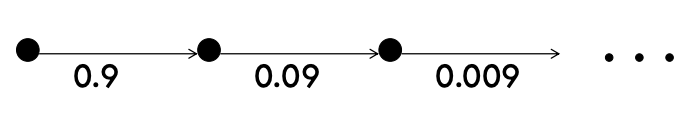
\includegraphics[width=0.65\textwidth]{images/nota-alg-completo.png}
    \end{figure}
    e quindi che il costo lungo un cammino non cresca "abbastanza" (se cresce abbastanza possiamo fermare quel path per costo alto di g).
\end{note}
\begin{demostration}
    Sia $[n_0, n_1, n_2, \dots, n', \dots, n_k = goal]$ un cammino soluzione. Sia $n'$ un nodo della frontiera su un cammino soluzione:
    $n'$ prima o poi sarà espanso. Infatti esistono solo un numero finito di nodi $x$ che possono essere aggiunti alla frontiera con $f(x) \leq f(n')$
    (è la condizione sulla crescita di g, scritta precedentemetne, tale che non esista una catena infinita di archi e nodi che possa aggiungere con costo sempre $\leq f(n')$).\\\\
    Quindi, se non si trova una soluzione prima, $n'$ verrà espanso e i suoi successori aggiunti alla frontiera. Tra questi anche il suo successore sul cammino soluzione.\\
    Il ragionamento si può ripetere fino a dimostrare che anche il nodo goal sarà selezionato per l'espanzione.
\end{demostration}

\subsection{Algoritmo $A^*$}
La funzione di valutazione ideale (oracolo):
$$f^*(n) = g^*(n) + h^*(n)$$
Con $g^*(n)$ il costo del cammino minimo da radice a n, $h^*(n)$ costo del cammino minimo da n a goal, $f^*(n)$ costo
del cammino minimo da radice a goal, attraverso n. Normalmente:
$$g(n) \geq g^*(n) \hspace{10pt} e \hspace{10pt} h(n) \text{ è una stima di } h^*(n)$$
($g(n) \geq g^*(n)$ rappresenta costo cammino $\geq$ costo migliore). Si può andare in sottostima (e.g. linea d'aria) o 
sovrastima della distanza dalla soluzione.
\begin{definition}[Euristica ammissibile]
    $$\forall n\:\: t.c.\:\: h(n) \leq h^*(n) \:\:\:\: \text{h è una sottostima}$$
\end{definition}
\begin{example}
    L'euristica della distanza in linea d'aria.
\end{example}
\begin{definition}[Algoritmo $A^*$]
    Un algoritmo A in cui h è una funzione euristica ammissibile.
\end{definition}
\begin{theorem}
    Gli algoritmi $A^*$ sono \textbf{ottimali}.
\end{theorem}
\begin{corollaries}
    $BF^{(+)}$ e UC sono ottimali ($h(n) = 0$).
\end{corollaries}
\begin{example}
    Itinerario con $A^*$ (ad albero).
    \begin{figure}[h!]
        \centering
        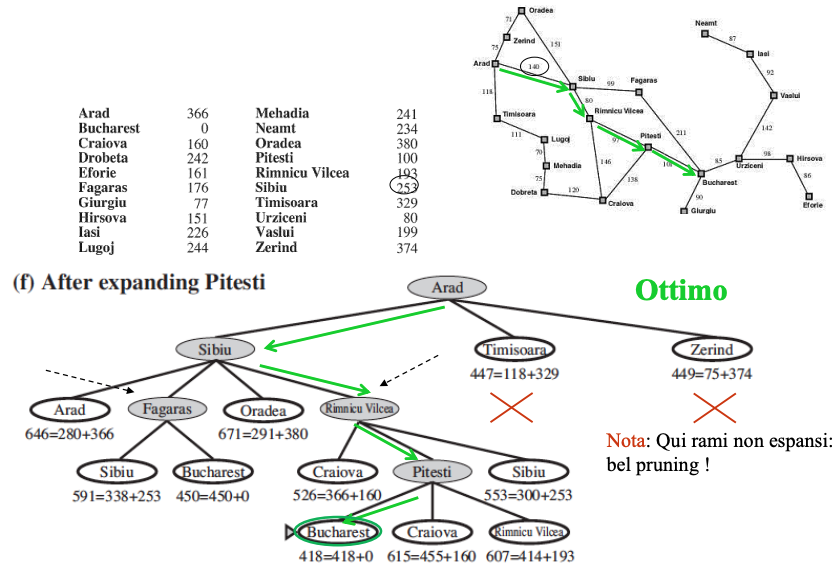
\includegraphics[width=0.62\textwidth]{images/itinerario-A*-albero.png}
    \end{figure}
\end{example}
\begin{observation}
    Alcune osservazioni su $A^*$
    \begin{enumerate}
        \item Rispetto a greedy best-first, la componente g fa si che si abbandonino cammini che vanno troppo in profondità.
        \item Ha sotto o sovra stima?
        \begin{enumerate}
            \item Una sottostima (h) può farci compiere del lavoro inutile (tenendo anche candidati non buoni), però non ci 
            fa perdere il cammino migliore (quando prendo nodo goal è il cammino migliore).
            \item Una funzione che qualche volta sovrastima può farci perdere la soluzione ottimale (taglio per causa di sovrastima, invece era buona)
        \end{enumerate}
    \end{enumerate}
\end{observation}

\subsubsection{Ottimalità su $A^*$}
\begin{wrapfigure}[8]{r}{5cm}
    \vspace{-30pt}
    \centering
    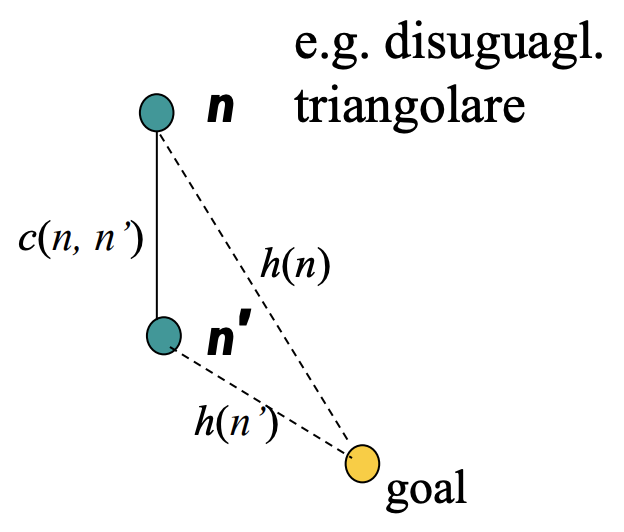
\includegraphics[width=4cm]{images/dis-triagolare.png}
\end{wrapfigure}
Nel caso di ricerca a/su albero l'uso di un'euristica ammissibile è sufficente a garantire l'ottimalità su $A^*$.
Nel caso di ricerca su grafo (con UC come visto) serve una proprietà più forte: la \textbf{consistenza} (detta anche \textbf{monotonicità}).\\\\
Per evitare rischio di scartare candidati ottimi (stato già incontrato) si vuol evitare, causa uso della lista esplorati, di far sparire, o meglio
non considerare al momento dell'espansione, candidati ottimali. Cerchiamo quindi condizioni per garantire che il primo espanso sia il migliore.

\begin{definition} 
    Un euristica \textbf{consistente} $[h(goal) = 0]$ (consistenza locale).
    $$\forall n \:\: t.c. \:\: h(n) \leq c(n, a, n') + h(n') \text{ dove n' è un successore di n}$$
\end{definition}
\hspace{-15pt}Ne segue che $f(n) \leq f(n')$
\begin{note}
    Se h è consistente la $f$ non decresce mai lungo i cammini, da cui il termine \textbf{monotona}.
\end{note}
\begin{theorem}
    Un'euristica monotona è ammissibile.
\end{theorem}
\hspace{-15pt}Esistono euristiche ammissibili che non sono monotone, ma sono rare. Le euristiche monotone garantiscino che la soluzione meno costosa 
venga trovata per rima e quindi sono ottimali anche nel caso di ricerca su grafo.\\
Non si devono recuperare tra gli antenati nodi con costo minore. Lista degli esplorati, stato già esplorato è sul cammino ottimo allora posso
evitare di inserire il corrente ripetuto senza perdere l'ottimalità.
\begin{lstlisting}
    if figlio.Stato non e in esplorati e non e in frontiera then
        frontiera = Inserisci(figlio, frontiera)
\end{lstlisting}
Per la frontiera, volendo evitare stati ripetuti, resta 'if' finale di UC:
\begin{lstlisting}
    if figlio.Stato e in frontiera con Costo-cammino piu alto then
        sostituisci quel nodo frontiera con figlio 
\end{lstlisting}
Andiamo ora a verificare l'ottimalità di $A^*$ supponendo di avere il teorema, con $h$ consistente.
\begin{enumerate}
    \item Se $h(n)$ è consistente i valori di $f(n)$ lungo un cammino sono non decrescenti:
    $$\text{se } h(n) \leq c(n, a, n') + h(n') \hspace{10pt} \Rightarrow \text{(def. consistenza sommando g(n))}\hspace{10pt} g(n) + h(n) \leq g(n) + c(n, a, n') + h(n')$$
    ma siccome abbiamo $g(n) + c(n, a, n') = g(n')$ allora
    $$g(n) + h(n) \leq g(n') + h(n') \Rightarrow f(n) \leq f(n') \Rightarrow f \text{ monotona}$$
    \item Ogni volta che $A^*$ seleziona un nodo (n) per l'espansione, il cammino ottimo a tale nodo è stato trovato: 
    se così non fosse, ci sarebbe un altro nodo m ella frontiera sul cammino ottimo (a n, ancora da trovare con un cammino ottimo), con $f(m)$
    minore (per la monotonia e n successore di m); ma ciò non è possibile perché tale nodo sarebbe già stato espanso (si espande prima un nodo con f minore).
    \item Quando seleziona nodo goal è cammino ottimo $[h=0, f=C^*]$.
\end{enumerate}
% TODO: AGGIUNGI IMMAGINI
Quindi, detto questo, perché $A^*$ è vantaggioso?
\begin{itemize}
    \item $A^*$ espande tutti i nodi con $f(n) < C^*$ ($C^*$ = costo ottimo)
    \item $A^*$ espande alcuni nodi con $f(n) = C^*$.
    \item \textbf{$A^*$ non espande alcun nodo con $f(n) > C^*$}
\end{itemize}
Quindi alcuni nodi (e suoi sottoalberi) non verranno considerati per l’ espansione (ma restiamo ottimali):
pruning (h opportuna, più alta possibile tra le ammissibili, fa tagliare molto).\\\\
% TODO: AGGIUNGI IMMAGINE
Più f è aderente a stima ottimale, più taglio! Ovali più stretti. Cercheremo quindi una h il più alta possibile tra le ammissibili
Se molto bassa molti (sino a tutti i) nodi restano minore di $C^* \to$ espando tutti (a cerchi).
Il pruning sotto-alberi è il punto focale: non li abbiamo già in memoria e evitiamo di generarli (decisivo per i problemi di AI a spazio stati esponenziali.\\\\
In riassunto L’algoritmo è quello degli schemi usati per UC, Usando f = g+h per la coda con priorità, ove h e g soddisfano quanto allo slide 9 [A], 
ove h è una funzione euristica ammissibile $[A^*]$, e considerando le condizioni dette per ottenere l’ottimalità su grafi.
\begin{itemize}
    \item $A^*$ è \textbf{completo}: discende dalla completezza di A ($A^*$ è un algoritmo A particolare).
    \item $A^*$ con euristica monotona è \textbf{ottimale}.
    \item $A^*$ è \textbf{ottimamente efficiente}: a parità di euristica nessn altro algoritmo espande meno nodi (senza rinunciare a ottimalità)
\end{itemize}
I problemi principali sono la scelta dell'euristica e  ancora l'occupazione di memoria che nel caso
pessimo resta esponenziale come visto per gli altri algoritmi di ricerca con stesso schema, causa frontiera.

\subsection{Sotto-casi speciali: US e Greedy Best First}
Ci sono due casi particolai dell'algoritmo A:
\begin{enumerate}
    \item Se $h(n) = 0$ $[f(n) = g(n)]$ si ha Uniform Cost (UC), ossia $g$ non basta (si può migliorare).
    \item Se $g(n) = 0$ $[f(n) = h(n)]$ si ha Greedy Best Fist, ossia $h$ non basta (già visto all'inizio).
\end{enumerate}
\subsubsection{UC vs $A^*$}
Illustrazione dell'algoritmo di ricerca Dijkstra per trovare il percorso da un nodo iniziale (in basso
sinistra, rosso) a un nodo obiettivo (in alto a destra, verde) in un problema di pianificazione del movimento del robot.
I nodi aperti rappresentano l'insieme "provvisorio". I nodi pieni sono quelli visitati, con colore
che rappresenta la distanza: più verde, più lontano. Nodi in tutti i diversi
le direzioni vengono esplorate in modo uniforme, apparendo come un fronte d'onda più o meno circolare
poiché l'algoritmo di Dijkstra utilizza un'\textbf{euristica identicamente uguale a 0}. $\to$ UC !\\\\
\begin{wrapfigure}[6]{r}{5cm}
    \vspace{-35pt}
    \centering
    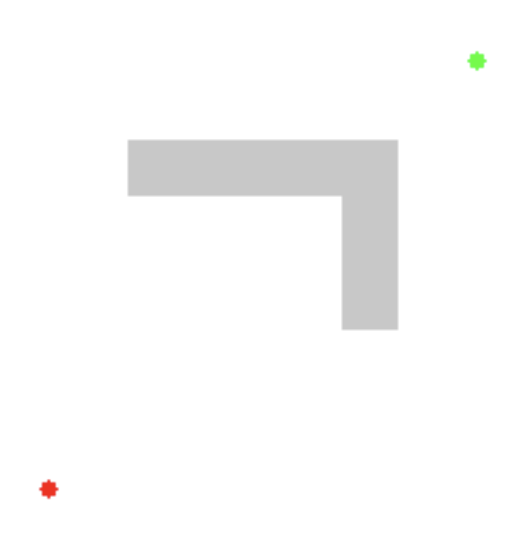
\includegraphics[width=3cm]{images/dijkstra.png}
\end{wrapfigure}
Illustrazione dell'algoritmo di ricerca A* per trovare il percorso da un nodo iniziale a un nodo obiettivo in un robot è un
problema di pianificazione del movimento. I cerchi vuoti rappresentano i nodi nell'insieme aperto, cioè,
quelli che restano da esplorare e quelli pieni sono nell'insieme chiuso. Colore acceso
ogni nodo chiuso indica la distanza dalla partenza: più è verde, più è lontano. Uno
può prima vedere A* muoversi in linea retta in direzione della porta, poi quando colpisce l'ostacolo, esplora percorsi alternativi attraverso i nodi da insieme aperto $\to$ frontiera.\\\\
L'algoritmo A* è una generalizzazione dell'algoritmo di Dijkstra che riduce le dimensioni del sottografo che deve essere esplorato, se il lower-bound
della "distanza" dall'obiettivo (h) è disponibile.

\subsection{Costruire le euristiche di $A^*$}
Partiamo dalle valutazione di funzioni euristiche. A parità di ammissibilità, una euristica può essere più
efficiente di un’altra nel trovare il cammino soluzione migliore (visitare meno nodi). Questo dipende da quanto
informata è l'euristia (dal \textbf{grado di informazione posseduto}) 
\begin{itemize}
    \item $h(n) = 0$ minimo di informazione (BF o UC)
    \item $h^*(n)$ massimo di infomrazione (oracolo)
\end{itemize}
In generale, per le euristiche ammissibili:
$$0 \leq h(n) \leq h^*(n)$$
\begin{theorem}
    Se $h_1 \leq h_2$, i nodi espansi\footnote{Ricorda che $A^*$ espande tutti i nodi con $f(n) = g(n) + h(n) < C^*$, e sono meno per $h$ maggiore (h maggiore fa andare più nodi oltre $C^*$).} da $A^*$ con $h_2$ sono un sottoinsieme di quelli espandi da $A^*$ con $h_1$.
\end{theorem}
\hspace{-15pt}Se $h_1 \leq h_2$, $A^*$ con $h_2$ è almeno efficiente quanto $A^*$ con $h_1$.
Un’euristica più informata (accurata) riduce lo spazio di ricerca (è più efficiente), ma è tipicamente più costosa da calcolare (e.g. un caso estremo ?)
\begin{example}
    Due euristiche ammissibili per il gioco dell'8 potrebbero essere le seguenti:
    \begin{itemize}
        \item $h_1$: conta il numero di caselle fuori posto
        \item $h_2$: somma delle distanze \textbf{Manhattan} (orizzonatle/verticale) delle caselle fuori posto dalla posizione finale.
    \end{itemize}
    $h_2$ è più informata di $h_1$, infatti $\forall n \:\:.\:\: h_1(n) \leq h_2(n)$, quindi si dice che $h_2$ \textbf{domina} $h_1$ (utile per confrontte tra ammissibili)
    \begin{figure}[h!]
        \centering
        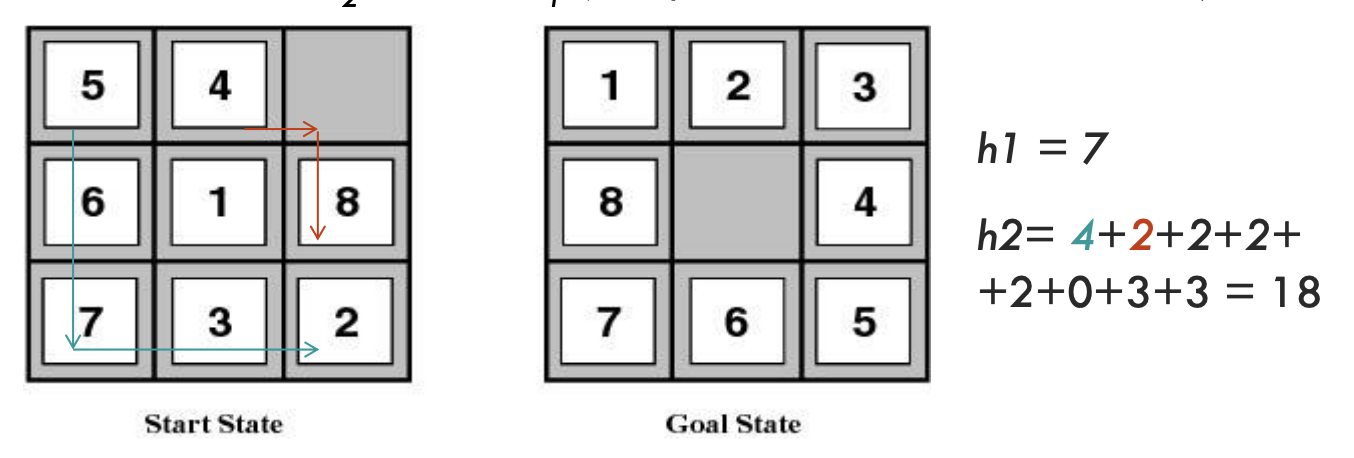
\includegraphics[width=0.65\textwidth]{images/euristica-gioco-8.png}
    \end{figure}
\end{example}
\begin{definition}
    La somma delle distanze Manghattan si definisce come:
    $$h((x,y)) = MD((x,y), (x_g, y_g)) = |x - x_g| + |y - y_g|$$
\end{definition}
\begin{figure}[h!]
    \centering
    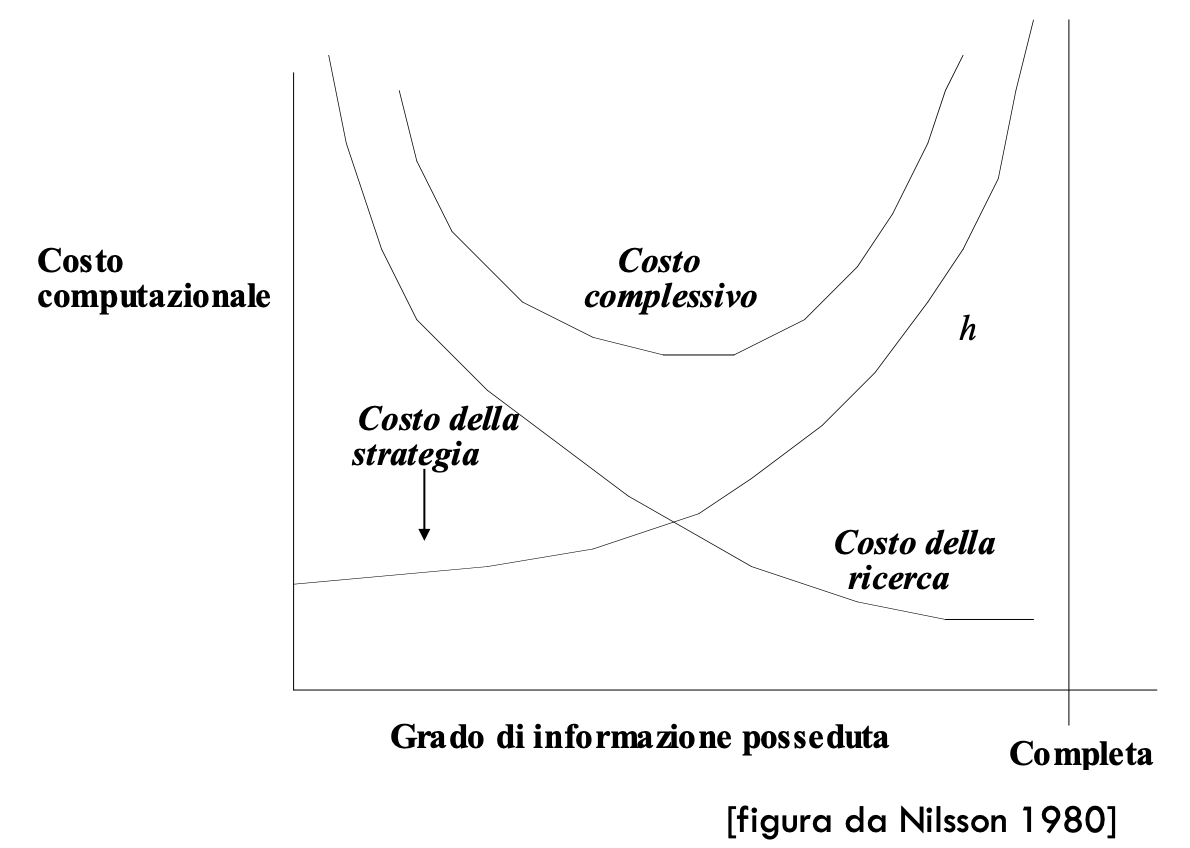
\includegraphics[width=0.60\textwidth]{images/costo-ricerva-vs-costo-euristica.png}
    \caption{Costo ricerca vs costo euristico}
\end{figure}
\hspace{-15pt}Ora capiamo come valutare gli algoritmi di ricerca euristica. Introfuciamo
il \textbf{fattore di diramazione effettivo} $b^*$, N: numero di nodi generati, d: profondità della soluzione.
$b^*$ è il fattore di diramazione di un albero uniforme con $N+1$ nodi, solizione dell'equazione:
$$N + 1 = b^* + (b^*)^2 + \dots + (b^*)^d$$
Sperimentalmente una buona euristica ha un $b^*$ abbastanza vicino a 1 (<1.5)
\begin{example}
    Ricodando l'esempio dal gioco dell'otto:
    \begin{figure}[h!]
        \centering
        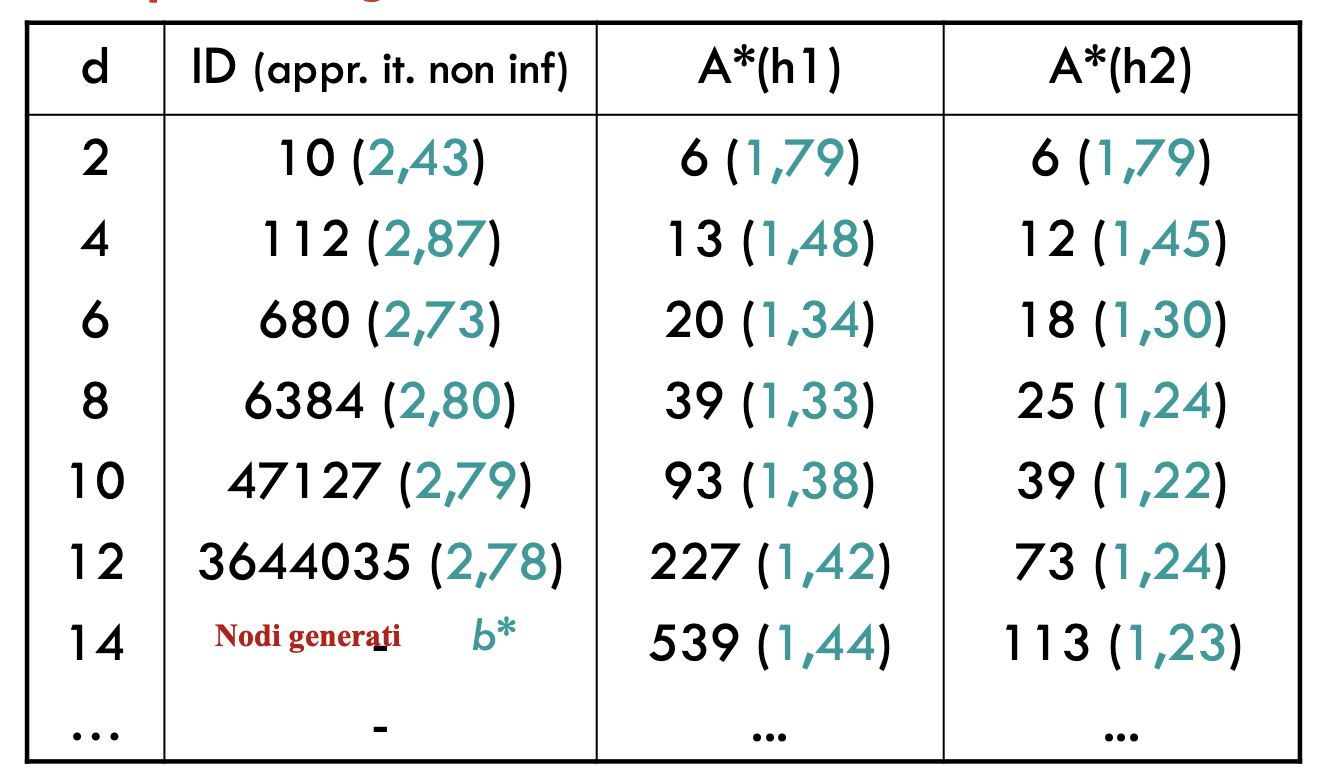
\includegraphics[width=0.60\textwidth]{images/gioco-otto-misura-euristiche.png}
    \end{figure}
    Sono riportati: Nodi generati e fattore di diramazione effettivo ($b^*$, verde)
    I dati sono mediati, per ogni d, su 100 istanze del problema [AIMA].\\\\
    Nella \textbf{capacità di esplorazione}, l'influenza di $b^*$:
    \begin{itemize}
        \item Con b=2: d=6 e N = 100 \hspace{15pt} d=12 e N = 10.0000
        \item Con b=1.5: d=12 N = 100 \hspace{15pt} d=24 e N = 10.000
    \end{itemize}
    migliorando di poco l’euristica si riesce, a parità di nodi espansi, a raggiungere una profondità doppia di esplorazione mosse!
\end{example}

\subsection{Inventare euristiche}
Quindi abbiamo che:
\begin{enumerate}
    \item Tutti i problemi dell’IA (o quasi) sono di complessità esponenziale ... (nel generare nodi, i.e. configurazioni possibili) ma c’è esponenziale e esponenziale!
    \item L’euristica può migliorare di molto la capacità di esplorazione dello spazio degli stati rispetto alla ricerca cieca.
    \item Migliorando anche di poco l’euristica si riesce ad esplorare uno spazio molto più grande (più in profondità).
\end{enumerate}
Per inventare un euristica ci sono alcune strategie, che aiutano appunto ad ottenre euristiche amissibili:
\begin{itemize}
    \item Rilassamento del problema
    \item Massimizzazione di euristiche
    \item Database di pattern disgiunti
    \item Combinazione lineare
    \item Apprendere dall’esperienza
\end{itemize} 
\subsubsection{Rillassamento problema}
\begin{example}
    Il rilassamento del problema nel gioco dell’8 mossa da A a B possibile se: 
    \begin{enumerate}
        \item \textbf{B adiacente a A}
        \item \textbf{B libera}
    \end{enumerate}
    $h_1$ e $h_2$ sono calcoli distanza esatta della soluzione in versioni semplificate del puzzle:
    \begin{itemize}
        \item $h_1$ (nessuna restrizione, ne 1 ne 2): sono sempre ammessi scambi a piacimento tra caselle (si muove
        ovunque) $\to$ numero caselle fuori posto.
        \item  $h_2$ (solo restrizione 1): sono ammessi spostamenti anche su caselle occupate, purché adiacenti $\to$ somma delle distanze Manhattan.
    \end{itemize}
\end{example}

\subsubsection{Massimizzazione di euristiche}
Se si hanno una serie di euristiche ammissibili $h_1, h_2, \dots, h_k$ \textbf{senza che nessuna "domini" un'altra}
allora conviene prendere il massimo dei lori valori:
$$h(n) = max(h_1(n), h_2(n), \dots, h_k(n))$$
Se le $h_i$ sono ammissibili, anche la $h$ lo è. La h domina tutte le altre.

\subsubsection{Database con pattern disgiunti}
\begin{figure}[h!]
    \centering
    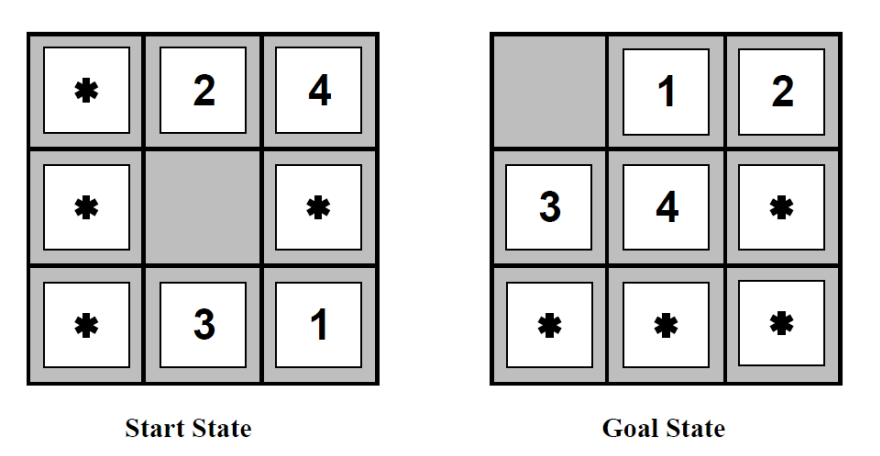
\includegraphics[width=0.65\textwidth]{images/euristiche-da-sottoproblemi.png}
\end{figure}
\hspace{-15pt}Costo della soluzione ottima al sottoproblema (di sistemare 1,2,3,4) è una sottostima del costo per il problema nel suo
complesso (e.g. rilevatesi più accurata della Manhattan). \\
\textbf{Database di pattern}: memorizzare ogni istanza del
sottoproblema con relativo costo della soluzione. Usare poi questo database per calcolare $h_{DB}$ (estraendo dal DB la
configurazione corrispondente allo stato completo corrente).
\begin{itemize}
    \item \textbf{Domanda}: Potremmo poi fare la stessa cosa per altri sottoproblemi: 5-6-7-8, 2-4-6-8, ottenendo altre euristiche ammissibili,
    poi prendere il valore massimo: ancora una euristica ammissibile. Ma potremmo sommarle e ottenere un’euristica
    ancora più accurata?
    \item \textbf{Risposta}: In generale no perché le soluzioni ai sottoproblemi interferiscono (condividono alcune mosse, se sposto 1-2-3-4, spostero
    anche 4-5-6-7) e la somma delle euristiche in generale non è ammissibile (potremmo sovrastimare avendo avuto aiuti mutui).
    Si deve eliminare il costo delle mosse che contribuiscono all’altro sottoproblema. Database di pattern disgiunti consentono di sommare i
    costi (euristiche additive) [e.g. solo costo mosse su1-2-3-4], sono molto efficaci: gioco del 15 in pochi ms
    ma per esempio difficile scomporre per cubo Rubik.
\end{itemize}

\subsubsection{Apprendimento dall'esperienza}
Bisogna eseguire un apprendimento dall'esperienza. Quindi far girare il programma, raccogliere dati: coppie
$<stato, h^*>$. Usare i dati per apprendere a predire la h con algoritmi di apprendimento induttivo (da istanze note stimiamo h in generale).\\
Gli algoritmi di apprendimento si concentrano su caratteristiche salienti dello stato (feature, xi) [e.g.
apprendiamo che da numero tasselli fuori posto 5 $\to$ costo~14, etc].

\subsubsection{Combinazione euristiche}
Quando diverse caratteristiche influenzano la bontà di uno stato, si può usare una combinazione lineare per combinare le euristiche:
$$h(n) = c_1 x_1(n) + c_2x_2(n) + \dots + c_k x_k(n)$$
\begin{example}
    Gioco dell'8: $h(n) = c_1 \:\: \#\text{fuori-posto} + c_2 \#\text{coppie-scambiate}$\\
    Scacchi: $h(n) = c_1 \:\text{vant-pezzi} + c_2 \:\text{pezzi-attacc.} + c_3 \:\text{regina} + \dots$
\end{example}
\hspace{-15pt}Il peso dei coefficienti può essere aggiustato con l’esperienza, anche qui apprendendo automaticamente da esempi di gioco.
$h(goal) = 0$ (e.g. gioco dell’8) ma ammissibilità e consistenza non automatiche.

\subsection{Algoritmi evoluti basati su $A^*$}
Ci sono una serie di algoritmi basati su $A^*$ che possono andare a portare ad un miglioramento dell'occupazione della memoria.
Fra questi abbiamo: Beam search, A* con approfondimento iterativo (IDA*), ricerca best-first ricorsiva (RBFS), A* con memoria limitata (MA*) in versione semplice (SMA*).

\subsubsection{Beam search}
Nel Best First viene tenuta tutta la frontiera; se l’occupazione di memoria è eccessiva si può ricorrere ad una variante: la Beam search.
La Beam Search tiene ad ogni passo solo i k nodi più promettenti, dove k è detto l’ampiezza del raggio
(beam). La Beam Search non è completa.

\subsubsection{IDA${}^*$}
L'$IDA^*$ è un $A^*$ con approfondimento iterativo. IDA* combina A* con ID: ad ogni iterazione si ricerca
in profondità con un limite (cut-off) dato dal valore della funzione f (e non dalla profondità) il limite f-limit viene aumentato ad ogni iterazione,
fino a trovare la soluzione. Punto critico: di quanto viene aumentato f-limit.
\begin{example}
    \begin{figure}[h!]
        \centering
        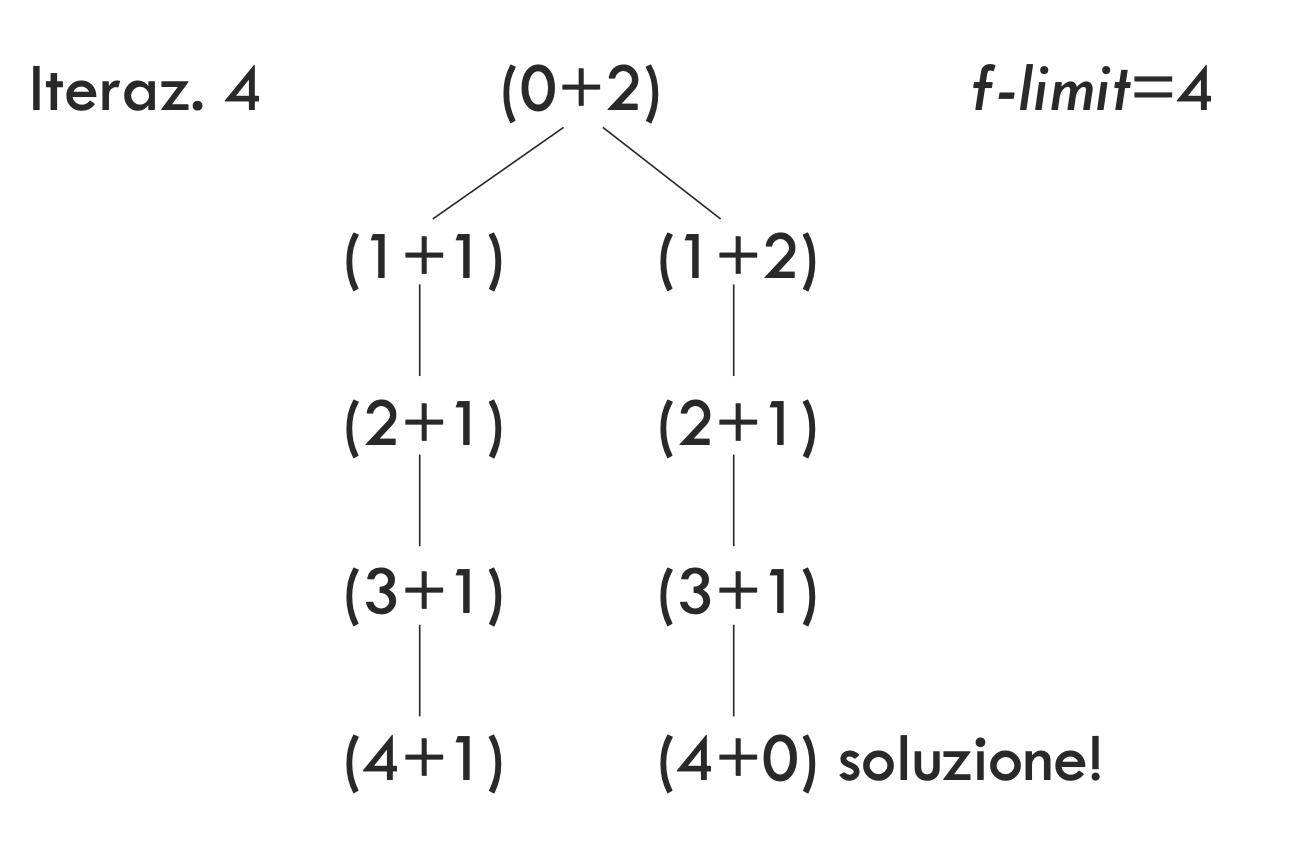
\includegraphics[width=0.65\textwidth]{images/esempio-ida*.png}
    \end{figure}
\end{example}
\hspace{-15pt}Cruciale la scelta dell'incremento per garantire l’ottimalità:
\begin{itemize}
    \item Nel caso di costo delle azioni fisso è chiaro: il limite viene incrementato del costo delle azioni.
    \item Nel caso che i costi delle azioni siano variabili? O costo minimo, oppure si potrebbe ad ogni passo fissare il limite successivo al
    valore minimo delle f scartate (in quanto superavano il limite) all’iterazione precedente.
\end{itemize}
$IDA^*$ è sia completo che ottimale.
\begin{itemize}
    \item Se le azioni hanno costo costante k (caso tipico 1) e f-limit viene incrementato di k.
    \item Se le azioni hanno costo variabile e l'incremento di f-limit è $\leq \epsilon$ (minimo costo degli archi).
    \item Se il nuovo f-limit = min. valore f dei nodi generati ed esclusi all'iterazione precedente.
\end{itemize}
L'occupazione di memoria è $O(bd)$.

\subsubsection{Best-first ricorsivo (BRFS)}
Simile a DF ricorsivo: cerca di usare meno memoria, facendo del lavoro in più. Tiene traccia ad ogni livello del \textbf{migliore percorso
alternativo}. Invece di fare backtracking in caso di fallimento (DF si ferma solo in fondo) interrompe l’esplorazione quando
trova un nodo meno promettente (secondo f). Nel tornare indietro si ricorda il miglior nodo che ha
trovato nel sottoalbero esplorato, per poterci eventualmente tornare Memoria: lineare nella profondita delle sol. ottima.
\begin{example}
    \begin{figure}[h!]
        \centering
        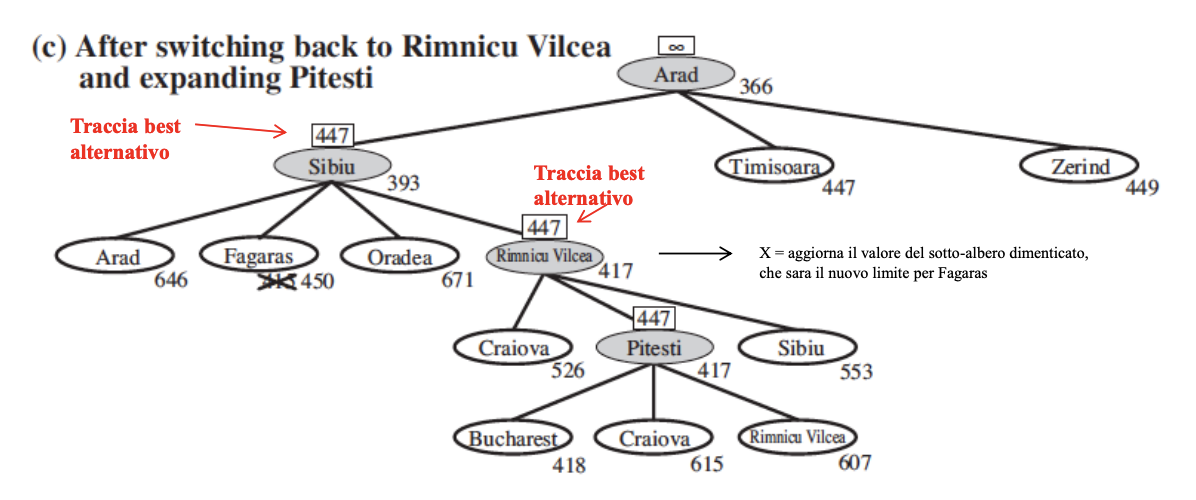
\includegraphics[width=0.65\textwidth]{images/esempio-best-first-ricorsivo.png}
    \end{figure}
\end{example}
\begin{lstlisting}
    function Ricerca-Best-First-Ricorsiva(problema)
        returns soluzione oppure fallimento
        // all inizio f-limite e un valore molto grande
        return RBFS(problema, CreaNodo(problema.Stato-iniziale), infinito) 

    function RBFS (problema, nodo, f-limite)
        // restituisce due valori
        returns soluzione oppure fallimento e un nuovo limite all f-costo 
        if problema.TestObiettivo(nodo.Stato) then return Soluzione(nodo)
        successori = [ ]

        for each azione in problema.Azioni(nodo.Stato) do
            aggiungi Nodo-Figlio(problema, nodo, azione) a successori // genera i successori
        if successori vuoto then return fallimento, infinito

        for each s in successori do // valuta i successori
            s.f = max(s.g + s.h, nodo.f) // un modo per rendere monotona f
        loop do
            migliore = il nodo con f minimo tra i successori
            if migliore.f > f_limite then return fallimento, migliore.f
            alternativa = il secondo nodo con f minimo tra i successori
            risultato, migliore.f = RBFS(problema, migliore, min(f_limite, alternativa))
            if risultato != fallimento then return risultato
\end{lstlisting}

\subsubsection{$A^*$ con memoria limitata (versione semplice)}
L'idea è quella di utilizzare al meglio la memoria disponibile. $SMA^*$ procede come $A^*$ fino ad esaurimento della
memoria disponibile. A questo punto \textbf{“dimentica” il nodo peggiore}, dopo avere aggiornato il valore del padre.
A parità di f si sceglie il nodo migliore più recente e si dimentica il nodo peggiore più vecchio. Ottimale se il cammino soluzione sta in memoria.\\\\
In conclusione in algoritmi a memoria limitata (IDA* e SMA*) le limitazioni della memoria possono portare a compiere
molto lavoro inutile [esp. ripetuta stessi nodi]. Difficile stimare la complessità temporale effettiva. Le limitazioni di memoria possono rendere un problema intrattabile dal punto di vista computazionale.
	% !TeX spellcheck = it_IT
\newpage
\section{Ricerca locale}
La ricerca \emph{euristica} nello spazio di stati è troppo costosa ed è quindi necessario utilizzare metodi diversi. \\ Se prima gli algoritmi restituivano un cammino soluzione per raggiungere un goal, ora il goal è la soluzione stessa al problema. Gli algoritmi di ricerca locale sono adatti per problemi in cui:
\begin{itemize}
	\item La sequenza di azioni non è importante ma conta solo lo stato goal
	\item Tutti gli elementi della soluzioni sono nello stato ma alcuni vincoli sono violati
\end{itemize}
Questi algoritmi non sono sistematici e tengono traccia solo del nodo corrente spostandosi su quelli adiacenti. \\
Non tengono traccia dei cammini: rendono più efficiente l'occupazione della memoria e possono trovare soluzioni anche in spazi di stati molto grandi o infiniti.\\
Sono utili per risolvere problemi di \textbf{ottimizzazione}:
\begin{itemize}
	\item Stato migliore secondo una funzione obiettivo $f$
	\item Lo stato di costo minore (non il cammino)
\end{itemize}
Data la funzione euristica del costo dell'obiettivo
\begin{center}
	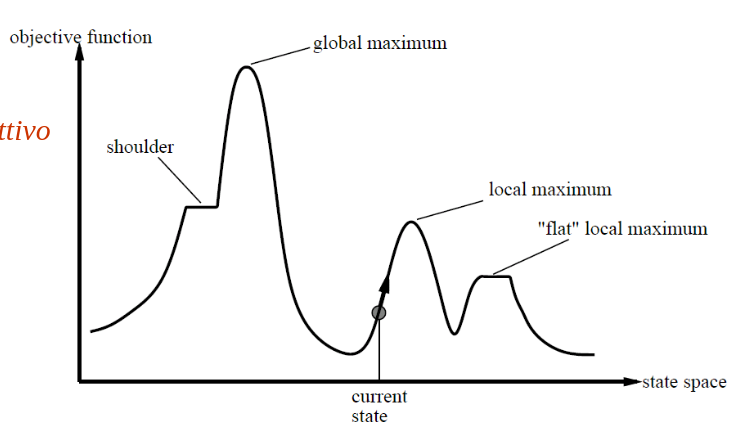
\includegraphics[scale=0.4]{ricerca_locale_spazio_stati.png}
\end{center}
uno stato ha una posizione sulla superficie e un'altezza che corrisponde al valore della valutazione della funzione obiettivo. Un algoritmo provoca movimento sulla superficie e l'obiettivo è raggiungere un punto in particolare (e.g. massimo locale).
\subsection{Hill climbing}
Sfrutta un principio di ricerca locale greedy dove vengono generati i successori e vengono valutati. Viene scelto un nodo che migliora lo stato attuale e scartati gli altri:
\begin{itemize}
	\item \textbf{Salita rapida} (o discesa): viene scelto il migliore
	\item \textbf{Stocastico}: scelta random
	\item \textbf{Prima scelta}: viene scelto il primo 
\end{itemize}
Se non ci sono successori che migliorano lo stato, l'algoritmo termina con fallimento.
\begin{lstlisting}[language=Python]
	def hill_climbing(problem):
		current = Node(problem.initial_state)
		while True:
			neighbors = [current.child_node(problem, action) for action in problem.actions(current.state)]
			if not neighbors: # se current non ha successori esci e restituisci current
				break
			# scegli il vicino con valore piu' alto (sulla funzione problem.value)
			neighbor = (sorted(neighbors,key = lambda x:problem.value(x), reverse = True))[0]
			if problem.value(neighbor) <= problem.value(current):
				break
			else:
				current = neighbor # (altrimenti, se vicino migliore, continua)
		return current
\end{lstlisting}
Non c'è frontiera a cui ritornare e si tiene un solo stato, quindi efficiente per la memoria. Il tempo necessario è variabile e dipende dal punto di partenza.\\

\subsubsection{8 regine}
Nel problema già descritto delle 8 regine, poniamo come funzione da minimizzare $h$ il numero di coppie di regine che si attaccano a vicenda. Bisogna minimizzare $h$.
Ogni regina può fare 7 mosse quindi abbiamo $7\cdot 8 = 56$ possibili stati successivi. Tra i migliori con lo stesso valore di $h$ si sceglie a caso.
\begin{example}[8 regine]
	Nel caso delle 8 regine:
	\begin{center}
		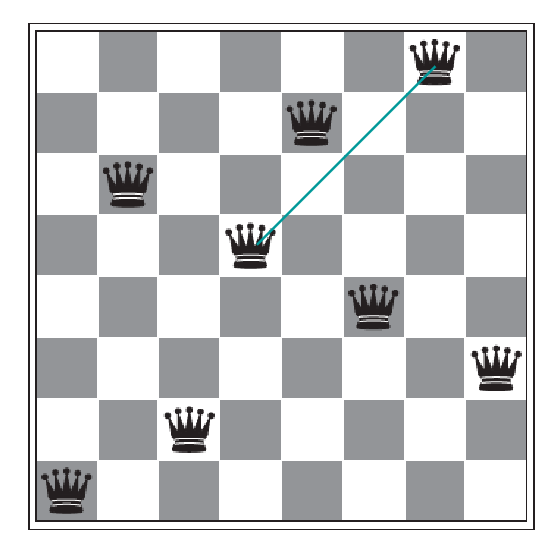
\includegraphics[scale=0.2]{8_regine_hill_climbing.png}
	\end{center}
\end{example}
Possiamo migliorare l'algoritmo in alcuni modi:
\begin{enumerate}
	\item Consentire un numero limitato di \textbf{mosse laterali}, ovvero l'algoritmo si ferma solo quando è peggiore la soluzione e non peggiore o uguale (sulle 8 regine $94\%$ di successo ma in media 21 passi)
	\item Hill-climbing \textbf{stocastico} (più lento ma soluzioni migliori)
	\item Hill-climbing \textbf{prima scelta}: genera mosse a caso fino a trovarne una migliore.
	\item Implementiamo un \textbf{riavvio casuale} che fa ripartire l'algoritmo da un punto a caso. Se la probabilità di successo è $p$, saranno necessarie $\frac{1}{p}$ iterazioni. Con molti minimi locali nella funzione obiettivo, $p$ si abbassa e aumentano il numero di volte in cui si blocca.
\end{enumerate}

\subsection{Tempra simulata}
Questo algoritmo combina hill-climbing con una scelta stocastica non totalmente casuale.\\
Ad ogni passo si sceglie un successore $n'$ a caso:
\begin{itemize}
	\item Se \textbf{migliora} lo stato corrente, viene espanso
	\item Se lo \textbf{peggiora} ($\Delta E = f(n')-f(n) \leq 0$) quel nodo viene scelto con probabilità $p=e^{\frac{\Delta E}{T}} \quad 0 \leq p \leq 1$.
\end{itemize}
Questo significa che $p$ è inversamente proporzionale al peggioramento. Con il progredire dell'algoritmo rende improbabili le mosse peggiorative.
\subsubsection{Scelta dei parametri}
I parametri sono il valore iniziale e il decremento di $T$. Il valore iniziale dovrebbe essere tale che per i valori medi di $\Delta E$ $p$ sia circa $0.5$.

\subsection{Local beam}
Dato l'algoritmo \emph{beam}, vengono salvati in memoria solo $k$ stati. Ad ogni passo si generano i successori di tutti i $k$ stati e:
\begin{itemize}
	\item Se si trova un goal, ci si ferma
	\item Altrimenti si prosegue con i $k$ migliori tra questi
\end{itemize}
\begin{note}
	È diverso da $k$ restart, in quanto non si riparte da $0$, e dal \emph{beam search} perché non si tengono tutti gli stati.
\end{note}
\subsubsection{Versione stocastica}
Si introduce un elemento di casualità: i $k$ successori vengono scelti con una probabilità maggiore per i migliori ma non tutti.
Introduciamo della terminologia:
\begin{itemize}
	\item \textbf{Organismo}: lo stato
	\item \textbf{Progenie}: i successori
	\item \textbf{Fitness}: il valore della funzione obiettivo
\end{itemize}

\subsubsection{Algoritmi genetici ed evolutivi}
Sono una variante della \emph{beam search stocastica} in cui gli stati successori sono ottenuti combinando due stati genitore invece che per evoluzione.
La \textbf{popolazione} iniziale è composta da $k$ \textbf{individui} generati casualmente e rappresentati come una stringa.
Gli individui sono valutati da una funzione di \textbf{fitness}. Vengono poi selezionati quelli per l'\textbf{accoppiamento} che danno vita alla generazione successiva in due modi:
\begin{itemize}
	\item \textbf{Crossover}: combinando il materiale genetico
	\item \textbf{Casuale}: con un meccanismo di mutazione genetica
\end{itemize}
Ogni generazione dovrebbe essere migliore della precedente.
\begin{example}[8 regine]
	Nel problema delle 8 regine abbiamo una popolazione di queste, dove le loro posizioni sono descritte da una stringa (ogni cifra è la riga in cui c'è la regina in quella colonna). La funzione di fitness è il numero di coppie di regine che non si attaccano.
	Per ogni coppia di combinazioni sulla scacchiera (scelta con la probabilità proporzionale alla fitness) viene scelto un punto di \textbf{crossing over} in maniera casuale e vengono generati due figli scambiandosi dei pezzi. Alla fine viene fatta una mutazione causale.
	\begin{center}
		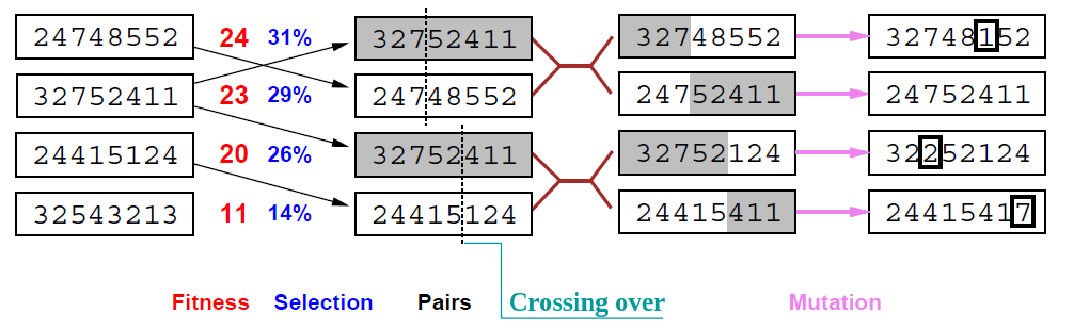
\includegraphics[scale=0.3]{alg_gen_ex.png}
	\end{center}
	\begin{center}
		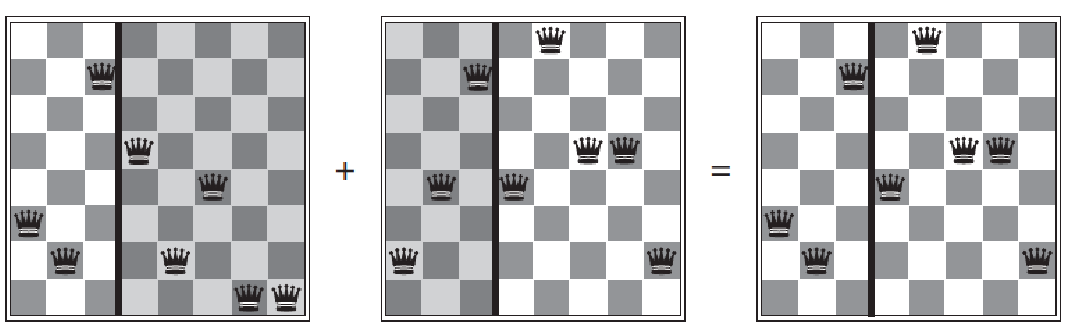
\includegraphics[scale=0.3]{alg_gen_ex_2.png}
	\end{center}
\end{example}
\noindent Questi algoritmi fanno parte del \textbf{Natural computer} e come vantaggi hanno:
\begin{itemize}
	\item Tendenza a salire della beam search stocastica
	\item Interscambio delle informazioni tra thread paralleli di ricerca in maniera indiretta
\end{itemize}
Questo tipo di algoritmi sono più efficaci se il problema ha componenti significative rappresentate in stringhe; è proprio la rappresentazione ad essere il punto critico.

\subsection{Spazi continui}
Lo stato è descritto da variabili \textbf{continue} in un vettore $x = x_1, \ldots, x_n$. Un esempio è lo spazio tridimensionale.\\
L'apparente difficoltà dovuta ai fattori di ramificazione infiniti è affrontata tramite strumenti matematici quali il \emph{gradiente}. Ad esempio l'\textbf{hill climbing iterativo} diventa:
\begin{equation*}
	x_{new} = x \pm \eta \nabla f(x)
\end{equation*}
sfruttando la direzione e lo spostamento che ci fornisce il gradiente invece di cercarlo tra gli infiniti successori.

\begin{example}
	Prendiamo la funzione $f(x)=x^2$ con derivata prima $f'(x)=2x$. Cerchiamo il minimo con
	\begin{equation*}
		x_{new}=x-\eta f'(x)
	\end{equation*}
	Partendo ad esempio da $x=2$ con $\eta=0.2$, otteniamo come primo risultato $x_{new} = 2-0.8=1.2$.
\end{example}

\subsection{Ambienti realistici}
A differenza dei problemi classici, il nostro ambiente è \textbf{parzialmente osservabile} e \textbf{non deterministico}. Qui le \textbf{percezioni} sono importanti in quanto restringono gli stati possibili e informano sull'effetto dell'azione.\\
L'agente deve elaborare una strategia con un piano di contingenza che tenga conto delle diverse eventualità.
\begin{example}[Aspirapolvere]
	\label{example:aspirapolvere}
	Un aspirapolvere imprevedibile ha due comportamenti:
	\begin{itemize}
		\item Se aspira in una stanza sporca la pulisce ma a volte pulisce anche una stanza adiacente
		\item Se aspira in una stanza pulita, a volte la sporca
	\end{itemize}
	La soluzione non è più una sequenza ma è un albero che gestisce il piano di di contingenza.
\end{example}

\subsubsection{Albero AND-OR}
È un albero che ha come nodi \emph{OR} le scelte dell'agente e come nodi \emph{AND} le diverse contingenze da considerare.
\begin{example}[Aspirapolvere]
	Nell'esempio \ref{example:aspirapolvere} l'albero sarebbe:
	\begin{center}
		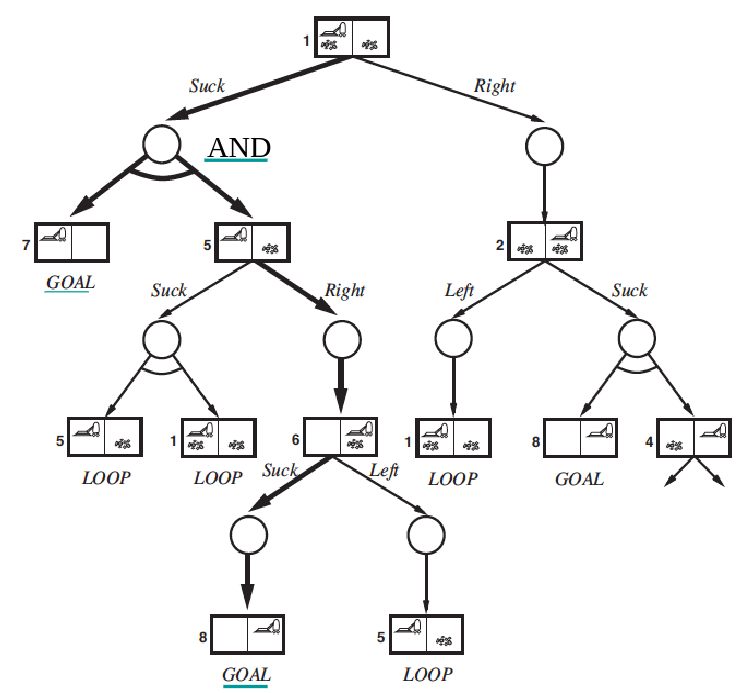
\includegraphics[scale=0.2]{example_aspirapolvere.png}
	\end{center}
\end{example}
	% !TeX spellcheck = it_IT
\newpage
\section{Agenti basati su conoscenza}
C'è bisogno di rappresentare la conoscenza in maniera parziale e incompleta (gli ambienti sono parzialmente osservabili). Ci servono quindi dei linguaggi più espressivi e con \textbf{capacità inferenziali}.\\
\subsection{Knowledge Base}
L'insieme di tutta la conoscenza necessaria a decidere un'azione da compiore è la \textbf{knowledge base} e può essere definita in due modi:
\begin{itemize}
	\item \textit{Dichiarativo}: all'agente viene detto cosa deve sapere, partendo da una conoscenza di base vuota e aggiungendo progressivamente formule (TELL)
	\item \textit{Procedurale}: si scrive un programma che definisca il processo decisionale una volta per tutte
\end{itemize}

\begin{definition}[Knowledge Base]
	Un insieme di \emph{enunciati} (formule) espressi in un linguaggio di rappresentazione.
\end{definition}

\begin{example}[Wumpus World]
	\label{example:wumpus_world}
	Il mondo del Wumpus è una caverna fatta di stanze connesse tra loro. All'interno c'è questa bestia puzzolente che mangia chiunque entri nella stanza in cui si trova. Questo può essere ucciso dall'agente che ha una freccia a disposizione.\\
	Ci sono delle stanze con degli \textit{ostacoli}: pozzi, in cui se l'agente entra, muore. In una delle stanze si trova l'\textit{obiettivo}, ovvero un lingotto d'oro.\\
	L'agente non conosce l'ambiente e la sua posizione, se non all'inizio.
	\begin{center}
		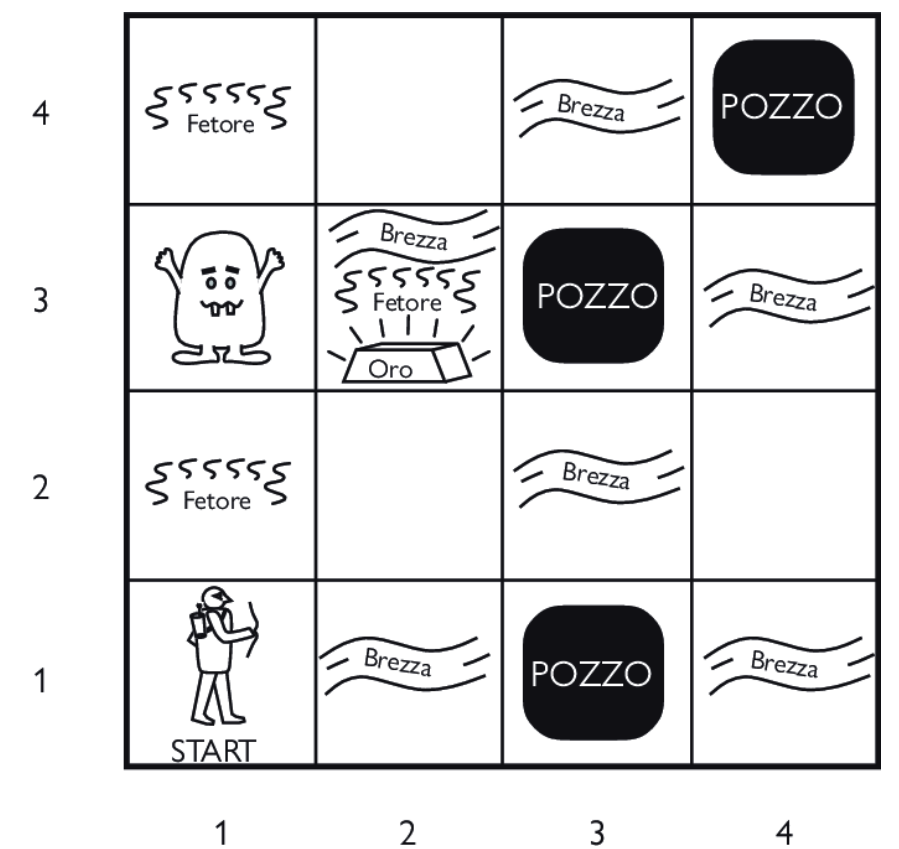
\includegraphics[scale=0.21]{wumpus_world.png}
	\end{center}
	Definiamo le \textbf{misure di prestazione}:
	\begin{itemize}
		\item +1000 se trova l'oro, torna in [1,1] ed esce
		\item -1000 se muore
		\item -1 per ogni azione
		\item -10 se usa la freccia
	\end{itemize}
	Invece l'\textbf{ambiente} è una griglia 4x4 circondata da pareti di delimitazione. L'agente inizia sempre nella posizione [1,1] rivolto verso destra (la prima casella è sempre safe). Le posizioni dell'oro e della bestia sono casuali e tutti i riquadri hanno una probabilità di $0.2$ di contenere un pozzo.\\
	L'agente può fare le seguenti \textbf{azioni}:
	\begin{itemize}
		\item Andare avanti
		\item Ruotare a destra o a sinistra di $90°$
		\item Afferrare un oggetto
		\item Scagliare la freccia
		\item Uscire
	\end{itemize}
	Il nostro agente puo \textbf{percepire} le seguenti cose:
	\begin{itemize}
		\item \textit{Fetore} nelle caselle adiacenti alla bestia
		\item \textit{Brezza} nelle caselle adiacenti ai pozzi
		\item \textit{Luccichio} nella casella con l'oro
		\item \textit{Urlo} se la bestia viene uccisa
	\end{itemize}
	e vengono rappresentati come una quintupla, che ad  esempio nella prima casella vale:
	\begin{equation*}
		[none,none,none,none,none]
	\end{equation*}
	Di conseguenza sappiamo che nelle caselle adiacenti non ci sono né pozzi né la bestia.
\end{example}

\subsubsection{Tell-Ask}
L'agente interagisce con la knowledge base tramite un'interfaccia funzionale di tipo Tell-Ask:
\begin{itemize}
	\item \textit{Tell}: aggiungere nuovi enunciati
	\item \textit{Ask}: interagire con la knowledge base
	\item \textit{Retract}: eliminirare enunciati
\end{itemize}
Gli enunciati nella KB rappresentano le credenze dell'agente e le risposte $\alpha$ devpomp essere tali per cui queste discendano necessariamente dalla KB.\\
Il problema fondamentale è quindi capire, data una base di conoscenza KB, come dedurre che un certo fatto $\alpha$ è vero di conseguenza.
\begin{equation}
	KB \models \alpha
\end{equation}
Un programma basilare è il seguente:
\begin{lstlisting}
	function Agente-KB (percezione) returns azione
		persistent: KB, una base di conoscenza
			t, un contatore, inizialmente a 0, che indica il tempo
		TELL(KB, Costruisci-Formula-Percezione(percezione, t ))
		azione = ASK(KB, Costruisci-Query-Azione( t ))
		TELL(KB, Costruisci-Formula-Azione(azione, t ))
		t = t + 1
		return azione
\end{lstlisting}
\subsubsection{Analisi}
A differenza di una \textit{base di dati}, la base di conoscenza non contiene solo fatti specifici da recuperare ma anche fatti generali, oregole, espressi in maniera esplicita in un linguaggio compatto. Questo le conferisce la \textbf{capacità inferenziale}, ovvero derivare nuovi fatti da quelli memorizzati.\\
Il lato negativo è che, avendo un linguaggi  più espressivo, è \textbf{meno efficiente} il meccanismo inferenziale. Serve quindi trovare il giusto bilanciamento da \textit{espressività} del linguaggio e \textit{complessità} del meccanismo inferenziale.

\subsection{Logica}
Le KB sono costituite da enunciati espresse secondo le regole della \textbf{sintassi}. La \textbf{semantica} invece ne esprime il significato. Un \textbf{modello} è una configurazione dei valori di verità che si possono assegnare alle variabili di una formula.
\subsubsection{Formalismo}
Un formalismo per la rappresentazione della conoscenza si compone di:
\begin{itemize}
	\item Una \textbf{sintassi}: un linguaggio composto da un vocabolario e da regole per la formulazione degli enunciati
	\item Una \textbf{semantica}: stabilisce una corrispondenza tra gli enunciati e ifatti del mondo
	\item Un \textbf{meccanismo inferenziale} che ci consente di inferire nuovi fatti
\end{itemize}
\begin{center}
	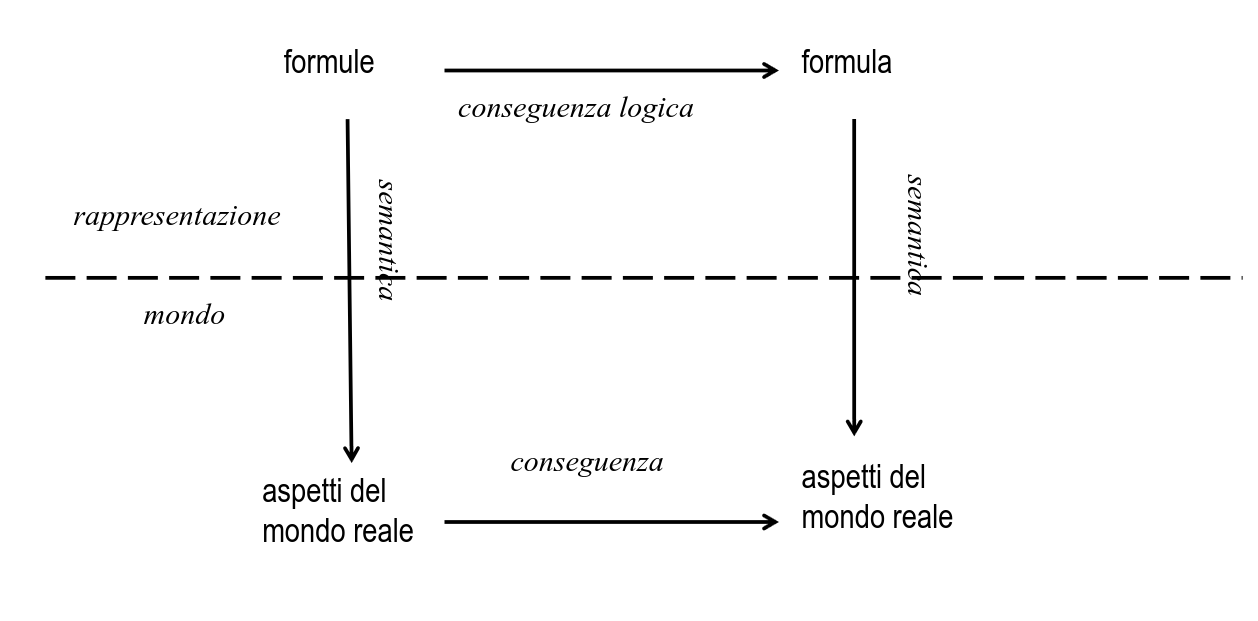
\includegraphics[scale=0.25]{formalismo.png}
\end{center}
Facendo il paragone con l'agente, le formule sono le sue configuraziini fisiche e il ragionamento è il processo di costruzione di nuove configurazioni a partire dalle vecchie. Il ragionamento logico deve assicurare che le nuove configurazioni siano effettive conseguenze sul mondo causate dalle vecchie configurazioni.

\section{Logica proposizionale}
\subsection{Sintassi}
La sintassi è la seguente, rappresentata in BNF:
\begin{equation}
	\begin{split}
		formula & \to formulaAtomica \vert formulaComplessa \\
		formulaAtomica & \to True \vert False \vert simbolo \\
		simbolo & \to P \vert Q \vert R \vert \ldots \\
		formulaComplessa & \to \neg formula \\
		&\vert (formula \land formula) \\
		& \vert (formula \lor formula)\\
		& \vert (formula \Rightarrow formula)\\
		& \vert (formula \Leftrightarrow formula)
	\end{split}
\end{equation}

\subsection{Semantica}
La logica proposizionale segue una semantica \textbf{composizionale}, dove il significato di una frase è determinato dal significato dei suoi componenti a partire dai \textit{simboli proposizionali}. Di seguito la ravola di verità:
\begin{table}[h!]
	\centering
	\begin{tabular}{|cc|ccccc|}
		\hline
		$P$ & $Q$ & $\neg P$ & $P \land Q$ & $P \lor Q$ & $ P \Rightarrow Q$ & $P \Leftrightarrow Q$\\
		\hline
		false & false & true & false & false & true & true \\
		false & true & true & false & true & true & false \\
		true & false & false & false & true & false & false \\
		true & true & false & true & true & true & true\\
		\hline
	\end{tabular}
\end{table}

\subsection{Conseguenza logica}
\begin{definition}[Conseguenza logica]
	Una formula $\alpha$ è una conseguenza logica di un insieme di formule KB se e solo se in ogni modello di KB, anche $\alpha$ è vera ($KB \models \alpha$).
\end{definition}
Indichiamo con $M(KB)$ i modelli dell'insieme di formule in KB e con $M(\alpha)$ l'insieme delle interpretazioni che rendono $\alpha$ vera, ovvero i suoi \textbf{modelli}.
\begin{equation}
	KB \models \alpha \Leftrightarrow M(KB) \subseteq M(\alpha)
\end{equation}

\subsubsection{Model checking}
Un modo per determinare la conseguenza logica è quello di enumere i \textit{modelli} e mostrare che la formula $\alpha$ vale in tutti quelli in cui è vera la KB.

\begin{example}[Wumpus World]
	\label{example:wumpus_world_model_checking}
	Partendo dall'esempio \ref{example:wumpus_world} abbiamo che la KB iniziale, $KB_0$, è costituita dalle regole descritte nella definizione dell'esercizio:
		\begin{gather*}
			\neg W_{1,1} \quad \neg P_{1,1} \\
			B_{2,1} \Leftrightarrow (P_{1,1} \lor P_{2,2,} \lor P_{3,1})\\
			B_{1,1} \Leftrightarrow (P_{1,2} \lor P_{2,1})\\
			\vdots
		\end{gather*}
		Il primo passo dell'agente è spostarsi in $[2,1]$ dato che in $[1,1]$ non ha percepito niente. Abbiamno quindi:
		\begin{equation*}
			KB_1 = KB_0 \cup \{\neg B_{1,1}, B_{2,1}, \neg F_{1,1}, \neg F_{2,1}, \ldots\}
		\end{equation*}
		e rappresentiamo le domande sulla presenza o meno di pozzi come:
		\begin{equation*}
			\begin{split}
				KB_1 \models \neg P_{1,2} \\
				KB_1 \models \neg P_{2,2} \\
				KB_1 \models \neg P_{3,1} \\
			\end{split}
		\end{equation*}
		Sapendo da $KB_0$ che non ci sono pozzi nella casella $[1,1]$ e che c'è un pozzo nella stanza adiacente solo se ci percepisce la brezza, formuliamo le seguenti proposizioni:
		\begin{equation*}
			\begin{split}
				& B_{1,1} \Leftrightarrow (P_{1,2} \lor P_{2,1}) \\
				& B_{2,1} \Leftrightarrow (P_{1,1} \lor P_{2,2} \lor P_{3,1})
			\end{split}
		\end{equation*}
		e concludiamo che non c'è brezza in $[1,1]$ e c'è in $[2,1]$, ovvero $\neg B_{1,1}$ e $B_{2,1}$.\\
		Ci rimangono quindi tre configurazioni possibili dato che abbiamo:
		\begin{gather*}
			KB_1 \models \neg P_{1,2}\\
			KB_1 \models P_{2,2}\lor P_{3,1}
		\end{gather*}
		e sono quelle in cui i pozzi sono in $[3,1]$ oppure in $[2,2]$ oppure in entrambi.i
\end{example}

\subsubsection{SAT}
Un altro approccio alla dimostrazione della conseguenza logica si basa su tre principi:
\begin{itemize}
	\item \textbf{Equivalenza logica}: due formule $\alpha$ e $\beta$sono equivalenti se sono vere nello stesso insieme di modelli
	\begin{equation}
		\alpha \equiv \beta \Leftrightarrow \alpha \models \beta\land\beta\models\alpha
	\end{equation}
	Alcune leggi fondamentali per l'equivalenza sono:
	\begin{itemize}
		\item \textit{Commutatività}: $(\alpha\land\beta)\equiv(\beta\land\alpha)\quad(\alpha\lor\beta)\equiv(\beta\lor\alpha)$
		\item \textit{Associatività}: $((\alpha\land\beta)\land\gamma)\equiv(\alpha\land(\beta\land\gamma))\quad((\alpha\lor\beta)\lor\gamma)\equiv(\alpha\lor(\beta\lor\gamma))$
		\item \textit{Eliminazione della doppia negazione}: $\neg(\neg\alpha)$
		\item \textit{Contrapposizione}: $(\alpha\Rightarrow\beta)\equiv(\neg\beta\Rightarrow\neg\alpha)$
		\item \textit{Eliminazione dell'implicazione}: $(\alpha\Rightarrow\beta)\equiv(\neg\alpha\lor\beta)$
		\item \textit{Eliminazione del bicondizionale}: $(\alpha\Leftrightarrow\beta)\equiv((\alpha\Rightarrow\beta)\land(\beta\Rightarrow\alpha))$
		\item \textit{De Morgan}: $\neg(\alpha \land\beta)\equiv(\neg\alpha\lor\neg\beta)\quad\neg(\alpha \lor\beta)\equiv(\neg\alpha\land\neg\beta)$
		\item \textit{Distributività}: $(\alpha\land(\beta\lor\gamma))\equiv((\alpha\land\beta)\lor(\alpha\land\gamma)\quad(\alpha\lor(\beta\land\gamma))\equiv((\alpha\lor\beta)\land(\alpha\lor\gamma))$
	\end{itemize}
	\item \textbf{Validità}: una formula $\alpha$ è valida se e solo se è vera in tutte le sue interpretazioni. In quel caso sono anche dette \textbf{tatutologie}.
	\begin{theorem}[Teorema di deduzione e refutazione]
		Date due formule $\alpha$ e $\beta$, allora $\alpha \models\beta \Leftrightarrow (\alpha\Rightarrow\beta)$. Possiamo riscriverlo, usando le leggi appena elencate, anche come $\alpha\models\beta \Leftrightarrow (\alpha \land \neg\beta)$, che ci permette di fare la dimostrazione per \textbf{assurdo}.
	\end{theorem}
	\item \textbf{Soddisfacibilità}: una formula $\alpha$ è soddisfacibile se e solo se esiste una interpretazione in cui $\alpha$ è vera (ovvero se esiste un modello di $\alpha$). La determinazione della soddisfacibilità è il problema \textbf{SAT}.
\end{itemize}
Si noti che \textit{validità} e \textit{soddisfacibilità} sono connesse:
\begin{itemize}
	\item $\alpha$ è valida se e solo se $\neg\alpha$ è insoddisfacibile
	\item $\alpha$ è soddisfacibvile se e solo se $\neg\alpha$ non è valida
\end{itemize}
\begin{definition}[Forma a clausole]
	La forma a clausole è la \textbf{forma normale congiuntiva} (CNF), ovvero una congiunzione di disgiunzioni di letterali (un simbolo o la sua negazione). È sempre possibile ottenerla con trasformazioni che preservano l'equivalenza logica.
\end{definition}
Per eseguire una trasformazione in forma a clausole bisogna seguire i seguenti passi:
\begin{enumerate}
	\item Eliminazione del $\Leftrightarrow$
	\item Eliminazione del $\Rightarrow$
	\item Portare le negazioni all'interno tramite De Morgan
	\item Distribuire $\lor$ su $\land$
\end{enumerate}

\begin{example}
	Partendo dall'esempio \ref{example:wumpus_world}, trasformiamo $B_{1,1} \Leftrightarrow (P_{1,2}\lor P_{2,1})$:
	\begin{enumerate}
		\item $(B_{1,1} \Rightarrow (P_{1,2} \lor P_{2,1})) \land ((P_{1,2} \lor P_{2,1}) \Rightarrow B_{1,1})$
		\item $(\neg B_{1,1} \lor (P_{1,2} \lor P_{2,1})) \land (\neg(P_{1,2} \lor P_{2,1}) \lor B_{1,1})$
		\item $(\neg B_{1,1} \lor (P_{1,2} \lor P_{2,1})) \land ((\neg P_{1,2} \land \neg P_{2,1}) \lor B_{1,1})$
		\item $(\neg B_{1,1} \lor P_{1,2} \lor P_{2,1}) \land (\neg(P_{1,2} \lor B_{1,1}) \land (\neg P_{2,1} \lor B_{1,1})$
	\end{enumerate}
	che possiamo riscrivere come
	\begin{equation*}
		\{\neg B_{1,1}, P_{1,2}, P_{2,1}\}\{\neg P_{1,2}, B_{1,1,}\}\{\neg P_{2,1}, B_{1,1}\}
	\end{equation*}
\end{example}

\subsubsection{Deduzione}
Un altro modo per dimostrare la conseguenza logica è utilizzare un \textbf{sistema di deduzione}, che denotiamo come $KB \vdash A$. La deduzione avviene specificando delle \textbf{regole di inferenza} con le seguenti caratteristiche:
\begin{itemize}
	\item Devono derivare \textbf{solo} formule che sono conseguenza logica
	\item Devono derivare \textbf{tutte} le formule che sono conseguenza logica
\end{itemize}
\begin{definition}[Correttezza]
	Tutto ciò che è derivabile è conseguenza logica, le regole preservano la verità.
	\begin{equation}
		KB \vdash \alpha \Rightarrow KB \models \alpha
	\end{equation}
\end{definition}
\begin{definition}[Completezza]
	Tutto ciò che è conseguenza logica è ottenibile tramite il sistema di deduzione.
	\begin{equation}
		KB \models \alpha \Rightarrow KB \vdash \alpha
	\end{equation}
\end{definition}
Alcune regole di inferenza sono:
\begin{gather}
	\frac{\alpha \Rightarrow \beta, \quad \alpha}{\beta} \quad\quad\text{Modu ponens}\\
	\frac{\alpha \land \beta}{\alpha} \quad\quad\text{Eliminazione dell\'AND}\\
	\frac{\alpha \Leftrightarrow \beta}{(\alpha \Rightarrow \beta) \land (\beta \Rightarrow \alpha)} \quad\quad\text{Introduzione della doppia implicazione}\\
	\frac{(\alpha \Rightarrow \beta) \land (\beta \Rightarrow \alpha)}{\alpha \Leftrightarrow \beta} \quad\quad\text{Eliminazione della doppia implicazione}
\end{gather}

\begin{example}[Wumpus]
	Partendo dalle stesse assunzioni fatte nell'esempio \ref{example:wumpus_world_model_checking}, voglio chiedermi se posso dimostrare con le regole di inferenza che non c'è un pozzo in $[1,1]$, ovvero $\neg P_{1,2}$.
	\begin{align*}
		R_6: (B_{1,1} \Rightarrow (P_{1,2} \lor P_{2,1})) \land ((P_{1,2} \lor P_{2,1}) \Rightarrow B_{1,1}) && (R_2, \Leftrightarrow E) \\
		R_7: (P_{1,2} \lor P_{2,1}) \Rightarrow B_{1,1} && (R_6,\land E)\\
		R_8: \neg B_{1,1} \Rightarrow \neg (P_{1,2} \lor P_{2,1}) && (R_7, \text{contrapposizione}) \\
		R_9: \neg(P_{1,2} \lor P_{2,1}) && (R_4, R_8, \text{Modus ponens}) \\
		R_{10}: \neg P_{1,2} \land \neg P_{2,1} && (R_9, \text{De Morgan})\\
		R_{11}: \neg P_{1,2} && (R_10, \land E)
	\end{align*}
\end{example}
\noindent Anche la deduzione può quindi essere visto come problema di ricerca, dove vanno definite:
\begin{itemize}
	\item \textbf{Direzione} della ricerca: nella dimostrazione di teoremi conviene procedere all'\textit{indietro}
	\item \textbf{Strategia} della ricerca:
	\begin{itemize}
		\item \textit{Completezza}: le regole della deduzione naturale sono un un insieme completo, se lo è anche l'algoritmo siamo a posto
		\item \textit{Efficienza}: è un problema decidibile ma NP-Completo
	\end{itemize}
\end{itemize}
In generale per risolvere una proposizione meno regole abbiamo e meglio è, senza però rinunciare alla completezza.\\
Dati $l$ e $m$ letterali positivi o negativi e $l_i$ e $m_j$ di segno opposto, la regola di risoluzione possiamo scriverla in generale come:
\begin{equation}
	\frac{\{l_1, \ldots, l_i, \ldots, l_k\}\{m_1, \ldots, m_j, \ldots, m_n\}}{\{l_1, \ldots, l_{i-1}, l_{i+1}, \ldots, l_k\}\{m_1, \ldots, m_{j-1}, m_{j+1}, \ldots, m_n\}}
\end{equation}
da cui poi possiamo costruirci un \textbf{grafo di risoluzione}.

\newpage
\subsection{Algoritmi}
Di seguito alcuni algoritmi per determinare se è vera una conseguenza logica a partire da una KB.
\subsubsection{TV-Consegue}
Questo algoritmo enumera tutte le possibili interpretazioni di KB, e per ciascuna interpretazione se soddisfa la KB controlla che soddisfi anche $\alpha$. Basta trovare una singola interpretazione che soddisfa la KB ma non $\alpha$ per determinare una risposta negativa. Avremo quindi, dati $k$ simboli, $2^k$ possibili interpretazioni.
\label{alg:tv_consegue}
\begin{lstlisting}
	function TV-Consegue?(KB, a) // Restituisce true oppure false
		inputs: KB, la base di conoscenza, una formula della logica proposizionale
			a, la query, una formula della logica proposizionale
	simboli = una lista dei simboli proposizionali contenuti in KB e a
	return TV-Verifica-Tutto(KB, a, simboli, { })
	
	function TV-Verifica-Tutto(KB, a, simboli, modello) // Restituisce true oppure false
		if Vuoto?(simboli) then
			if PL-Vero?(KB, modello) then return PL-Vero?(a, modello)
			else return true // Quando KB false, restituisce sempre true
		else do
			P = Primo(simboli); resto = Resto(simboli)
			return TV-Verifica-Tutto(KB, a, resto, modello = {P = true})
					  and
					  TV-Verifica-Tutto(KB, a, resto, modello = {P = false})
\end{lstlisting}

\begin{example}
	Supponiamo di voler verificare la seguente conseguenza logica:
	\begin{equation*}
		(\neg a\lor b)\land(a \lor c) \models (b \lor c)
	\end{equation*}
	Ci costruiamo la tabella di verità:
	\begin{table}[!h]
		\centering
		\begin{tabular}{|ccc|cc|}
			\hline
			$a$&$b$&$c$&$\neg a \lor b$ & $a \lor c$ \\
			\hline
			T & T & T & T & T\\
			T & T& F & T & T \\
			T & F &T&F&T\\
			T&F&F&F&T\\
			F&T&T&T&T\\
			F&T&F&T&F\\
			F&F&T&T&T\\
			F&F&F&T&F\\
			\hline
		\end{tabular}
	\end{table}
	Per poi selezionare solo le righe in cui la KB è vera e verificare se la nostra formula è sempre vera:
	\begin{table}[!h]
		\centering
		\begin{tabular}{|ccc|cc|c|}
			\hline
			$a$&$b$&$c$&$\neg a \lor b$ & $a \lor c$ & $b\lor c$\\
			\hline
			T & T & T & T & T & T\\
			T & T& F & T & T & T\\
			F&T&T&T&T & T\\
			F&F&T&T&T&T\\
			\hline
		\end{tabular}
	\end{table}
	Quindi la risposta è sì.\\
	Applicando l'algoritmo \ref{alg:tv_consegue} abbiamo la seguente esecuzione:
	\begin{lstlisting}
		TV-VERIFICA-TUTTO(KB, formula, [a, b, c], { })
			TV-VERIFICA-TUTTO(KB, formula, [b, c], {a=T})
				TV-VERIFICA-TUTTO(KB, formula, [c], {a=T, b=T})
					TV-VERIFICA-TUTTO(KB, formula, [ ], {a=T, b=T, c=T}) // OK
					TV-VERIFICA-TUTTO(KB, formula, [ ], {a=T, b=T, c=F}) // OK
				TV-VERIFICA-TUTTO(KB, formula, [c], {a=T, b=F})
					TV-VERIFICA-TUTTO(KB, formula, [ ], {a=T, b=F, c=T}) // OK
					TV-VERIFICA-TUTTO(KB, formula, [ ], {a=T, b=F, c=F}) // OK
			TV-VERIFICA-TUTTO(KB, formula, [b, c], [a=F])
			etc...
	\end{lstlisting}
\end{example}
\subsubsection{DPLL}
\label{alg:dpll}
Questo algoritmo parte da una KB in forma a clausole e prende in input una formula in CNF ed enumera ricorsivamente in profondità tutte le possibili interpretazioni alla ricerca di un modello. Per avere un miglioramento sull'algoritmo \ref{alg:tv_consegue} applico tre clausole:
\begin{itemize}
	\item \textbf{Terminazione anticipata}: si può decidere sulla verità di una clausola anche con interpretazioni parziali, ovvero quando ho degli \textit{OR} basta che un simbolo sia vero mentre quando ho degli \textit{AND} basta che unpo sia falso per rendere falsa l'intera interpretazione
	\item \textbf{Euristica dei simboli puri}: un simbolo puro è un simbolo che appare con lo stesso segno in tutte le clausole (trascurando eventualmente quelle già rese vere). Possono poi essere assegnati a True se il letterale è positivo o a False se è negativo
	\item \textbf{Euristica delle clausole unitarie}: una clausola in cui è rimasto un solo letterale non assegnato
\end{itemize}

\begin{lstlisting}
	function DPLL-Soddisfacibile?(s) returns true oppure false
			inputs: s, una formula della logica proposizionale
		clausole = insieme di clausole nella rappresentazione CNF di s
		simboli = una lista di tutti i simboli proposizionali in s
		return DPLL(clausole, simboli, { })
	
	function DPLL(clausole, simboli, modello) returns true oppure false
		if ogni clausola in clausole vera in modello then return true
		if qualche clausola in clausole falsa in modello then return false
		P, valore = Trova-Simbolo-Puro(simboli, clausole, modello)
		if P diverso da null then return DPLL(clausole, simboli - P, modello = {P = valore})
		P, valore = Trova-Clausola-Unitaria(clausole, modello)
		if P diverso da null then return DPLL(clausole, simboli-P, modello = {P = valore})
		P = Primo(simboli); resto = Resto(simboli)
		return	DPLL(clausole, resto, modello = {P = true})
					 or
					 DPLL(clausole, resto, modello = {P = false})
\end{lstlisting}

\begin{example}
	Supponiamo di voler verificare la seguente conseguenza logica:
	\begin{equation*}
		\{\neg B_{1,1}, P_{1,2}, P_{2,1}\}\{\neg P_{1,2}, B_{1,1}\}\{\neg P_{2,1}, B_{1,1}\}\{\neg B_{1,1}\} \models \{\neg P_{1,2}\}
	\end{equation*}
	Aggiungiamo alla KB la clausola $\{P_{1,2}\}$ e verifichiamo con SAT se l'insieme è insoddisfacibile:
	\begin{enumerate}
		\item La clausola $\{P_{1,2}\}$ è unitaria, quindi $P_{1,2}=True$. Di conseguenza $\{\neg B_{1,1}, P_{1,2}, P_{2,1}\}$ e $\{P_{1,2}\}$ sono soddisfatte e rimaniamo con
		\begin{equation*}
			\{\neg P_{1,2}, B_{1,1}\}\{\neg P_{2,1}, B_{1,1}\}\{\neg B_{1,1}\}
		\end{equation*}
		\item $P_{2,1}$ è un simbolo puro ed essendo negativo sarà uguale a False, quindi la clausola $\{\neg P_{2,1}, B_{1,1}\}$ è soddisfatta e rimaniamo con
		\begin{equation*}
			\{\neg P_{1,2}, B_{1,1}\}\{\neg B_{1,1}\}
		\end{equation*}
	\end{enumerate}
	Dato che non esistono modelli possiamo dire che $\neg P_{1,2}$ è conseguenza logica della KB
\end{example}
\noindent Questo algoritmo è \textbf{completo} e \textbf{termina sempre}. Alcuni miglioramenti sono:
\begin{itemize}
	\item Se possibile scomporre in sotto problemi indipendenti (quando non hanno simboli in comune)
	\item Ordinare le variabili per frequenza di comparizione
	\item Backtracing intelligente
\end{itemize}

\subsubsection{WalkSAT}
\label{alg:walksat}
Definiamo la formulazione di un problema SAT in ambito locale:
\begin{itemize}
	\item \textbf{Stati}: sono le interpretazioni, assegnamenti completi
	\item \textbf{Obiettivo}: un assegnamento che soddisfa tutte le clausole (\textit{modello})
\end{itemize}
Si parte da un assegnamento \textit{casuale} e ad ogni passo si cambia il valore di un simbolo proposizionale (\textbf{flip}). La valutazione di uno stato avviene controllando il numero di clausole soddisfatte.

Ad ogni passo viene scelta a caso una clausola non soddisfatta e individua un simbolo da modificare, scegliendo con probabilità $p$ tra:
\begin{itemize}
	\item \textbf{Random walk}: il simbolo è scelto a caso
	\item \textbf{Ottimizzazione}: viene scelto il simbolo che rende più clausole soddisfatte
\end{itemize}
Dopo un certo numero di flip predefinito, l'algoritmo si arrende.
\begin{lstlisting}
	function WalkSAT(clausole, p, max_flips) returns un modello o fallimento
		modello = assegnamento casuale di valori di verita ai simboli in clausole
		
		for i = 1 to max_flips do
			if modello soddisfa clausole then return modello
			clausola = una clausola, falsa in modello, scelta casualmente nell'insieme clausole
			if Random(0, 1) =< p then inverti il valore in modello di un simbolo scelto
			casualmente in clausola
			else inverti il valore di verita del simbolo in clausole che massimizza il numero
			di clausole soddisfatte
			
		return fallimento
\end{lstlisting}

\begin{example}[WalkSAT]
	L'obiettivo è quello di massimizzare il numero di clausole soddisfatte tra le seguenti:
	\begin{equation*}
		\{\neg B_{1,1}, P_{1,2}, P_{2,1}\}\{\neg P_{1,2}, B_{1,1}\}\{\neg P_{2,1}, B_{1,1}\}\{\neg B_{1,1}\}
	\end{equation*}
	Un esempio di esecuzione dell'algoritmo è il seguente:
	\begin{enumerate}
		\item Configurazione di \textit{partenza}: $[B_{1,1}=F,P_{1,2}=T,P_{2,1}=T]$
		\item \textit{Random walk}: la prima e la quarta clausola sono soddisfatte, scelgo seconda e faccio un flip a caso di $B_{1,1}$ ottenendo $[B_{1,1}=T,P_{1,2}=T,P_{2,1}=T]$
		\item L'unica non soddisfatta è la quarta, posso solo fare un flip di $B_{1,1}$ ottenendo $[B_{1,1}=F,P_{1,2}=T,P_{2,1}=T]$
		\item \textit{Random walk}: la prima e la quarta clausola sono soddisfatte, scelgo la seconda e faccio un flip a caso di $P_{1,2}$ ottenendo $[B_{1,1}=F,P_{1,2}=F,P_{2,1}=T]$
		\item \textit{Ottimizzazione}: l'unica non soddisfatta è la terza, faccio un flip di $P_{2,1}$ ottenendo $[B_{1,1}=F,P_{1,2}=F,P_{2,1}=F]$
	\end{enumerate}
\end{example}

Se il limite $max_flips = \infty$ e l'insieme di clausole è soddisfacibile, prima o poi termina, ma  se non lo è non terminerà mai. Non possiamo quindi usarlo per verificare l'insoddisfacibilità.

\subsubsection{Confronto}
Se un problema è \textbf{sotto-vincolato} (ha molte soluzioni) è più probabile che \textit{WalkSAT} trovi una soluzione in tempi brevi.
\begin{example}[3-SAT]
	Dato il seguente problema 3-SAT, ovvero con clausole di 3 letterali:
	\begin{equation*}
		\{\neg D, \neg B, C\} \{B, \neg A, \neg C\} \{\neg C, \neg B, E\} \{E, \neg D, B\} \{B, E, \neg C\}
	\end{equation*}
	Abbiamo $32$ possibili interpretazioni con $16$ possibili soluzioni. Questo sarebbe facile da risolvere con \textit{Walk-SAT}.
\end{example}
\noindent È importante nel capire il livello di difficoltà di un problema SAT il rapporto tra numero di \textbf{clausole} e numero di \textbf{simboli}
\begin{equation}
	\frac{m}{n}
\end{equation}
Infatti, più è grande il rapporto e più vincolato è il problema.
\begin{example}
	Supponiamo di avere $n=50$ simboli e di avere $m$ clausole che variano.
	\begin{center}
		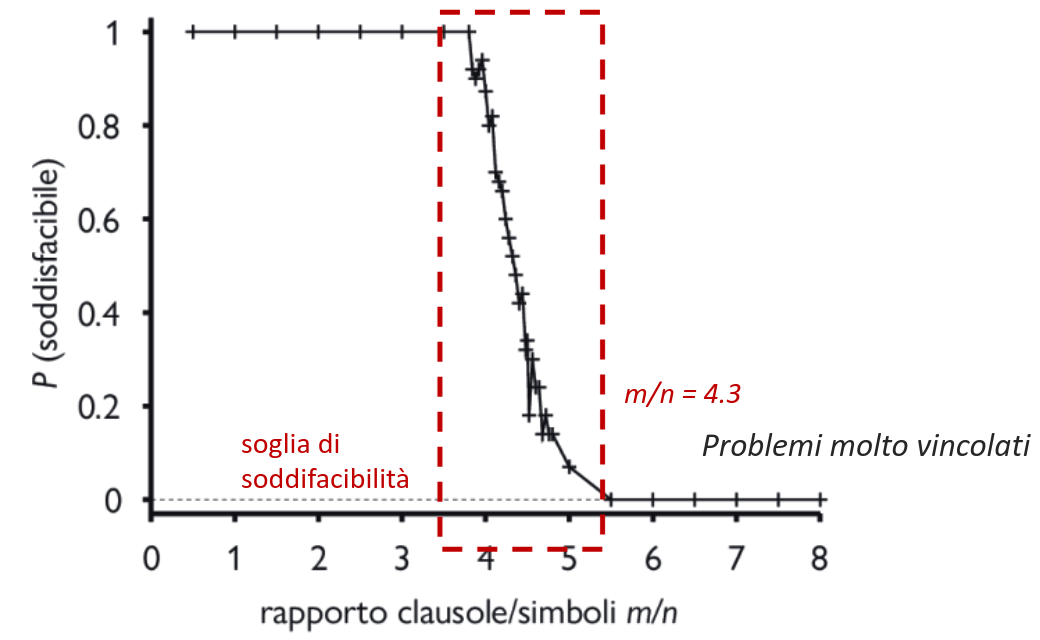
\includegraphics[scale=0.2]{prob_sodd.png}
	\end{center}
	Su 100 problemi generati a caso vediamo che $4.3$ è la soglia oltre la quale un problema diventa difficile da risolvere.
\end{example}
\noindent Vediamo il \textbf{confronto} tra l'algoritmo \hyperref[alg:dpll]{DPLL} e \hyperref[alg:walksat]{WalkSAT}:
\begin{center}
	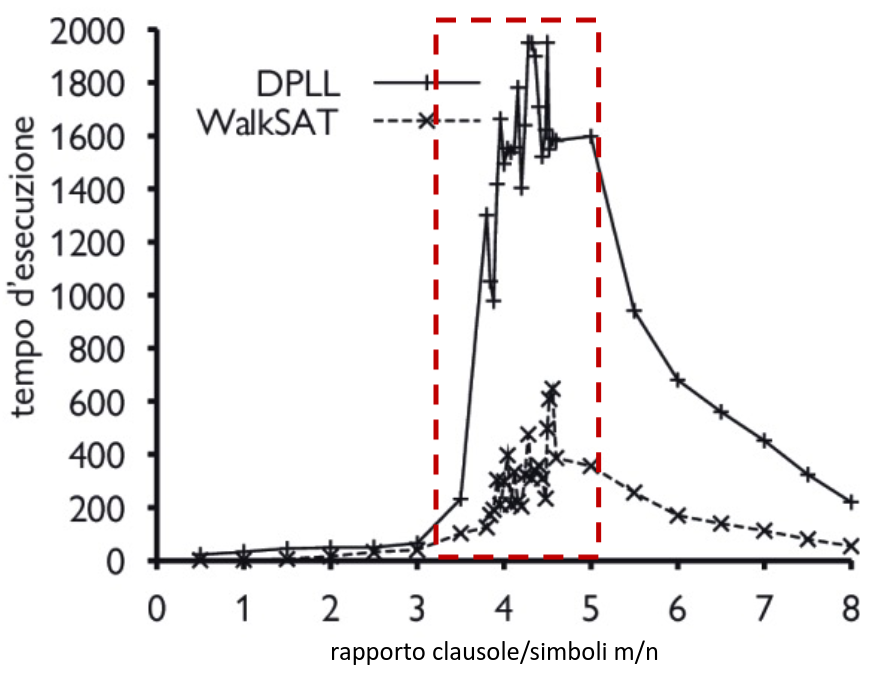
\includegraphics[scale=0.3]{dpll_vs_walksat.png}
\end{center}
Notiamo che i problemi vicini alla \textit{soglia di soddisfacibilità} sono molto più difficili da risolvere rispetto a quelli più lontani. Inoltre vediamo che quando un problema è poco vincolato i due algoritmi performano allo stesso modo mentre intorno alla soglia \textit{WalkSAT} è nettamente migliore.
	% !TeX spellcheck = it_IT
\newpage
\section{Logica proposizionale}
\subsection{Sintassi}
La sintassi è la seguente, rappresentata in BNF:
\begin{equation}
	\begin{split}
		formula & \to formulaAtomica \vert formulaComplessa \\
		formulaAtomica & \to True \vert False \vert simbolo \\
		simbolo & \to P \vert Q \vert R \vert \ldots \\
		formulaComplessa & \to \neg formula \\
		&\vert (formula \land formula) \\
		& \vert (formula \lor formula)\\
		& \vert (formula \Rightarrow formula)\\
		& \vert (formula \Leftrightarrow formula)
	\end{split}
\end{equation}

\subsection{Semantica}
La logica proposizionale segue una semantica \textbf{composizionale}, dove il significato di una frase è determinato dal significato dei suoi componenti a partire dai \textit{simboli proposizionali}. Di seguito la ravola di verità:
\begin{table}[h!]
	\centering
	\begin{tabular}{|cc|ccccc|}
		\hline
		$P$ & $Q$ & $\neg P$ & $P \land Q$ & $P \lor Q$ & $ P \Rightarrow Q$ & $P \Leftrightarrow Q$\\
		\hline
		false & false & true & false & false & true & true \\
		false & true & true & false & true & true & false \\
		true & false & false & false & true & false & false \\
		true & true & false & true & true & true & true\\
		\hline
	\end{tabular}
\end{table}

\subsection{Conseguenza logica}
\begin{definition}[Conseguenza logica]
	Una formula $\alpha$ è una conseguenza logica di un insieme di formule KB se e solo se in ogni modello di KB, anche $\alpha$ è vera ($KB \models \alpha$).
\end{definition}
Indichiamo con $M(KB)$ i modelli dell'insieme di formule in KB e con $M(\alpha)$ l'insieme delle interpretazioni che rendono $\alpha$ vera, ovvero i suoi \textbf{modelli}.
\begin{equation}
	KB \models \alpha \Leftrightarrow M(KB) \subseteq M(\alpha)
\end{equation}

\subsubsection{Model checking}
Un modo per determinare la conseguenza logica è quello di enumere i \textit{modelli} e mostrare che la formula $\alpha$ vale in tutti quelli in cui è vera la KB.

\begin{example}[Wumpus World]
	\label{example:wumpus_world_model_checking}
	Partendo dall'esempio \ref{example:wumpus_world} abbiamo che la KB iniziale, $KB_0$, è costituita dalle regole descritte nella definizione dell'esercizio:
	\begin{gather*}
		\neg W_{1,1} \quad \neg P_{1,1} \\
		B_{2,1} \Leftrightarrow (P_{1,1} \lor P_{2,2,} \lor P_{3,1})\\
		B_{1,1} \Leftrightarrow (P_{1,2} \lor P_{2,1})\\
		\vdots
	\end{gather*}
	Il primo passo dell'agente è spostarsi in $[2,1]$ dato che in $[1,1]$ non ha percepito niente. Abbiamno quindi:
	\begin{equation*}
		KB_1 = KB_0 \cup \{\neg B_{1,1}, B_{2,1}, \neg F_{1,1}, \neg F_{2,1}, \ldots\}
	\end{equation*}
	e rappresentiamo le domande sulla presenza o meno di pozzi come:
	\begin{equation*}
		\begin{split}
			KB_1 \models \neg P_{1,2} \\
			KB_1 \models \neg P_{2,2} \\
			KB_1 \models \neg P_{3,1} \\
		\end{split}
	\end{equation*}
	Sapendo da $KB_0$ che non ci sono pozzi nella casella $[1,1]$ e che c'è un pozzo nella stanza adiacente solo se ci percepisce la brezza, formuliamo le seguenti proposizioni:
	\begin{equation*}
		\begin{split}
			& B_{1,1} \Leftrightarrow (P_{1,2} \lor P_{2,1}) \\
			& B_{2,1} \Leftrightarrow (P_{1,1} \lor P_{2,2} \lor P_{3,1})
		\end{split}
	\end{equation*}
	e concludiamo che non c'è brezza in $[1,1]$ e c'è in $[2,1]$, ovvero $\neg B_{1,1}$ e $B_{2,1}$.\\
	Ci rimangono quindi tre configurazioni possibili dato che abbiamo:
	\begin{gather*}
		KB_1 \models \neg P_{1,2}\\
		KB_1 \models P_{2,2}\lor P_{3,1}
	\end{gather*}
	e sono quelle in cui i pozzi sono in $[3,1]$ oppure in $[2,2]$ oppure in entrambi.i
\end{example}

\subsubsection{SAT}
Un altro approccio alla dimostrazione della conseguenza logica si basa su tre principi:
\begin{itemize}
	\item \textbf{Equivalenza logica}: due formule $\alpha$ e $\beta$sono equivalenti se sono vere nello stesso insieme di modelli
	\begin{equation}
		\alpha \equiv \beta \Leftrightarrow \alpha \models \beta\land\beta\models\alpha
	\end{equation}
	Alcune leggi fondamentali per l'equivalenza sono:
	\begin{itemize}
		\item \textit{Commutatività}: $(\alpha\land\beta)\equiv(\beta\land\alpha)\quad(\alpha\lor\beta)\equiv(\beta\lor\alpha)$
		\item \textit{Associatività}: $((\alpha\land\beta)\land\gamma)\equiv(\alpha\land(\beta\land\gamma))\quad((\alpha\lor\beta)\lor\gamma)\equiv(\alpha\lor(\beta\lor\gamma))$
		\item \textit{Eliminazione della doppia negazione}: $\neg(\neg\alpha)$
		\item \textit{Contrapposizione}: $(\alpha\Rightarrow\beta)\equiv(\neg\beta\Rightarrow\neg\alpha)$
		\item \textit{Eliminazione dell'implicazione}: $(\alpha\Rightarrow\beta)\equiv(\neg\alpha\lor\beta)$
		\item \textit{Eliminazione del bicondizionale}: $(\alpha\Leftrightarrow\beta)\equiv((\alpha\Rightarrow\beta)\land(\beta\Rightarrow\alpha))$
		\item \textit{De Morgan}: $\neg(\alpha \land\beta)\equiv(\neg\alpha\lor\neg\beta)\quad\neg(\alpha \lor\beta)\equiv(\neg\alpha\land\neg\beta)$
		\item \textit{Distributività}: $(\alpha\land(\beta\lor\gamma))\equiv((\alpha\land\beta)\lor(\alpha\land\gamma)\quad(\alpha\lor(\beta\land\gamma))\equiv((\alpha\lor\beta)\land(\alpha\lor\gamma))$
	\end{itemize}
	\item \textbf{Validità}: una formula $\alpha$ è valida se e solo se è vera in tutte le sue interpretazioni. In quel caso sono anche dette \textbf{tatutologie}.
	\begin{theorem}[Teorema di deduzione e refutazione]
		Date due formule $\alpha$ e $\beta$, allora $\alpha \models\beta \Leftrightarrow (\alpha\Rightarrow\beta)$. Possiamo riscriverlo, usando le leggi appena elencate, anche come $\alpha\models\beta \Leftrightarrow (\alpha \land \neg\beta)$, che ci permette di fare la dimostrazione per \textbf{assurdo}.
	\end{theorem}
	\item \textbf{Soddisfacibilità}: una formula $\alpha$ è soddisfacibile se e solo se esiste una interpretazione in cui $\alpha$ è vera (ovvero se esiste un modello di $\alpha$). La determinazione della soddisfacibilità è il problema \textbf{SAT}.
\end{itemize}
Si noti che \textit{validità} e \textit{soddisfacibilità} sono connesse:
\begin{itemize}
	\item $\alpha$ è valida se e solo se $\neg\alpha$ è insoddisfacibile
	\item $\alpha$ è soddisfacibvile se e solo se $\neg\alpha$ non è valida
\end{itemize}
\begin{definition}[Forma a clausole]
	La forma a clausole è la \textbf{forma normale congiuntiva} (CNF), ovvero una congiunzione di disgiunzioni di letterali (un simbolo o la sua negazione). È sempre possibile ottenerla con trasformazioni che preservano l'equivalenza logica.
\end{definition}
Per eseguire una trasformazione in forma a clausole bisogna seguire i seguenti passi:
\begin{enumerate}
	\item Eliminazione del $\Leftrightarrow$
	\item Eliminazione del $\Rightarrow$
	\item Portare le negazioni all'interno tramite De Morgan
	\item Distribuire $\lor$ su $\land$
\end{enumerate}

\begin{example}
	Partendo dall'esempio \ref{example:wumpus_world}, trasformiamo $B_{1,1} \Leftrightarrow (P_{1,2}\lor P_{2,1})$:
	\begin{enumerate}
		\item $(B_{1,1} \Rightarrow (P_{1,2} \lor P_{2,1})) \land ((P_{1,2} \lor P_{2,1}) \Rightarrow B_{1,1})$
		\item $(\neg B_{1,1} \lor (P_{1,2} \lor P_{2,1})) \land (\neg(P_{1,2} \lor P_{2,1}) \lor B_{1,1})$
		\item $(\neg B_{1,1} \lor (P_{1,2} \lor P_{2,1})) \land ((\neg P_{1,2} \land \neg P_{2,1}) \lor B_{1,1})$
		\item $(\neg B_{1,1} \lor P_{1,2} \lor P_{2,1}) \land (\neg(P_{1,2} \lor B_{1,1}) \land (\neg P_{2,1} \lor B_{1,1})$
	\end{enumerate}
	che possiamo riscrivere come
	\begin{equation*}
		\{\neg B_{1,1}, P_{1,2}, P_{2,1}\}\{\neg P_{1,2}, B_{1,1,}\}\{\neg P_{2,1}, B_{1,1}\}
	\end{equation*}
\end{example}

\subsubsection{Deduzione}
Un altro modo per dimostrare la conseguenza logica è utilizzare un \textbf{sistema di deduzione}, che denotiamo come $KB \vdash A$. La deduzione avviene specificando delle \textbf{regole di inferenza} con le seguenti caratteristiche:
\begin{itemize}
	\item Devono derivare \textbf{solo} formule che sono conseguenza logica
	\item Devono derivare \textbf{tutte} le formule che sono conseguenza logica
\end{itemize}
\begin{definition}[Correttezza]
	Tutto ciò che è derivabile è conseguenza logica, le regole preservano la verità.
	\begin{equation}
		KB \vdash \alpha \Rightarrow KB \models \alpha
	\end{equation}
\end{definition}
\begin{definition}[Completezza]
	Tutto ciò che è conseguenza logica è ottenibile tramite il sistema di deduzione.
	\begin{equation}
		KB \models \alpha \Rightarrow KB \vdash \alpha
	\end{equation}
\end{definition}
Alcune regole di inferenza sono:
\begin{gather}
	\frac{\alpha \Rightarrow \beta, \quad \alpha}{\beta} \quad\quad\text{Modu ponens}\\
	\frac{\alpha \land \beta}{\alpha} \quad\quad\text{Eliminazione dell\'AND}\\
	\frac{\alpha \Leftrightarrow \beta}{(\alpha \Rightarrow \beta) \land (\beta \Rightarrow \alpha)} \quad\quad\text{Introduzione della doppia implicazione}\\
	\frac{(\alpha \Rightarrow \beta) \land (\beta \Rightarrow \alpha)}{\alpha \Leftrightarrow \beta} \quad\quad\text{Eliminazione della doppia implicazione}
\end{gather}

\begin{example}[Wumpus]
	Partendo dalle stesse assunzioni fatte nell'esempio \ref{example:wumpus_world_model_checking}, voglio chiedermi se posso dimostrare con le regole di inferenza che non c'è un pozzo in $[1,1]$, ovvero $\neg P_{1,2}$.
	\begin{align*}
		R_6: (B_{1,1} \Rightarrow (P_{1,2} \lor P_{2,1})) \land ((P_{1,2} \lor P_{2,1}) \Rightarrow B_{1,1}) && (R_2, \Leftrightarrow E) \\
		R_7: (P_{1,2} \lor P_{2,1}) \Rightarrow B_{1,1} && (R_6,\land E)\\
		R_8: \neg B_{1,1} \Rightarrow \neg (P_{1,2} \lor P_{2,1}) && (R_7, \text{contrapposizione}) \\
		R_9: \neg(P_{1,2} \lor P_{2,1}) && (R_4, R_8, \text{Modus ponens}) \\
		R_{10}: \neg P_{1,2} \land \neg P_{2,1} && (R_9, \text{De Morgan})\\
		R_{11}: \neg P_{1,2} && (R_10, \land E)
	\end{align*}
\end{example}
\noindent Anche la deduzione può quindi essere visto come problema di ricerca, dove vanno definite:
\begin{itemize}
	\item \textbf{Direzione} della ricerca: nella dimostrazione di teoremi conviene procedere all'\textit{indietro}
	\item \textbf{Strategia} della ricerca:
	\begin{itemize}
		\item \textit{Completezza}: le regole della deduzione naturale sono un un insieme completo, se lo è anche l'algoritmo siamo a posto
		\item \textit{Efficienza}: è un problema decidibile ma NP-Completo
	\end{itemize}
\end{itemize}
In generale per risolvere una proposizione meno regole abbiamo e meglio è, senza però rinunciare alla completezza.\\
Dati $l$ e $m$ letterali positivi o negativi e $l_i$ e $m_j$ di segno opposto, la regola di risoluzione possiamo scriverla in generale come:
\begin{equation}
	\frac{\{l_1, \ldots, l_i, \ldots, l_k\}\{m_1, \ldots, m_j, \ldots, m_n\}}{\{l_1, \ldots, l_{i-1}, l_{i+1}, \ldots, l_k\}\{m_1, \ldots, m_{j-1}, m_{j+1}, \ldots, m_n\}}
\end{equation}
da cui poi possiamo costruirci un \textbf{grafo di risoluzione}.

\newpage
\subsection{Algoritmi}
Di seguito alcuni algoritmi per determinare se è vera una conseguenza logica a partire da una KB.
\subsubsection{TV-Consegue}
Questo algoritmo enumera tutte le possibili interpretazioni di KB, e per ciascuna interpretazione se soddisfa la KB controlla che soddisfi anche $\alpha$. Basta trovare una singola interpretazione che soddisfa la KB ma non $\alpha$ per determinare una risposta negativa. Avremo quindi, dati $k$ simboli, $2^k$ possibili interpretazioni.
\label{alg:tv_consegue}
\begin{lstlisting}
	function TV-Consegue?(KB, a) // Restituisce true oppure false
	inputs: KB, la base di conoscenza, una formula della logica proposizionale
	a, la query, una formula della logica proposizionale
	simboli = una lista dei simboli proposizionali contenuti in KB e a
	return TV-Verifica-Tutto(KB, a, simboli, { })
	
	function TV-Verifica-Tutto(KB, a, simboli, modello) // Restituisce true oppure false
	if Vuoto?(simboli) then
	if PL-Vero?(KB, modello) then return PL-Vero?(a, modello)
	else return true // Quando KB false, restituisce sempre true
	else do
	P = Primo(simboli); resto = Resto(simboli)
	return TV-Verifica-Tutto(KB, a, resto, modello = {P = true})
	and
	TV-Verifica-Tutto(KB, a, resto, modello = {P = false})
\end{lstlisting}

\begin{example}
	Supponiamo di voler verificare la seguente conseguenza logica:
	\begin{equation*}
		(\neg a\lor b)\land(a \lor c) \models (b \lor c)
	\end{equation*}
	Ci costruiamo la tabella di verità:
	\begin{table}[!h]
		\centering
		\begin{tabular}{|ccc|cc|}
			\hline
			$a$&$b$&$c$&$\neg a \lor b$ & $a \lor c$ \\
			\hline
			T & T & T & T & T\\
			T & T& F & T & T \\
			T & F &T&F&T\\
			T&F&F&F&T\\
			F&T&T&T&T\\
			F&T&F&T&F\\
			F&F&T&T&T\\
			F&F&F&T&F\\
			\hline
		\end{tabular}
	\end{table}
	Per poi selezionare solo le righe in cui la KB è vera e verificare se la nostra formula è sempre vera:
	\begin{table}[!h]
		\centering
		\begin{tabular}{|ccc|cc|c|}
			\hline
			$a$&$b$&$c$&$\neg a \lor b$ & $a \lor c$ & $b\lor c$\\
			\hline
			T & T & T & T & T & T\\
			T & T& F & T & T & T\\
			F&T&T&T&T & T\\
			F&F&T&T&T&T\\
			\hline
		\end{tabular}
	\end{table}
	Quindi la risposta è sì.\\
	Applicando l'algoritmo \ref{alg:tv_consegue} abbiamo la seguente esecuzione:
	\begin{lstlisting}
		TV-VERIFICA-TUTTO(KB, formula, [a, b, c], { })
		TV-VERIFICA-TUTTO(KB, formula, [b, c], {a=T})
		TV-VERIFICA-TUTTO(KB, formula, [c], {a=T, b=T})
		TV-VERIFICA-TUTTO(KB, formula, [ ], {a=T, b=T, c=T}) // OK
		TV-VERIFICA-TUTTO(KB, formula, [ ], {a=T, b=T, c=F}) // OK
		TV-VERIFICA-TUTTO(KB, formula, [c], {a=T, b=F})
		TV-VERIFICA-TUTTO(KB, formula, [ ], {a=T, b=F, c=T}) // OK
		TV-VERIFICA-TUTTO(KB, formula, [ ], {a=T, b=F, c=F}) // OK
		TV-VERIFICA-TUTTO(KB, formula, [b, c], [a=F])
		etc...
	\end{lstlisting}
\end{example}
\subsubsection{DPLL}
\label{alg:dpll}
Questo algoritmo parte da una KB in forma a clausole e prende in input una formula in CNF ed enumera ricorsivamente in profondità tutte le possibili interpretazioni alla ricerca di un modello. Per avere un miglioramento sull'algoritmo \ref{alg:tv_consegue} applico tre clausole:
\begin{itemize}
	\item \textbf{Terminazione anticipata}: si può decidere sulla verità di una clausola anche con interpretazioni parziali, ovvero quando ho degli \textit{OR} basta che un simbolo sia vero mentre quando ho degli \textit{AND} basta che unpo sia falso per rendere falsa l'intera interpretazione
	\item \textbf{Euristica dei simboli puri}: un simbolo puro è un simbolo che appare con lo stesso segno in tutte le clausole (trascurando eventualmente quelle già rese vere). Possono poi essere assegnati a True se il letterale è positivo o a False se è negativo
	\item \textbf{Euristica delle clausole unitarie}: una clausola in cui è rimasto un solo letterale non assegnato
\end{itemize}

\begin{lstlisting}
	function DPLL-Soddisfacibile?(s) returns true oppure false
	inputs: s, una formula della logica proposizionale
	clausole = insieme di clausole nella rappresentazione CNF di s
	simboli = una lista di tutti i simboli proposizionali in s
	return DPLL(clausole, simboli, { })
	
	function DPLL(clausole, simboli, modello) returns true oppure false
	if ogni clausola in clausole vera in modello then return true
	if qualche clausola in clausole falsa in modello then return false
	P, valore = Trova-Simbolo-Puro(simboli, clausole, modello)
	if P diverso da null then return DPLL(clausole, simboli - P, modello = {P = valore})
	P, valore = Trova-Clausola-Unitaria(clausole, modello)
	if P diverso da null then return DPLL(clausole, simboli-P, modello = {P = valore})
	P = Primo(simboli); resto = Resto(simboli)
	return	DPLL(clausole, resto, modello = {P = true})
	or
	DPLL(clausole, resto, modello = {P = false})
\end{lstlisting}

\begin{example}
	Supponiamo di voler verificare la seguente conseguenza logica:
	\begin{equation*}
		\{\neg B_{1,1}, P_{1,2}, P_{2,1}\}\{\neg P_{1,2}, B_{1,1}\}\{\neg P_{2,1}, B_{1,1}\}\{\neg B_{1,1}\} \models \{\neg P_{1,2}\}
	\end{equation*}
	Aggiungiamo alla KB la clausola $\{P_{1,2}\}$ e verifichiamo con SAT se l'insieme è insoddisfacibile:
	\begin{enumerate}
		\item La clausola $\{P_{1,2}\}$ è unitaria, quindi $P_{1,2}=True$. Di conseguenza $\{\neg B_{1,1}, P_{1,2}, P_{2,1}\}$ e $\{P_{1,2}\}$ sono soddisfatte e rimaniamo con
		\begin{equation*}
			\{\neg P_{1,2}, B_{1,1}\}\{\neg P_{2,1}, B_{1,1}\}\{\neg B_{1,1}\}
		\end{equation*}
		\item $P_{2,1}$ è un simbolo puro ed essendo negativo sarà uguale a False, quindi la clausola $\{\neg P_{2,1}, B_{1,1}\}$ è soddisfatta e rimaniamo con
		\begin{equation*}
			\{\neg P_{1,2}, B_{1,1}\}\{\neg B_{1,1}\}
		\end{equation*}
	\end{enumerate}
	Dato che non esistono modelli possiamo dire che $\neg P_{1,2}$ è conseguenza logica della KB
\end{example}
\noindent Questo algoritmo è \textbf{completo} e \textbf{termina sempre}. Alcuni miglioramenti sono:
\begin{itemize}
	\item Se possibile scomporre in sotto problemi indipendenti (quando non hanno simboli in comune)
	\item Ordinare le variabili per frequenza di comparizione
	\item Backtracing intelligente
\end{itemize}

\subsubsection{WalkSAT}
\label{alg:walksat}
Definiamo la formulazione di un problema SAT in ambito locale:
\begin{itemize}
	\item \textbf{Stati}: sono le interpretazioni, assegnamenti completi
	\item \textbf{Obiettivo}: un assegnamento che soddisfa tutte le clausole (\textit{modello})
\end{itemize}
Si parte da un assegnamento \textit{casuale} e ad ogni passo si cambia il valore di un simbolo proposizionale (\textbf{flip}). La valutazione di uno stato avviene controllando il numero di clausole soddisfatte.

Ad ogni passo viene scelta a caso una clausola non soddisfatta e individua un simbolo da modificare, scegliendo con probabilità $p$ tra:
\begin{itemize}
	\item \textbf{Random walk}: il simbolo è scelto a caso
	\item \textbf{Ottimizzazione}: viene scelto il simbolo che rende più clausole soddisfatte
\end{itemize}
Dopo un certo numero di flip predefinito, l'algoritmo si arrende.
\begin{lstlisting}
	function WalkSAT(clausole, p, max_flips) returns un modello o fallimento
	modello = assegnamento casuale di valori di verita ai simboli in clausole
	
	for i = 1 to max_flips do
	if modello soddisfa clausole then return modello
	clausola = una clausola, falsa in modello, scelta casualmente nell'insieme clausole
	if Random(0, 1) =< p then inverti il valore in modello di un simbolo scelto
	casualmente in clausola
	else inverti il valore di verita del simbolo in clausole che massimizza il numero
	di clausole soddisfatte
	
	return fallimento
\end{lstlisting}

\begin{example}[WalkSAT]
	L'obiettivo è quello di massimizzare il numero di clausole soddisfatte tra le seguenti:
	\begin{equation*}
		\{\neg B_{1,1}, P_{1,2}, P_{2,1}\}\{\neg P_{1,2}, B_{1,1}\}\{\neg P_{2,1}, B_{1,1}\}\{\neg B_{1,1}\}
	\end{equation*}
	Un esempio di esecuzione dell'algoritmo è il seguente:
	\begin{enumerate}
		\item Configurazione di \textit{partenza}: $[B_{1,1}=F,P_{1,2}=T,P_{2,1}=T]$
		\item \textit{Random walk}: la prima e la quarta clausola sono soddisfatte, scelgo seconda e faccio un flip a caso di $B_{1,1}$ ottenendo $[B_{1,1}=T,P_{1,2}=T,P_{2,1}=T]$
		\item L'unica non soddisfatta è la quarta, posso solo fare un flip di $B_{1,1}$ ottenendo $[B_{1,1}=F,P_{1,2}=T,P_{2,1}=T]$
		\item \textit{Random walk}: la prima e la quarta clausola sono soddisfatte, scelgo la seconda e faccio un flip a caso di $P_{1,2}$ ottenendo $[B_{1,1}=F,P_{1,2}=F,P_{2,1}=T]$
		\item \textit{Ottimizzazione}: l'unica non soddisfatta è la terza, faccio un flip di $P_{2,1}$ ottenendo $[B_{1,1}=F,P_{1,2}=F,P_{2,1}=F]$
	\end{enumerate}
\end{example}

Se il limite $max_flips = \infty$ e l'insieme di clausole è soddisfacibile, prima o poi termina, ma  se non lo è non terminerà mai. Non possiamo quindi usarlo per verificare l'insoddisfacibilità.

\subsubsection{Confronto}
Se un problema è \textbf{sotto-vincolato} (ha molte soluzioni) è più probabile che \textit{WalkSAT} trovi una soluzione in tempi brevi.
\begin{example}[3-SAT]
	Dato il seguente problema 3-SAT, ovvero con clausole di 3 letterali:
	\begin{equation*}
		\{\neg D, \neg B, C\} \{B, \neg A, \neg C\} \{\neg C, \neg B, E\} \{E, \neg D, B\} \{B, E, \neg C\}
	\end{equation*}
	Abbiamo $32$ possibili interpretazioni con $16$ possibili soluzioni. Questo sarebbe facile da risolvere con \textit{Walk-SAT}.
\end{example}
\noindent È importante nel capire il livello di difficoltà di un problema SAT il rapporto tra numero di \textbf{clausole} e numero di \textbf{simboli}
\begin{equation}
	\frac{m}{n}
\end{equation}
Infatti, più è grande il rapporto e più vincolato è il problema.
\begin{example}
	Supponiamo di avere $n=50$ simboli e di avere $m$ clausole che variano.
	\begin{center}
		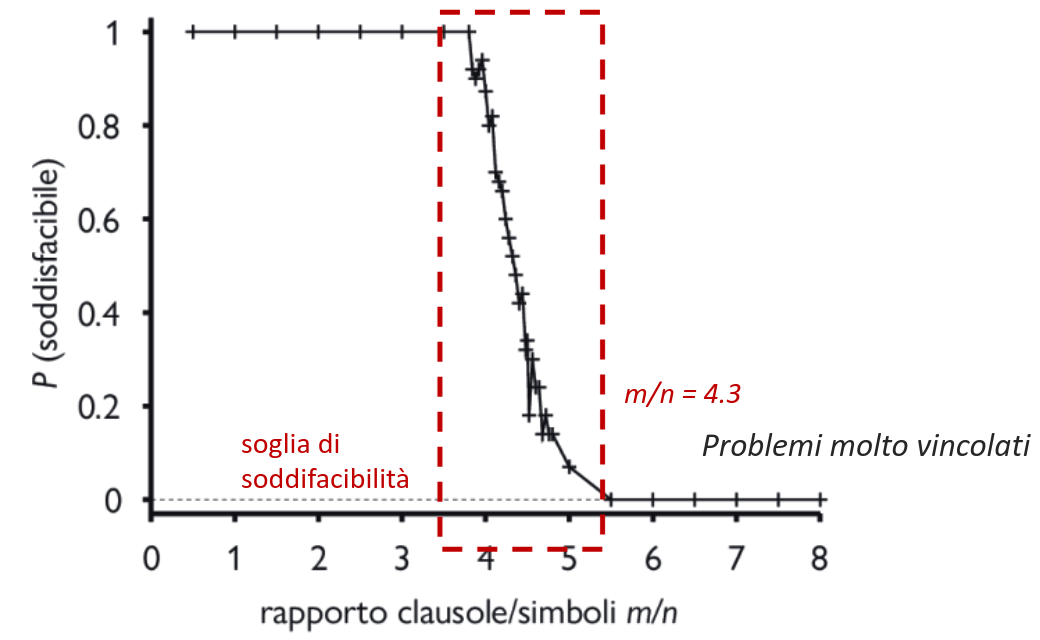
\includegraphics[scale=0.2]{prob_sodd.png}
	\end{center}
	Su 100 problemi generati a caso vediamo che $4.3$ è la soglia oltre la quale un problema diventa difficile da risolvere.
\end{example}
\noindent Vediamo il \textbf{confronto} tra l'algoritmo \hyperref[alg:dpll]{DPLL} e \hyperref[alg:walksat]{WalkSAT}:
\begin{center}
	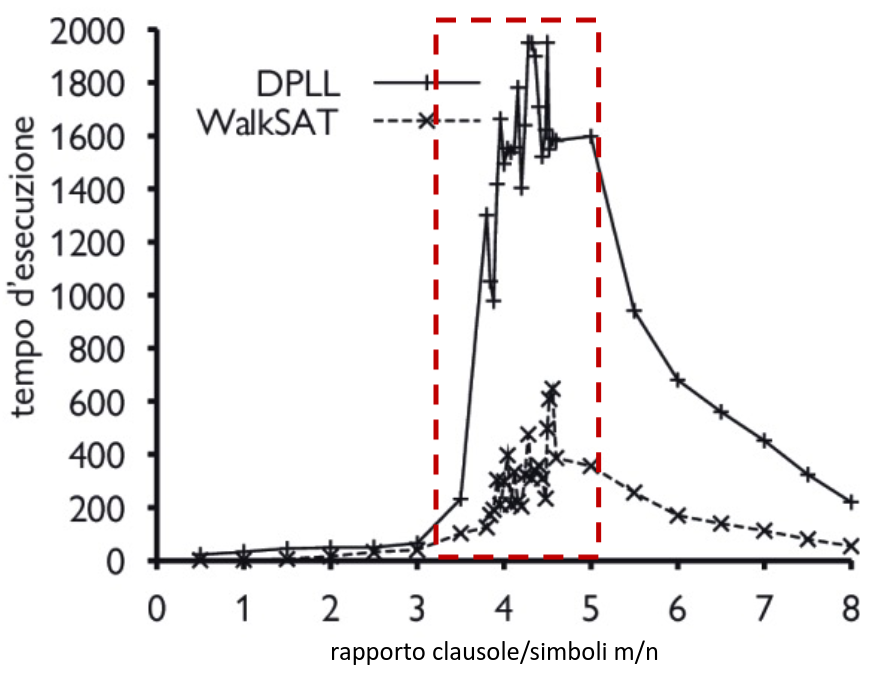
\includegraphics[scale=0.3]{dpll_vs_walksat.png}
\end{center}
Notiamo che i problemi vicini alla \textit{soglia di soddisfacibilità} sono molto più difficili da risolvere rispetto a quelli più lontani. Inoltre vediamo che quando un problema è poco vincolato i due algoritmi performano allo stesso modo mentre intorno alla soglia \textit{WalkSAT} è nettamente migliore.
	% !TeX spellcheck = it_IT
\newpage
\section{Logica del prim'ordine}
Il problema principale della logica proposizionale è che non ha la potenza espressiva per descrivere un ambiente con molti oggetti in modo conciso. Nella logica del prim'ordine abbiamo assunzioni più ricche riguardo la natura della realtà: \textit{oggetti}, \textit{relazioni}, \textit{proprietà}.\\

\subsection{Concettualizzazione}
Il primo passo è quello di decidere quali sono le cose di cui vogliamo parlare, dobbiamo quindi definire gli \textbf{oggetti}, che possono essere identificati da \textit{simboli} o da \textit{funzioni} che li mettono in relazione con altri oggetti. L'insieme degli oggetti rilevanti costituiscono il \textbf{dominio del discorso}, che potrebbe anche essere infinito.\\
Ci sono poi le \textbf{relazioni}, le \textbf{proprietà} (unarie) e le funzioni (biettive).

\begin{example}[Mondo dei blocchi]
	Siamo in un mondo di blocchi, che ad esempio può essere strutturato nel seguente modo:
	\begin{center}
		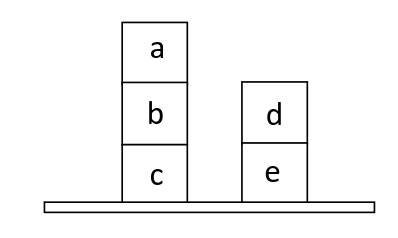
\includegraphics[scale=0.2]{block_world.png}
	\end{center}
	Per prima cosa definiamo il \textit{dominio} composto dai blocchi presenti:
	\begin{equation*}
		\{a,b,c,d,e\}
	\end{equation*}
	Poi individuiamo le \textit{funzioni} rilevanti ad identificare gli oggetti, nel nostro caso solo quella che, dato un blocco, identifica quello che ci sta sopra:
	\begin{equation*}
		Hat(b)=a
	\end{equation*}
	Infine abbiamo le \textit{relazioni}:
	\begin{gather*}
		On=\{<a,b>,<b,c>,<d,e>\} \\
		Clear=\{a,d\}\\
		Table=\{c,e\}\\
		Block=\{a,b,c,d,e\}
	\end{gather*}
	Riassumiamo la nostra \textbf{concettualizzazione} come la seguente tupla composta da \textit{dominio}, \textit{funzioni} e \textit{relazioni}:
	\begin{equation*}
		<\{a,b,c,d,e\}, \{Hat\}, \{On, Clear, Table, Block\}>
	\end{equation*}
\end{example}

\subsection{Sintassi}
\subsubsection{Simboli}
Gli elementi sintattici di base sono i simboli usati per indicare oggetti, relazioni e funzioni. Ne abbiamo di tre tipi:
\begin{itemize}
	\item \textbf{Simboli di costante}: rappresentano gli oggetti
	\item \textbf{Simboli di predicato}: rappresentano le relazioni
	\item \textbf{Simboli di funzione}: rappresentano le funzioni
\end{itemize}
Ogni simbolo degli ultimi due tipi ha una specifica \textbf{arità}, che ne indica il numero di \textit{argomenti}.\\
Quando gli oggetti non sono specificati, usiamo le \textbf{variabili}, che ci consentono di formulare predicati che possono essere veri o falsi a seconda di che valore assegnamo.

\subsubsection{Termini}
Un termine è un'espressione logica che si riferisce ad un oggetto. Ha la seguente sintassi:
\begin{equation*}
	Termine \to Costante \vert Variabile \vert Funzione(Termine, \ldots)
\end{equation*}
\begin{example}
	Alcuni esempi di termini ben formati:
	\begin{gather*}
		f(x,y) \quad +(2,3) \quad Padre-di(Giovanni) \\
		x,A,B,2 \quad Prezzo(Banane) \quad Hat(A)
	\end{gather*}
\end{example}

Il simbolo di \textbf{uguaglianza} si usa per dire che due termini fanno \textit{riferimento} allo stesso oggetto:
\begin{equation*}
	\exists x,y \quad Fratello(x, Riccardo)\land Fratello(y, Riccardo) \land \neg (x=y)
\end{equation*}

\subsubsection{Formule}
Una formula \textbf{atomica} è l'espressione più semplice e \textit{indivisibile} che afferma una relazione tra oggetti del dominio. È composta da un \textit{predicato} seguito da una \textit{lista di termini} che corrispondono alla sua arità. Le formule atomiche non contengono quantificatori, connettivi logici o altre formule come componenti. Ha la seguente sintassi:
\begin{align*}
	\text{Formula-atomica} \rightarrow & True \vert False \vert \\
	& \text{Termine} = \text{Termine } \vert\\
	& \text{Predicato}(\text{Termine}, \ldots)
\end{align*}
Ci sono poi le formule \textbf{complesse}, nelle quali possiamo usare \textit{connettivi logici} e \textit{quantificatori}. Hanno la seguente sintassi:
\begin{align*}
	\text{Formula} \rightarrow & \text{Formula-atomica } \vert \\
	& \text{Formula} \quad \text{Connettivo} \quad \text{Formula } \vert \\
	& \text{Quantificatore} \quad \text{Variabile} \quad \text{Formula } \vert \\
	& \neg \text{Formula } \vert (\text{Formula})
\end{align*}

\begin{example}
	Alcune formule \textit{atomiche} ben formate:
	\begin{gather*}
		Ama(Giorgio, Lucia) \quad On(A,B) \quad Madre-di(Luigi) = Silvana \\
		Amico(Padre-di(Giorgio), Padre-di(Elena)) \quad +(2,3)=5 \quad x=5
	\end{gather*}
	Alcune formule \textit{complesse} ben formate:
	\begin{gather*}
		On(A,B) \land On(B,C) \\
		Studia(Paolo) \Rightarrow Promosso(Paolo)
	\end{gather*}
\end{example}

\subsubsection{Quantificatori}
Esistono due tipi di quantificatori:
\begin{itemize}
	\item \textbf{Universale}: la relazione si applica a tutti gli elementi del dominio (e.g. $\forall x \quad Ama(x, Gelato)$)\\
	\item \textbf{Esistenziale}: la relazione si applica ad almeno un elemento del dominio (e.g. $\exists x \quad Mela(x) \land Rossa(x)$)
\end{itemize}
\begin{note}
	L'ordine dei quantificatori è importante.
\end{note}
Ogni quantificatore ha un suo \textbf{scope}, ad esempio nel seguente predicato
\begin{equation*}
	\forall x (\exists y \quad Ama(x,y))
\end{equation*}
$\exists y$ ha come scope $Ama(x,y)$ mentre $\forall x$ ha come scope $(\exists y \quad Ama(x,y))$.
\subsubsection{Linguaggio}
Il linguaggio della logica del prim'ordine è descritto dal seguente vocabolario:
\begin{align*}
	&\text{Connettivo} \rightarrow \land \vert \lor \vert \neg \vert \Rightarrow\vert\Leftrightarrow\vert\Leftarrow \\
	&\text{Quantificatore}\rightarrow\forall\vert\exists\\
	&\text{Variabile}\rightarrow x\vert y \vert \ldots \vert a \vert \ldots \vert s \vert \ldots\\
	&\text{Costante} \rightarrow A \vert B \vert \ldots \vert Mario \vert Pippo \vert \ldots \vert 1 \vert \ldots\\
	&\text{Funzione} \rightarrow Hat \vert Padre-di \vert + \vert - \vert \ldots\\
	&\text{Predicato} \rightarrow On \vert Clear \vert \geq \vert < \vert \ldots
\end{align*}
Quando utilizziamo le variabili nell'ambito dei quantificatori sono definite \textbf{legate}, altrimenti sono \textbf{libere}.

\begin{definition}[Formula chiusa]
	Una formula che non contiene occorrenze di variabili libere.
\end{definition}
\begin{definition}[Formula aperta]
	Una formula che contiene occorrenze di variabili libere.
\end{definition}
\begin{definition}[Formula ground]
	Una formula che non contiene variabili.
\end{definition}

\begin{observation}[Precedenza]
	Nel linguaggio della logica del prim'ordine è importante la precedenza tra gli operatori logici. Ad esempio:
	\begin{align*}
		\forall x \quad Persona(x) \Rightarrow Sesso(x)=M \lor Sesso(x)=F \lor Sesso(x)=NB \\
		\lor  Sesso(x)=GQ \lor Sesso(x)=GF \lor Sesso(x)=A
	\end{align*}
	deve essere interpretata come:
	\begin{align*}
		\forall x \quad (Persona(x) \Rightarrow ((Sesso(x)=M) \lor (Sesso(x)=F) \lor (Sesso(x)=NB) \\
		\lor (Sesso(x)=GQ) \lor (Sesso(x)=GF) \lor (Sesso(x)=A)))
	\end{align*}
\end{observation}

\subsection{Semantica}
La logica del prim'ordine usa una semantica di tipo \textbf{dichiarativo}, che consiste nello stabilire una corrispondenza tra:
\begin{itemize}
	\item I \textit{termini} del linguaggio e gli \textit{oggetti} del mondo
	\item Le \textit{formule chiuse} e i \textit{valori di verità}
\end{itemize}

\subsubsection{Componenti}
Le componenti principali della semantica sono:
\begin{itemize}
	\item \textbf{Universo} del discorso: un insieme non vuoto di elementi che rappresenta l'insieme di tutti gli \textit{oggetti} che si prendono in considerazione
	\item \textbf{Assegnazione di valori}:
	\begin{itemize}
		\item Alle \textit{costanti} si assegna un elemento specifico dell'universo
		\item Alle \textit{variabili} si possono assegnare elementi dell'universo attraverso una \textit{funzione}
		\item Alle \textit{funzioni} si assegna una mappatura da una sequenza di elementi dell'universo ad un singolo elemento dell'universo (rispettando la sua \textit{arità})
		\item Ai \textit{predicati} si assegna una relazione sull'universo (rispettando la sua \textit{arità})
	\end{itemize}
	\item \textbf{Verità di formule}:
	\begin{itemize}
		\item Una formula \textit{atomica} è vera se l'interpretazione assegna ai suoi termini una sequenza che rientra nella relazione specificata dal predicato
		\item Una formula \textit{complessa} viene valutata sulla  base dei suoi componenti usando il significato dei \textit{connettori logici} e dei \textit{quantificatori}
	\end{itemize}
\end{itemize}

\subsubsection{Interpretazione}
Una interpretazione $I$ stabilisce una \textit{corrispondenza} tra elementi atomici del linguaggio ed elementi della concettualizzazione. Interpreta:
\begin{itemize}
	\item I simboli di \textit{costante} come elementi del dominio $D$
	\item I simboli di \textit{funzione} come funzioni da n-uple di $D$ in $D$
	\item I simboli di \textit{predicato} come insiemi di n-unple (relazioni)
\end{itemize}

\begin{example}
	Partiamo da un'altra versione del mondo dei blocchi:
	\begin{center}
		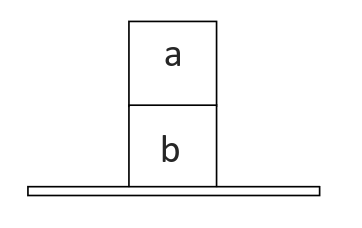
\includegraphics[scale=0.2]{block_world_2.png}
	\end{center}
	concettualizzato come segue:
	\begin{align*}
		On(A,B) \\
		Clear(A) \\
		Table(B)
	\end{align*}
	Una possibile interpretazione è la seguente:
	\begin{align*}
		&I(A)=a \quad I(B)=b \\
		&I(On)=\{<a,b>\}\\
		&I(Clear)=\{a\}\\
		&I(Table)=\{b\}
	\end{align*}
	ma lo è anche:
	\begin{align*}
		&I(A)=a \quad I(B)=b \\
		&I(On)=\{<b,a>\}\\
		&I(Clear)=\{b\}\\
		&I(Table)=\{a\}
	\end{align*}
\end{example}
Quindi il significato di un termine o di una formula composta è determinato in funzione del significato dei suoi componenti.\\
Nel caso dei quantificatori:
\begin{itemize}
	\item \textbf{Universale}: $\forall x \: A(X)$ è vera se lo è per ciascun elemento del dominio di $A$. Se il dominio è \textit{finito} equivale ad una serie di $\land$. Data la forza del quantificatore universale, spesso si restringe il suo campo d'azione mediante $\Rightarrow$
	\item \textbf{Esistenziale}: $\exists x \: A(x)$ e vera se esiste almeno un elemento del dominio per cui $A$ è vera. Se il dominio è \textit{finito} equivale ad una serie di $\lor$. Data la debolezza del quantificatore esistenziale, di solito si usa con $\land$
\end{itemize}
Da questo possiamo derivare alcune proprietà che mettono in relazione i due quantificatori (a destra le proprietà della logica da cui sono derivate):
\begin{align*}
	&\forall x \: \neg P(x) \equiv \neg \exists x \: P(x) & \neg P \land \neg Q \equiv \neg (P \lor Q)\\
	&\neg \forall x \: P(x) \equiv \exists x \: \neg P(x)&\neg(P \land Q) \equiv \neg P \lor \neg Q \\
	&\forall x \: P(x) \equiv \neg \exists x \: \neg P(x) & P \land Q \equiv \neg(\neg P \lor \neg Q)\\
	&\neg \forall x \: \neg P(x) \equiv \exists x \: P(x) & P \lor Q \equiv \neg (\neg P \land \neg Q)
\end{align*}

\begin{note}
	La semantica standard, che segue la logica classica, è spesso molto prolissa anche per esprimere concetti molto semplici. Per combattere questo problema esiste la semantica dei \textbf{database} che parte dalle seguenti ipotesi per essere più concisa:
	\begin{itemize}
		\item \textit{Nomi unici}: simboli e oggetti distinti, ogni costante fa riferimento ad un oggetto distinto
		\item \textit{Mondo chiuso}: tutto ciò di cui non si sa che è vero, è falso, quindi le formule atomiche non conosciute come vere sono false
		\item \textit{Chiusura del dominio}: esistono solo gli oggetti di cui si parla. Ogni modello contiene un numero di elementi del dominio non superiore a quello degli elementi denominati dai simboli di costante
	\end{itemize}
\end{note}
\subsubsection{Knowledge Base}
Le interazioni con la Knowledge Base in logica del prim'ordine sono fatte sfruttando:
\begin{itemize}
	\item \textbf{Asserzioni}, ad esempio
	\begin{equation*}
		TELL(KB, Re(Giovanni))
	\end{equation*}
	\item \textbf{Interrogazioni}, ad esempio
	\begin{equation*}
		ASK(KB, Persona(Giovanni)) \longrightarrow Si
	\end{equation*}
\end{itemize}

\begin{example}[Wumpus World]
	Possiamo implementare l'esempio del Wumpus World (\ref{example:wumpus_world}) in FOL, descrivendo tutto in maniera più precisa. Alcuni casi:
	\begin{itemize}
		\item \textbf{Percezioni}: possiamo rappresentarle come un predicato binario $Percezione(5-upla, t)$
		\item \textbf{Regole} per le percezioni: ad esempio per lo scintillio
		\begin{gather*}
			\forall t,s,b,m,c \: Percezione( [s,b,Scintillio,m,c], t) \Rightarrow Scintillio(t)\\
			\forall t,s,b,m,c \: Percezione( [s,b,None,m,c], t) \Rightarrow \neg Scintillio(t)
		\end{gather*}
		\item Descrizione della \textbf{mappa}: ad esempio l'adiacenza di una casella
		\begin{equation*}
			\forall x,y,a,b \: Adiacente([x,y], [a,b]) \Leftrightarrow (x=a \land(y=b-1 \lor y=b+1)) \lor (y=b \land (x=a-1 \lor x=a+1))
		\end{equation*}
	\end{itemize}
\end{example}

\subsection{Inferenza}
Dobbiamo eliminare i quantificatori. Introduciamo prima il concetto di \textbf{sostituzione}: $A[x/g]$ è il risultato della sostituzione di $g$ per $x$ in $A$.
\subsubsection{Istanziazione}
L'instanziazione \textbf{universale} prevede di inferire tutte le formule ottenute sostituendo un termine \textit{ground} $g$ a una variabile quantificata universalmente $x$.
\begin{equation}
	\frac{\forall x \: A[x]}{A[x/g]}
\end{equation}
\begin{example}
	Data la proposizione
	\begin{equation*}
		\forall x \: Re(x) \land Avido(x) \Rightarrow Malvagio(x)
	\end{equation*}
	si possono ottenere:
	\begin{align*}
		&Re(Giovanni) \land Avido(Giovanni) \Rightarrow Malvagio(Giovanni)\\
		&Re(Padre(Giovanni))  \land Avido(Padre(Giovanni)) \Rightarrow Malvagio(Padre(Giovanni))
	\end{align*}
\end{example}
L'instanziazione \textbf{esistenziale} prevede di sostituire una variabile quantificata esistenzialmente con un unico nuovo simbolo costante.
\begin{equation}
	\frac{\exists x\: A[x]}{A[x/k]}
\end{equation}
Se $\exists$ non compare nello scope di $\forall$, $k$ è una costante nuova chiamata \textbf{costante di Skolem}, altrimenti va introdotta una \textbf{funzione di Skolem} nelle variabili quantificate universalmente. Alcuni esempi:
\begin{align*}
	&\exists x \: Padre(x, G) \longrightarrow Padre(K, G) \\
	&\forall x \exists y \: Padre(x,y) \longrightarrow \forall x \: Padre(x, p(x))
\end{align*}

\subsubsection{Grounding}
La riduzione a inferenza proposizionale è detta \textbf{grounding} e prevede i seguenti passaggi:
\begin{enumerate}
	\item Istanziazione universale
	\item Istanziazione esistenziale
	\item Sostituire le formule \textit{atomiche ground} con simboli proposizionali
\end{enumerate}
Il problema che rimane prima di poter applicare gli algoritmi già visti è che anche se le costanti sono in numero finito, in presenza di funzioni le istanze da creare sono infinite: ad esempio:
\begin{equation*}
	Giovanni, Padre(Giovanni), Padre(Padre(Giovanni)), \ldots
\end{equation*}

\begin{theorem}[Teorema di Herbrand]
	Se $KB \models \alpha$, allora c'è una dimostrazione che coinvolge solo un sotto-insieme finito della KB proposizionalizzata.
\end{theorem}
Per applicare il teorema appena enunciato si può procedere \textit{incrementalmente}:
\begin{enumerate}
	\item Creare le istanza con le costanti
	\item Creare le istanze con un solo livello di annidamento
	\item Procedere livello per livello finché non siamo in grado di costruire la dimostrazione proposizionale della formula che è conseguenza logica
\end{enumerate}
Se $KB\nvDash$ il processo non termina. Il problema è quindi \textbf{semidecidibile}.

\subsubsection{Forma a clausole}
Per estendere alla logica del prim'ordine il metodo di risoluzione dobbiamo prima estendergli anche la trasformazione in forma a clausole.\\
\textit{Costanti}, \textit{funzioni} e predicati sono come definiti ma escludendo formule atomiche del tipo $t_1 = t_2$. Definiamo quindi una clausola come un insieme di \textit{letterali} che rappresenta la loro disgiunzione:
\begin{align}
	& Clausola \rightarrow \{Letterale, \ldots, Letterale\}\\
	& Letterale \rightarrow Formula_atomica \: \vert \: \neg Formula_atomica
\end{align}
Una Knowledge Base è quindi un insieme di clausole.
\begin{theorem}
	Per ogni formula chiusa $\alpha$ del FOL è possibile trovare in maniera \textbf{effettiva}un insieme di clausole $FC(\alpha)$ che è soddisfacibile se e solo se $\alpha$ lo è. Allo stesso modo per l'insoddisfacibilità.
\end{theorem}
\begin{definition}[Effettivo]
	Esiste una procedura che può essere eseguita per trasformare la formula $\alpha$ in un insieme di clausole $FC(\alpha)$ tale che valga questo risultato.
\end{definition}

\begin{example}[Trasformazione in forma a clausole]
	Vediamo passo per passo il processo di trasformazione appena descritto applicato alla frase:
	\begin{equation*}
		\forall x(\forall y \: Animale(y) \Rightarrow Ama(x,y)) \Rightarrow (\exists y \: Ama(y,x))
	\end{equation*}
	\begin{enumerate}
		\item Eliminazione delle implicazioni
		\begin{align*}
			&\forall x \neg(\forall y \: Animale(y) \Rightarrow Ama(x,y)) \lor (\exists y \: Ama(y,x))\\
			&\forall x\neg(\forall y \: \neg Animale(y) \lor Ama(x,y)) \lor (\exists y \: Ama(y,x))
		\end{align*}
		\item Negazioni all'interno
		\begin{align*}
			&\forall x(\exists y \neg (\neg Animale(y) \lor Ama(x,y))) \lor (\exists y \: Ama(y,x)) \\
			&\forall x(\exists y (\neg\neg Animale(y) \land \neg Ama(x,y))) \lor (\exists y \: Ama(y,x))\\
			&\forall x(\exists y (Animale(y) \land \neg Ama(x,y))) \lor (\exists y \: Ama(y,x))
		\end{align*}
		\item Standardizzazione delle variabili: facciamo in modo che ogni quantificatore usi una variabile diversa
		\begin{equation*}
			\forall x(\exists y (Animale(y) \land \neg Ama(x,y))) \lor (\exists z \: Ama(z,x))
		\end{equation*}
		\item Skolemizzazione: eliminazione dei quantificatori esistenziali
		\begin{equation*}
			\forall x(Animale(F(x)) \land \neg Ama(x,F(x)))) \lor Ama(G(x),x)
		\end{equation*}
		\item Eliminazione quantificatori universali
		\begin{equation*}
			(Animale(F(x)) \land \neg Ama(x,F(x)))) \lor Ama(G(x),x)
		\end{equation*}
		\item Applico la forma normale congiuntiva
		\begin{equation*}
			(Animale(F(x)) \land Ama(G(x),x)) \land (\neg Ama(x, F(x)) \lor Ama(G(x), x))
		\end{equation*}
		\item Applico la notazione a clausole
		\begin{equation*}
			\{Animale(F(x)) \land Ama(G(x),x)\} \{\neg Ama(x, F(x)) \lor Ama(G(x), x)\}
		\end{equation*}
		\item Separazione delle variabili: clausole diverse devono avere variabili diverse
		\begin{equation*}
			\{Animale(F(x_1)) \land Ama(G(x_1),x_1)\} \{\neg Ama(x_2, F(x_2)) \lor Ama(G(x_2), x_2)\}
		\end{equation*}
	\end{enumerate}
\end{example}

\subsubsection{Unificazione}
\begin{definition}[Unificazione]
	Operazione mediante la quale si determina se due espressioni possono essere rese identiche mediante una sostituzione di termini a variabili. Il risultato è la \textbf{sostituzione} che rende le due espressioni identiche, detta \textbf{unificatore}, o FAIL, se le espressioni non sono unificabili.
\end{definition}
\begin{definition}[Sostituzione]
	Un insieme finito di associazioni tra variabili e termini in cui ogni variabile compare una sola volta sulla sinistra. Data una sostituzione $\sigma$ e un'espressione $A$, $A\sigma$ è un'istanza generata dalla sostituzione delle variabili con le corrispondenti espressioni.
\end{definition}
L'idea è di trovare l'unificatore più generale di tutti, il \textbf{Most General Unifier} (MGU).
\begin{theorem}
	L'unificatore più generale è unico, a parte i nomi delle variabili (l'ordine non conta).
\end{theorem}
L'algoritmo di unificazione prende in input due espressioni $p$ e $q$ e restituisce un MGU $\theta$ se esiste, altrimenti FAIL. Appena trova espressioni non unificabili fallisce. Una causa di fallimento sono sostituzioni circolari del tipo $x=f(x)$; questo controllo si chiama \textbf{occurr check}.

\begin{lstlisting}
	function Unify(x, y, t =vuoto) returns una sostituzione che rende x e y identici, o fallimento
		if t = fallimento then return fallimento
		else if x = y then return t // caso di successo
		else if Variabile?(x) then return Unify-Var(x, y, t)
		else if Variabile?(y) then return Unify-Var(y, x, t)
		else if Composta?(x) and Composta?(y) then // es. Op(F(A,B)) = F Args(F(A,B)=(A,B)
			return Unify(Args(x), Args(y), Unify(Op(x), Op(y), t))
		else if Lista?(x) and Lista?(y) then
			return Unify(Resto(x), Resto(y), Unify(Primo(x), Primo(y), t))
		else return fallimento
\end{lstlisting}

\begin{example}
	Vediamo un esempio di applicazione dell'algoritmo:
	\begin{enumerate}
		\item $UNIFY(P(A,y,z),P(x,B,z), \{\})$
		\item $UNIFY((A,y,z),(x,B,z), UNIFY(P,P,\{\}))$
		\item $UNIFY((A,y,z),(x,B,z),\{\})$
		\item $UNIFY((y,z),(B,z), UNIFY(A,x,\{\}))$
		\item $UNIFY((y,z),(B,z), UNIFY(x,A,\{\}))$
		\item $UNIFY((y,z),(B,z), UNIFY-VAR(x,A,\{\}))$
		\item $UNIFY((y,z),(B,z), \{x/A\})$
		\item $UNIFY(z),(z), \{y/B, x/A\})$
		\item $UNIFYz,z, \{y/B, x/A\})$
		\item $\{y/B, x/A\}$
	\end{enumerate}
\end{example}

\subsubsection{Risoluzione}
Data una clausola $\phi$ che contiene $A$, una clausola $\psi$ che contiene $\neg B$ e l'unificatore $\gamma=MGU(A,B)$ definiamo la \textbf{risolvente} come:
\begin{equation}
	((\phi \ \{A\}) \subset (\psi \ \{\neg B\}))\gamma
\end{equation}
\begin{example}
	Ad esempio:
	\begin{center}
		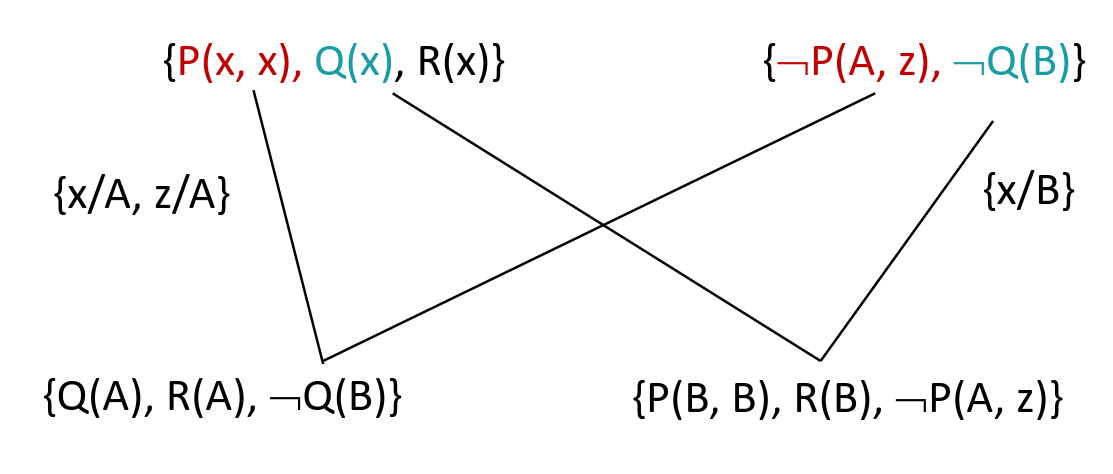
\includegraphics[scale=0.3]{fol_solution_graph.png}
	\end{center}
\end{example}

\begin{definition}[Fattori]
	Se un sottoinsieme dei letterali di una stessa clausola può essere unificato, allora la clausola ottenuta dopo tale unificazione si dice \textbf{fattore} delle clausole.
\end{definition}

\begin{observation}[Problema dei fattori]
	Ad esempio nel seguente caso le seguenti clausole dovrebbero produrre la clausola vuota, ma invece no.
	\begin{center}
		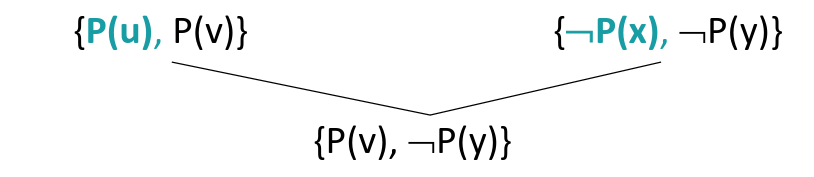
\includegraphics[scale=0.2]{fol_factors_problem.png}
	\end{center}
	È quindi necessario applicare il metodo di risoluzione ai fattori delle clausole.
	\begin{center}
		\includegraphics[scale=0.2]{fol_factors_problem_2.png}
	\end{center}
\end{observation}

La deduzione per risoluzione è \textbf{corretta} ma \textbf{non completa}. Per ottenere la completezza si può risolvere per \textbf{confutazione}.
\begin{example}
	Partiamo dalla seguente KB:
	\begin{align*}
		&\{P(A, J)\}\\
		& \{M(B, J)\}\\
		&\{\neg P(x,y), G(x,y)\}\\
		&\{\neg M(v,w), G(v,w)\}\\
		& \{\neg G(A, J)\}
	\end{align*}\\
	In questo caso il grafo è il seguente:
	\begin{center}
		\includegraphics[scale=0.3]{fol_example_refutazione.png}
	\end{center}
\end{example}

\subsection{Programmazione logica}
\subsubsection{Clausola di Horn}
Una clausola di Horn è una \textbf{disgiunzione di letterali} che contiene al massimo un letterale positivo. È un modo potente ed efficiente per rappresentare conoscenze in logica del prim'ordine. È efficace in particolare per rappresentare regole e fatti in un sistema basato su regole.
\begin{equation}
	\{Q, \neg P_1, \ldots, \neg P_k\}\quad\quad k\geq 0
\end{equation} 
Possiamo quindi scrivere la knowledge base a regole come:
\begin{align*}
	P_1 \land \ldots \land P_k \Rightarrow Q \quad \text{(regola)}&& k>0 \\
	Q \quad\text{(fatto)}&& k=0
\end{align*}
Se la knowledge base contiene solo \textit{clausole Horn} definite, i meccanismi inferenziali sono più semplici (lineari per il caso proposizionale) senza dover rinunciare alla completezza.
\subsubsection{Inferenza}
I metodi usati nei sistemi basati su regole sono di due tipi:
\begin{itemize}
	\item Inferenza in \textbf{avanti}: si inizia con le \textit{premesse} e si procede verso le conclusioni partendo da un insieme di fatti noti e applicando le regole per dedurre nuove informazioni. Si continua fino a quando non si raggiunge un obiettivo o non si possono fare più inferenze
	\item Inferenza all'\textbf{indietro}: si inizia dalle \textit{conclusioni} e si lavora a ritroso per trovare le premesse che supportano la conclusione. Si verifica passo per passo se l'obiettivo corrente può essere dedotto dalle regole e se necessario si cerca all'indietro per dedurre o dimostrare i fatti richiesti dalle premesse.
\end{itemize}

\subsubsection{Programmazione}
I programmi logici sono KB costituiti di clausole Horn definite espressi come fatti e regole:
\begin{itemize}
	\item \textbf{Fatto}: un fatto è rappresentato da una singola clausola di Horn senza premesse
	\item \textbf{Regola}: sono implicazioni logiche che descrivono i come i fatti sono in relazione tra loro
\end{itemize}

\begin{note}[Convenzioni programmazione logica]
	Nella programmazione logica le \textbf{variabili} sono indicate con le lettere maiuscole e le \textbf{costanti} con quelle minuscole.
\end{note}
L'interpretazione può seguire due filosofie:
\begin{itemize}
	\item \textbf{Dichiarativa}: data la regola
	\begin{equation*}
		A :- B_1, \ldots, B_n 
	\end{equation*}
	$A$ è vero se sono veri $B_1, \ldots, B_n$ in accordo al significato logico dell'implicazione.
	\item \textbf{Procedurale}: sempre nel caso visto nel punto precedente, si considera la testa $A$ come una chiamata di procedura e il corpo come una serie di procedure da eseguire in sequenza
\end{itemize}

\begin{example}
	\label{example:pl}
	Ad esempio definiamo le seguenti regole, fatti e goal:
	\begin{align*}
		&genitore(X, Y) :- padre(X,Y).\\
		&genitore(X, Y) :- madre(X,Y).\\
		&antenato(X, Y) :- genitore(X,Y).\\
		&antenato(X, Y) :- genitore(X,Y), antenato(Z, Y).\\
		& padre(gio, mark).\\
		& padre(gio, luc).\\
		& madre(lia, gio).\\
		&:- antenato(lia, mark:)
	\end{align*}
\end{example}

\subsubsection{Risoluzione SLD}
La risoluzione di tipo \textbf{Selection Linear Definite-Clauses} è una strategia \textbf{ordinata} e \textbf{completa} per le clausole di Horn. A partire da un programma $P$ e un goal $G$ si costruisce l'albero di risoluzione, definito come:
\begin{itemize}
	\item Ogni \textbf{nodo} dell'albero corrisponde ad un goal
	\item La \textbf{radice} è $:- G_1, \ldots, G_k$, il goal di partenza
	\item Data la radice come nodo dell'albero, questo ha tanti \textbf{discendenti} quanti sono i fatti e le regole in $P$ la cui testa è unificabile con $G_1$
	\item I nodi che sono clausole vuote sono \textbf{successi}
	\item I nodi che non hanno successori sono \textbf{fallimenti}
\end{itemize}

\begin{example}
	Dato l'esempio \ref{example:pl}, il grafo di risoluzione è:
	\begin{center}
		\includegraphics[scale=0.3]{pol_sdl.png}
	\end{center}
\end{example}

Questa strategia è \textbf{completa} per clausole di Horn definite.
	% !TeX spellcheck = it_IT
\newpage
\section{Machine learning}
\subsection{Introduzione}
L'\textbf{apprendimento} è un principio universale per esseri viventi, per la società ma anche per le macchine. È permette di fornire l'\textbf{intelligenza} a sistemi. È un campo complesso ed in continua crescita per creare:
\begin{itemize}
	\item Computer che possano \textbf{imparare}
	\item Nuovi \textbf{strumenti} potenti ed adattivi con basi rigorose nell'informatica
\end{itemize}
Permettere alle macchine di imparare ci serve perché la quantità di dati sta aumentando esponenzialmente ed è molto difficile istruire una macchina solamente tramite istruzioni imperative.\\
Tra gli obiettivi ci sono:
\begin{itemize}
	\item Costruire \textbf{sistemi adattivi intelligenti} (e.g. robot, motori di ricerca)
	\item Creare \textbf{strumenti statistici} per analizzare i dati (data science)
	\item Affrontare \textbf{nuovi problemi} fin'ora troppo complessi (e.g. ambito medico)
\end{itemize}
\begin{example}[Email spam classification]
	\label{example:email_spam}
	Identificare tramite istruzioni rigorose quali mail sono o non sono spam è molto difficile, considerando anche che può variare da persona a persona. Il machine learning in questo caso permette di costruire una \textit{classificazione} basata su degli \textit{esempi} che si possa \textit{adattare} ai vari casi.
\end{example}
\begin{example}[Face recognition]
	Nel 2014 è stata sviluppata una rete neurale che permetteva, partendo dall'apprendimento di circa 4 milioni di immagini, di riconoscere le facce umane già viste, con una percentuale di successo del $97.25\%$ (quella umana è del $97.53$).
\end{example}
\begin{example}[Go]
	Il gioco del Go, in quanto molto complesso (anche più degli scacchi), si è adattato molto bene al machine learning, che con il tempo è riuscito a battere gli umani e a diventare sempre più esperto.
\end{example}
\begin{example}[Traduzione]
	Un'altra applicazione molto famosa sono i sistemi di traduzione automatica, come Google Translate dal 2016 o DeepL dal 2017.
\end{example}
\begin{example}[Medicina]
	Il machine learning in ambito medico può aiutare in diversi aspetti: dalla diagnosi alla terapia, alle medicine personalizzate, al monitoraggio della salute e persino alla progettazione delle medicine stesse.\\
	Uno degli esempi più famosi è quello della rete neurale che permette di riconoscere il cancro alla pelle con l'accuratezza di un dermatologo certificato.
\end{example}
\begin{example}[Musica]
	Anche nell'arte, in particolare della musica, ci sono diversi esempi di Machine Learning, come AIVA, una rete neurale che è partita dalla composizione di un brano per pianoforte ed è arrivata ad orchestre e colonne sonore per videogiochi.
\end{example}
\begin{note}[Premio Turing]
	Il premio Turing del 2018 è stato vinto da tre professori, il Dr. Hinton, il Dr. LeCun e il dottor Bengio, per il loro lavoro innovativo che ha reso le reti neurali profonde un componente fondamentale per l'informatica moderna.
\end{note}

\subsubsection{Quando?}
Il machine learning deve essere utilizzato quando può essere \textbf{utile} (\textbf{opportunity}):
\begin{itemize}
	\item Per problemi di cui c'è poca o nessuna teoria
	\item In presenza di dati incerti, distorti o non completi
	\item In ambienti dinamici che non possono essere previsti in anticipo
\end{itemize}
e con criterio in base a ciò di cui ha bisogno (\textbf{awareness}):
\begin{itemize}
	\item Una fonte di apprendimento
	\item Si deve accettare che i risultati avranno una certa tolleranza
\end{itemize}

\begin{note}
	Il machine learning non è una metodologia approssimata ma bensì un metodo rigoroso per trovare una funzione approssimata che gestisca il problema complesso. Viene quindi definito \textbf{soft computing}, ovvero aperto a nuove possibilità (e.g. la biologia).
\end{note}

\subsection{Sistema predittivo}
Un sistema si compone dai \textbf{dati}, ovvero le osservazioni del mondo reale, da un \textbf{modello}, che può migliorare tramite apprendimento ed è quindi composto anche da \textit{task}, \textit{algoritmo di apprendimento} e metodo di \textit{validazione}, e da una \textbf{previsione}. 
\begin{center}
	\includegraphics[scale=0.4]{predictive_system.png}
\end{center}

Il machine learning consiste nel ricostruire una \textbf{funzione} a partire dai dati.
\begin{example}[Riconoscimento della scrittura]
	Partiamo dai dati in \textbf{ingresso}: una raccolta di immagini di scrittura a mano di cifre sotto forma di array e matrici. Vogliamo costruire un modello che, ricevuta in input un'immagine di scrittura a mano, ne predica le cifre.
	
	\begin{center}
		\includegraphics[scale=0.2]{hand_writing_recognition.png}
	\end{center}
	Il problema ha quindi una soluzione difficile da formalizzare (presenza di rumore e ambiguità nei dati) ma è facile ottenere dei dati da cui far apprendere il modello.\\
\end{example}

L'apprendimento può essere di due tipi:
\begin{itemize}
	\item \textbf{Supervisionato}: a partire da una serie di dati \textbf{supervisionati} (sappiamo che etichetta hanno), si crea una funzione che si possa applicare ad altri casi
	\item \textbf{Non supervisionato}: a partire da una serie di dati non etichettati cerchiamo \textbf{raggruppamenti naturali} come:
	\begin{itemize}
		\item Clustering
		\item Modellazione della densità dei dati
		\item Preprocessing, visualizzazione, riduzione dimensionale
	\end{itemize}
\end{itemize}

\subsubsection{Apprendimento supervisionato}
\begin{definition}[Task]
	Dato un insieme di \textbf{esempi} etichettati del tipo
	\begin{equation*}
		<input,output>=(\textbf{x},d)
	\end{equation*}
	per una \textbf{funzione} sconosciuta $f$, di cui conosciamo il valore solo per i punti in ingresso (\textbf{target value} $d$).\\
	Dobbiamo trovare una buona \textit{approssimazione} a $f$, ovvero un \textbf{ipotesi} $h$ che può essere usata per fare previsioni su dati mai visti $x'$.\\
	Il \textbf{target} può essere:
	\begin{itemize}
		\item \textbf{Categorico} per i problemi di \textbf{classificazione}: $f(\textbf{x})$ restituisce la presunta corretta classe tra $\{1,2,\ldots, k\}$
		\item \textbf{Numerico} per i problemi di \textbf{regressione}, dove $f(\textbf{x})$ restituisce valori continui
	\end{itemize}
\end{definition}

\begin{example}
	Alcuni esempi di funzioni:
	\begin{itemize}
		\item Riconoscimento di scrittura
		\begin{itemize}
			\item $\textbf{x}$: dati dalle immagini dei caratteri
			\item $f(\textbf{x})$: lettere dell'alfabeto
		\end{itemize}
		\item Diagnosi di malattie da cartella clinica
		\begin{itemize}
			\item $\textbf{x}$: dati sul paziente (sintomi, analisi di laboratorio)
			\item $f(\textbf{x})$: malattia o terapia consigliata
			\item Training set: cartella clinica del paziente
		\end{itemize}
		\item Riconoscimento facciale
		\begin{itemize}
			\item $\textbf{x}$: immagine della faccia della persona
			\item $f(\textbf{x})$: nome della persona
		\end{itemize}
		\item Riconoscimento dello spam
		\begin{itemize}
			\item $\textbf{x}$: email
			\item $f(\textbf{x})$: spam o non spam
		\end{itemize}
	\end{itemize}
\end{example}

\begin{definition}[Modello]
	Un modello ha come obiettivo quello di descrivere le relazioni tra i dati sulla base di un task. Definisce la classe della funzione che la macchina può implementare, ovvero lo \textbf{spazio delle ipotesi} (e.g. $h(\textbf{x}, \textbf{w})$ dove $w$ sono parametri astratti).
\end{definition}
\begin{definition}[Esempi di training]
	Un esempio della forma
	\begin{equation*}
		(\textbf{x}, f(\textbf{x})+noise)
	\end{equation*}
	dove $\textbf{x}$ è di solito un vettore di caratteristiche e $d=f(\textbf{x})+noise$ è il \textbf{target value}.
\end{definition}
\begin{definition}[Funzione obiettivo]
	La vera funzione $f$.
\end{definition}
\begin{definition}[Ipotesi]
	Una proposta di funzione $h$ che si crede essere simile a $f$. Un'espressione in un determinato \textbf{linguaggio} (e.g. logico, numerico o probabilistico) che descrive la relazione tra i dati.
\end{definition}
\begin{definition}[Spazio delle ipotesi]
	L'insieme di tutte le ipotesi che possono in teoria essere date in output dall'algoritmo.
\end{definition}

\noindent Alcuni modelli sono:
\begin{itemize}
	\item Modelli \textbf{lineari}, dove ogni rappresentazione di $h$ definisce uno spazio continuo di ipotesi. Ogni assegnamento di \textbf{$w$} è un'ipotesi differente. Ad esempio
	\begin{equation*}
		h_w(x)=w_1x+w_0 \quad h_w(x) = 0.232x + 246
	\end{equation*}
	\item \textbf{Regole simboliche}: lo spazio delle ipotesi è composto da rappresentazioni discrete. Si possono applicare diverse regole, ad esempio:
	\begin{lstlisting}[language=Python]
		if (x_1=0) and (x_2=1) then h(x)=1
		else h(x)=0
	\end{lstlisting}
	\item Modelli \textbf{probabilistici}: si fa una stima di $p(\textbf{x},y)$
	\item Modelli basati su \textbf{istanze}: predicono il valore medio $y$ dei vicini più prossimi (memory based)
\end{itemize}

\begin{definition}[Algoritmo di apprendimento]
	È un algoritmo che si basa sui dati, sulle task e sul modello ed impara con una ricerca euristica attraverso le ipotesi nello spazio $H$ delle migliori ipotesi (di solito cercando $h$ con l'errore minimo che si approssimi meglio alla funzione obiettivo).
	\begin{center}
		\includegraphics[scale=0.2]{learning_alg_search.png}
	\end{center}
\end{definition}

\begin{note}
	L'insieme $H$ potrebbe non coincidere con tutte le possibili funzioni e la ricerca quindi non può essere esaustiva: deve fare determinate assunzioni.
\end{note}

\begin{definition}[Funzione buona]
	Definiamo una funzione trovata come buona se è \textbf{generale}, ovvero in base a quanto è accurata nel predire i valori per nuovi dati. Ci sono quindi due fasi:
	\begin{itemize}
		\item \textbf{Learning}: il modello viene costruito da dati noti
		\item \textbf{Test}: il modello viene applicato a nuovi esempi e vengono valutate le capacità predittive in maniera \textbf{generale}
	\end{itemize}
\end{definition}
\begin{note}[Performance]
	Nel Machine Learning la performance indica l'accuratezza del modello nel predire un risultato, stimata dall'errore computo nella fase di test.
\end{note}

\subsection{Concept learning}
Il concept learning si tratta di inferire una \textbf{funzione booleana} a partire da esempi positivi o negativi.
\begin{definition}[Esempio]
	Definiamo come esempio la seguente coppia:
	\begin{equation*}
		<x,c(x)> \in D
	\end{equation*}
\end{definition}
\begin{definition}[Soddisfa]
	Una funzione $h:X\to\{0,1\}$ soddisfa $x$ se
	\begin{equation*}
		h(x)=1
	\end{equation*}
\end{definition}
\begin{definition}[Consistenza]
	Un'ipotesi $h$ è consistente con:
	\begin{itemize}
		\item un \textbf{esempio} $<x,c(x)> \quad x \in X$ se $h(x) = c(x)$
		\item un \textbf{insieme di esempi} $D$ se $\forall <x,c(x)> \in D \Longrightarrow h(x) = c(x)$
	\end{itemize}
\end{definition}
\begin{definition}[Problema mal posto]
	Un problema si dice mal posto quando viola:
	\begin{itemize}
		\item L'\textbf{esistenza}
		\item L'\textbf{unicità}
		\item La \textbf{stabilità}
	\end{itemize}
	della soluzione.
\end{definition}
\begin{definition}[Spazio delle ipotesi]
	Dati $n$ input binari, lo spazio delle ipotesi è:
	\begin{equation}
		\lvert H \rvert = 2^{\#-instances}=2^{2^n}
	\end{equation}
\end{definition}
\begin{example}[Funzioni booleane]
	Dati dei valori booleani in input di cui sappiamo l'output, dobbiamo determinare la funzione booleana.
	\begin{table}[!h]
		\centering
		\includegraphics[scale=0.3]{boolean_function.png}
		\begin{tabular}{cccc|c}
			$x_1$ & $x_2$ & $x_3$ & $x_4$ & y \\
			\hline
			0 & 0 & 1 & 0 & 0 \\
			0 & 1 & 0 & 0 & 0 \\
			0 & 0 & 1 & 1 & 1 \\
			1 & 0 & 0  &1 & 1 \\
			0 & 1 & 1 & 0 & 0 \\
			1 & 1 & 0 & 0 & 0 \\
			0 & 1 & 0 & 1 & 0 \\
			\hline
		\end{tabular}
	\end{table}
	\\Questo è una problema \textbf{mal posto} in quanto ci sono più funzioni che potrebbero dare questo risultato (\textbf{unicità}).
	Dati quattro input binari, abbiamo $2^{2^4}= 65536 $ possibili funzioni che dobbiamo esplorare interamente per trovare quella corretta.\\
	È necessario lavorare con uno spazio ristretto di ipotesi $H$.
\end{example}
\begin{definition}[Lookup table]
	Un possibile modello di ML è quello di \textit{Lookup Table}, dove l'algoritmo sa a memoria le risposte che gli sono state date in ingresso e sa rispondere solo se gli viene chiesta una di quelle.
\end{definition}
\subsubsection{Conjective Rules}
Tramite il costrutto \textbf{AND} possiamo ridurre lo spazio delle ipotesi. Considerando dei letterali $l_i$ come pezzo di una stringa di lunghezza $n$, abbiamo:
\begin{itemize}
	\item Letterali \textbf{positivi} (e.g. $h_1=l_2$, $h2=l_1 \land l_2$, $h_3=true$): $\lvert H \rvert = 2^n$
	\item Letterali anche \textbf{negativi} (e.g. $not(l_i)$): $\lvert H \rvert = 3^n + 1$
\end{itemize}

\begin{example}[Enjoy sport]
	\label{example:enjoy_sport}
	Supponiamo di avere determinati \textbf{attributi} relativi al tempo meteorologico e in corrispondenza se una persona vuole o meno fare sport.\\
	Abbiamo quindi $X$ \textbf{istanze}, una \textbf{funzione obiettivo} ($c:EnjoySport \: X \to \{0,1\}$) e un \textbf{training set} $l$ composto da coppie di tipo $<x_n,c(x_l)$
	\begin{table}[!h]
		\centering
		\begin{tabular}{|ccccccc|}
			\hline
			Sky & Temp & Humid & Wind & Water & Forecast & Enjoy \\
			\hline
			Sunny & Warm & Normal & Strong & Warm & Same & Yes \\
			Sunny & Warm & High & Strong & Warm & Same & Yes \\
			Rainy & Cold & High & Strong & Warm & Change & No \\
			Sunny & Warm & High & Strong & Cool & Change & Yes \\
			\hline
		\end{tabular}
	\end{table}
	\\Rappresentiamo ogni \textbf{ipotesi} come insieme di vincoli sugli attributi scelto tra:
	\begin{itemize}
		\item Un valore specifico, e.g. $Water=Warm$
		\item Un valore che non ci interessa, e.g. $Water=?$
		\item Nessun valore permesso (ipotesi nulla), e.g. $Water=\emptyset$
	\end{itemize}
	Una possibile \textit{ipotesi} (per cui quindi una persona va a fare sport) è la seguente:
	\begin{equation*}
		Sky=Sunny \land Wind=Strong \land Forecast=Same
	\end{equation*}
	L'ipotesi più specifica avrà tutti valori \textit{nulli} mentre quella più generale avrà tutti valori che non ci interessano.\\
	L'\textbf{obiettivo} è quello di trovare un'ipotesi $h$ tale che $h(x)=c(x) \forall x \in X$.
	\begin{note}
		Per ora assumiamo che ogni ipotesi che approssimi la funzione obiettivo correttamente sui training examples, approssimerà anche la funzione sugli esempi non osservati. In generale uno dei problemi fondamentali del ML è la differenza tra analisi teorica ed empirica.
	\end{note}
	Per questo esempio abbiamo
	\begin{equation*}
		3 \cdot 2 \cdot 2 \cdot 2 \cdot 2 \cdot 2 = 96
	\end{equation*}
	istanze distinte e $2^{96}$ \textbf{funzioni possibili}. Possiamo semplificare prendendo le ipotesi \textit{sintatticamente} distinte, ovvero $5\cdot 4 \cdot 4 \cdot4 \cdot 4 \cdot 4 = 5120$, oppure quelle \textit{semanticamente} distinte, ovvero $1+4\cdot3\cdot3\cdot3\cdot3\cdot3 = 973$.
\end{example}

\begin{definition}[Più generale]
	Siano $h_j$ e $h_k$ funzioni booleane definite su $X$. $h_j$ è più generale o uguale di $h_k$ se e solo se:
	\begin{equation}
		\forall x \in X : [(h_k(x) = 1) \to (h_j(x)=1)]
	\end{equation}
\end{definition}
In questo modo possiamo imporre un ordinamento sulle \textit{ipotesi}, del tipo $l_i : l_1 \geq (l_1 \land l_2)$, e strutturarne lo spazio dalle più specifiche alle più generali.
\begin{center}
	\includegraphics[scale=0.3]{hyp_ordin.png}
\end{center}
\subsubsection{Find-S}
Un algoritmo per cercare una soluzione prevede di ordinare le ipotesi e cercare la più specifica senza bisogno di enumerarle tutte:
\begin{enumerate}
	\item Inizializza $h$ all'ipotesi più specifica in $H$
	\item Per ogni training istance $x$ \textbf{positiva}:
	\begin{lstlisting}
		for each attribute a[i] in h
			if a[i] in h is statisfied by x
				do nothing
			else
				replace a[i] in h by the next more general costraint satisfied by x
	\end{lstlisting}
	\item Restituisci l'ipotesi $h$
\end{enumerate}
\begin{example}
	Partendo dall'esempio \ref{example:enjoy_sport}, facciamo i seguenti passi:
	\begin{enumerate}
		\item $h_0=<\emptyset,\emptyset,\emptyset,\emptyset,\emptyset>$ è la prima ipotesi
		\item Non soddisfa $x_1$. Mettiamo tutti gli attributi in modo che soddisfino al minimo $x_1$. Otteniamo $h_1=<Sunny,Warm,Normal,Strong,Warm,Same>$
		\item $h_1$ non soddisfa $x_2$. Per soddisfarla generalizziamo ulteriormente l'attributo $Humid$, ottenendo $h_2=<Sunny,Warm,?,Strong,Warm,Same>$
		\item $x_3$ è negativa, quindi non la consideriamo
		\item $h_2$ non soddisfa $x_4$. Generalizziamo gli attributi $Water$ e $Forecast$ e otteniamo \\$h_3=<Sunny,Warm,?,Strong,?,?>$
	\end{enumerate}
\end{example}
Questo algoritmo permette di trovare l'ipotesi più specifica che sia consistente con il training example (anche per gli esempi negativi).\\
Un problema è che non c'è \textbf{tolleranza al rumore}, ovvero che non valutando gli esempi negativi non sappiamo se ci sono delle contraddizioni. Inoltre trova solo una soluzione.

\subsubsection{List-Then-Eliminate}
L'idea è di ottenere una descrizione dell'insieme di tutte le ipotesi che siano consistenti con il training example.
\begin{definition}[Version space]
	Il version space $VS_{H,D}$ rispetto allo spazio delle ipotesi $H$ e al training set $D$ è il sottoinsieme delle ipotesi che sono consistenti con tutti i casi del training examples
	\begin{equation}
		VS_{H,D}=\{h \in H \vert Consistent(h,D)\}
	\end{equation}
\end{definition}
L'algoritmo prevede i seguenti passi:
\begin{enumerate}
	\item Faccio una lista di tutte le ipotesi (VersionSpace) $H$
	\item Per ogni training example $<x,c(x)$ rimuovo ogni ipotesi del VS che è inconsistente con quell'esempio
	\item Restituisco il VS
\end{enumerate}
È un algoritmo irrealistico in quanto dovremmo enumerare tutte le ipotesi.
\subsubsection{Candidate Elimination}
Per evitare di enumerare tutte le ipotesi, possiamo definire il Version Space con dei limiti generali e specifici.
\begin{definition}[General boundary]
	Il limite generale $G$ di un version space $VS_{H,D}$ è l'insieme delle ipotesi più generali in $H$ consistenti con $D$.
\end{definition}
\begin{definition}[Specific boundary]
	Il limite specifico $G$ di un version space $VS_{H,D}$ è l'insieme delle ipotesi più specifiche in $H$ consistenti con $D$.
\end{definition}
\begin{theorem}
	Ogni membro del version space si trova tra il \textbf{general} e lo \textbf{specific} boundary.
	\begin{equation}
		VS_{H,D} = \{h \in H \vert (\exists s \in S) (\exists g \in G) (g\geq h \geq s)\}
	\end{equation}
\end{theorem}
L'algoritmo prevede, per ogni training example $d$, dato $G$ l'insieme delle ipotesi più generali e $S$ quello delle ipotesi più specifiche:
\begin{itemize}
	\item Se $d$ è \textbf{positivo}:
	\begin{enumerate}
		\item Rimuovo da $G$ ogni ipotesi che non sia consistente con $d$
		\item Per ogni ipotesi $s$ che non è consistente con $d$:
		\begin{itemize}
			\item Rimuovo $s$ da $S$
			\item Aggiungo a $S$ tuute le ipotesi $h$ sufficientemente generalizzate in modo che $h$ sia consistente con $d$ e che alcuni elementi di $G$ siano più generali di $h$
			\item Rimuovo da $S$ ogni ipotesi che sia più generale di un'altra ipotesi in $S$
		\end{itemize}
	\end{enumerate}
	\item Se $d$ è \textbf{negativo}:
	\begin{enumerate}
		\item Rimuovo da $S$ ogni ipotesi che non sia consistente con $d$
		\item Per ogni ipotesi $g$ che non è consistente con $d$:
		\begin{itemize}
			\item Rimuovo $g$ da $G$
			\item Aggiungo a $G$ tuute le ipotesi $h$ sufficientemente specializzate in modo che $h$ sia consistente con $d$ e che alcuni elementi di $S$ siano più specializzati di $h$
			\item Rimuovo da $G$ ogni ipotesi che sia meno generale di un'altra ipotesi in $G$
		\end{itemize}
	\end{enumerate}
\end{itemize}
Per \textbf{classificare} i nuovi dati, testiamo la loro consistenza con il version space e vediamo con quante delle ipotesi dà risultato positivo o negativo.

\subsubsection{Bias induttivo}
Il version space non può rappresentare le disgiunzioni (e.g. soleggiato O nuvoloso). Per rimuovere il bias possiamo scegliere uno spazio delle ipotesi $H$ che contenga ogni singolo concetto, ovvero tutti i possibili sottoinsiemi di $X$. Se abbiamo ad esempio $\lvert X \rvert=96$ allora ci sono $\lvert P(X)\rvert = 2^{96}$ concetti distinti. \\
Questa generalizzazione, oltre ad aumentare il tempo necessario per la ricerca, impedisce al modello di classificare nuovi esempi che non siano del training set.
\begin{definition}[Unbiased learner]
	Un unbiased learner non è in grado di generalizzare, in quanto ogni istanza non osservata sarà classificata positivamente da metà delle ipotesi e negativamente dall'altra metà. Ci ritroveremmo quindi con una \textbf{Lookup Table}.
\end{definition}
\noindent Le restrizioni che si fanno sono quindi \textbf{necessarie} per potere fare una generalizzazione. È importante quindi caratterizzare il bias utilizzato e capire qual'è il migliore da scegliere.

\begin{definition}[Inductive bias]
	Il bias induttivo di una algoritmo $L$ è ogni minimo insieme di assunzioni $B$ tali che per ogni concetto obiettivo $c$ e il corrispondente training data $D_c$
	\begin{equation}
		(\forall x_i \in X)[B \land D_c \land x_i] \vdash L(x_i, D_c)
	\end{equation}
	In pratica posso trasformarlo in un sistema \textbf{deduttivo}.
\end{definition}
Negli algoritmi visti fin'ora abbiamo trovato i seguenti bias:
\begin{itemize}
	\item \textbf{Lookup table}: nessun bias
	\item \textbf{Find-S}: lo spazio delle ipotesi contiene il target concept e tutte le istanza sono negative a meno che gli esempi positivi non ci dicano il contrario
	\item \textbf{Candidate Elimination}: lo spazio delle ipotesi contiene il target concept
\end{itemize}
	% !TeX spellcheck = it_IT
\newpage
\section{Concept learning}
Il concept learning si tratta di inferire una \textbf{funzione booleana} a partire da esempi positivi o negativi.
\begin{definition}[Esempio]
	Definiamo come esempio la seguente coppia:
	\begin{equation*}
		<x,c(x)> \in D
	\end{equation*}
\end{definition}
\begin{definition}[Soddisfa]
	Una funzione $h:X\to\{0,1\}$ soddisfa $x$ se
	\begin{equation*}
		h(x)=1
	\end{equation*}
\end{definition}
\begin{definition}[Consistenza]
	Un'ipotesi $h$ è consistente con:
	\begin{itemize}
		\item un \textbf{esempio} $<x,c(x)> \quad x \in X$ se $h(x) = c(x)$
		\item un \textbf{insieme di esempi} $D$ se $\forall <x,c(x)> \in D \Longrightarrow h(x) = c(x)$
	\end{itemize}
\end{definition}
\begin{definition}[Problema mal posto]
	Un problema si dice mal posto quando viola:
	\begin{itemize}
		\item L'\textbf{esistenza}
		\item L'\textbf{unicità}
		\item La \textbf{stabilità}
	\end{itemize}
	della soluzione.
\end{definition}
\begin{definition}[Spazio delle ipotesi]
	Dati $n$ input binari, lo spazio delle ipotesi è:
	\begin{equation}
		\lvert H \rvert = 2^{\#-instances}=2^{2^n}
	\end{equation}
\end{definition}
\begin{example}[Funzioni booleane]
	Dati dei valori booleani in input di cui sappiamo l'output, dobbiamo determinare la funzione booleana.
	\begin{table}[!h]
		\centering
		\includegraphics[scale=0.3]{boolean_function.png}
		\begin{tabular}{cccc|c}
			$x_1$ & $x_2$ & $x_3$ & $x_4$ & y \\
			\hline
			0 & 0 & 1 & 0 & 0 \\
			0 & 1 & 0 & 0 & 0 \\
			0 & 0 & 1 & 1 & 1 \\
			1 & 0 & 0  &1 & 1 \\
			0 & 1 & 1 & 0 & 0 \\
			1 & 1 & 0 & 0 & 0 \\
			0 & 1 & 0 & 1 & 0 \\
			\hline
		\end{tabular}
	\end{table}
	\\Questo è una problema \textbf{mal posto} in quanto ci sono più funzioni che potrebbero dare questo risultato (\textbf{unicità}).
	Dati quattro input binari, abbiamo $2^{2^4}= 65536 $ possibili funzioni che dobbiamo esplorare interamente per trovare quella corretta.\\
	È necessario lavorare con uno spazio ristretto di ipotesi $H$.
\end{example}
\begin{definition}[Lookup table]
	Un possibile modello di ML è quello di \textit{Lookup Table}, dove l'algoritmo sa a memoria le risposte che gli sono state date in ingresso e sa rispondere solo se gli viene chiesta una di quelle.
\end{definition}
\subsection{Conjective Rules}
Tramite il costrutto \textbf{AND} possiamo ridurre lo spazio delle ipotesi. Considerando dei letterali $l_i$ come pezzo di una stringa di lunghezza $n$, abbiamo:
\begin{itemize}
	\item Letterali \textbf{positivi} (e.g. $h_1=l_2$, $h2=l_1 \land l_2$, $h_3=true$): $\lvert H \rvert = 2^n$
	\item Letterali anche \textbf{negativi} (e.g. $not(l_i)$): $\lvert H \rvert = 3^n + 1$
\end{itemize}

\begin{example}[Enjoy sport]
	\label{example:enjoy_sport}
	Supponiamo di avere determinati \textbf{attributi} relativi al tempo meteorologico e in corrispondenza se una persona vuole o meno fare sport.\\
	Abbiamo quindi $X$ \textbf{istanze}, una \textbf{funzione obiettivo} ($c:EnjoySport \: X \to \{0,1\}$) e un \textbf{training set} $l$ composto da coppie di tipo $<x_n,c(x_l)$
	\begin{table}[!h]
		\centering
		\begin{tabular}{|ccccccc|}
			\hline
			Sky & Temp & Humid & Wind & Water & Forecast & Enjoy \\
			\hline
			Sunny & Warm & Normal & Strong & Warm & Same & Yes \\
			Sunny & Warm & High & Strong & Warm & Same & Yes \\
			Rainy & Cold & High & Strong & Warm & Change & No \\
			Sunny & Warm & High & Strong & Cool & Change & Yes \\
			\hline
		\end{tabular}
	\end{table}
	\\Rappresentiamo ogni \textbf{ipotesi} come insieme di vincoli sugli attributi scelto tra:
	\begin{itemize}
		\item Un valore specifico, e.g. $Water=Warm$
		\item Un valore che non ci interessa, e.g. $Water=?$
		\item Nessun valore permesso (ipotesi nulla), e.g. $Water=\emptyset$
	\end{itemize}
	Una possibile \textit{ipotesi} (per cui quindi una persona va a fare sport) è la seguente:
	\begin{equation*}
		Sky=Sunny \land Wind=Strong \land Forecast=Same
	\end{equation*}
	L'ipotesi più specifica avrà tutti valori \textit{nulli} mentre quella più generale avrà tutti valori che non ci interessano.\\
	L'\textbf{obiettivo} è quello di trovare un'ipotesi $h$ tale che $h(x)=c(x) \forall x \in X$.
	\begin{note}
		Per ora assumiamo che ogni ipotesi che approssimi la funzione obiettivo correttamente sui training examples, approssimerà anche la funzione sugli esempi non osservati. In generale uno dei problemi fondamentali del ML è la differenza tra analisi teorica ed empirica.
	\end{note}
	Per questo esempio abbiamo
	\begin{equation*}
		3 \cdot 2 \cdot 2 \cdot 2 \cdot 2 \cdot 2 = 96
	\end{equation*}
	istanze distinte e $2^{96}$ \textbf{funzioni possibili}. Possiamo semplificare prendendo le ipotesi \textit{sintatticamente} distinte, ovvero $5\cdot 4 \cdot 4 \cdot4 \cdot 4 \cdot 4 = 5120$, oppure quelle \textit{semanticamente} distinte, ovvero $1+4\cdot3\cdot3\cdot3\cdot3\cdot3 = 973$.
\end{example}

\begin{definition}[Più generale]
	Siano $h_j$ e $h_k$ funzioni booleane definite su $X$. $h_j$ è più generale o uguale di $h_k$ se e solo se:
	\begin{equation}
		\forall x \in X : [(h_k(x) = 1) \to (h_j(x)=1)]
	\end{equation}
\end{definition}
In questo modo possiamo imporre un ordinamento sulle \textit{ipotesi}, del tipo $l_i : l_1 \geq (l_1 \land l_2)$, e strutturarne lo spazio dalle più specifiche alle più generali.
\begin{center}
	\includegraphics[scale=0.3]{hyp_ordin.png}
\end{center}
\subsubsection{Find-S}
Un algoritmo per cercare una soluzione prevede di ordinare le ipotesi e cercare la più specifica senza bisogno di enumerarle tutte:
\begin{enumerate}
	\item Inizializza $h$ all'ipotesi più specifica in $H$
	\item Per ogni training istance $x$ \textbf{positiva}:
	\begin{lstlisting}
		for each attribute a[i] in h
		if a[i] in h is statisfied by x
		do nothing
		else
		replace a[i] in h by the next more general costraint satisfied by x
	\end{lstlisting}
	\item Restituisci l'ipotesi $h$
\end{enumerate}
\begin{example}
	Partendo dall'esempio \ref{example:enjoy_sport}, facciamo i seguenti passi:
	\begin{enumerate}
		\item $h_0=<\emptyset,\emptyset,\emptyset,\emptyset,\emptyset>$ è la prima ipotesi
		\item Non soddisfa $x_1$. Mettiamo tutti gli attributi in modo che soddisfino al minimo $x_1$. Otteniamo $h_1=<Sunny,Warm,Normal,Strong,Warm,Same>$
		\item $h_1$ non soddisfa $x_2$. Per soddisfarla generalizziamo ulteriormente l'attributo $Humid$, ottenendo $h_2=<Sunny,Warm,?,Strong,Warm,Same>$
		\item $x_3$ è negativa, quindi non la consideriamo
		\item $h_2$ non soddisfa $x_4$. Generalizziamo gli attributi $Water$ e $Forecast$ e otteniamo \\$h_3=<Sunny,Warm,?,Strong,?,?>$
	\end{enumerate}
\end{example}
Questo algoritmo permette di trovare l'ipotesi più specifica che sia consistente con il training example (anche per gli esempi negativi).\\
Un problema è che non c'è \textbf{tolleranza al rumore}, ovvero che non valutando gli esempi negativi non sappiamo se ci sono delle contraddizioni. Inoltre trova solo una soluzione.

\subsubsection{List-Then-Eliminate}
L'idea è di ottenere una descrizione dell'insieme di tutte le ipotesi che siano consistenti con il training example.
\begin{definition}[Version space]
	Il version space $VS_{H,D}$ rispetto allo spazio delle ipotesi $H$ e al training set $D$ è il sottoinsieme delle ipotesi che sono consistenti con tutti i casi del training examples
	\begin{equation}
		VS_{H,D}=\{h \in H \vert Consistent(h,D)\}
	\end{equation}
\end{definition}
L'algoritmo prevede i seguenti passi:
\begin{enumerate}
	\item Faccio una lista di tutte le ipotesi (VersionSpace) $H$
	\item Per ogni training example $<x,c(x)$ rimuovo ogni ipotesi del VS che è inconsistente con quell'esempio
	\item Restituisco il VS
\end{enumerate}
È un algoritmo irrealistico in quanto dovremmo enumerare tutte le ipotesi.
\subsubsection{Candidate Elimination}
\label{alg:cand_elim}
Per evitare di enumerare tutte le ipotesi, possiamo definire il Version Space con dei limiti generali e specifici.
\begin{definition}[General boundary]
	Il limite generale $G$ di un version space $VS_{H,D}$ è l'insieme delle ipotesi più generali in $H$ consistenti con $D$.
\end{definition}
\begin{definition}[Specific boundary]
	Il limite specifico $G$ di un version space $VS_{H,D}$ è l'insieme delle ipotesi più specifiche in $H$ consistenti con $D$.
\end{definition}
\begin{theorem}
	Ogni membro del version space si trova tra il \textbf{general} e lo \textbf{specific} boundary.
	\begin{equation}
		VS_{H,D} = \{h \in H \vert (\exists s \in S) (\exists g \in G) (g\geq h \geq s)\}
	\end{equation}
\end{theorem}
L'algoritmo prevede, per ogni training example $d$, dato $G$ l'insieme delle ipotesi più generali e $S$ quello delle ipotesi più specifiche:
\begin{itemize}
	\item Se $d$ è \textbf{positivo}:
	\begin{enumerate}
		\item Rimuovo da $G$ ogni ipotesi che non sia consistente con $d$
		\item Per ogni ipotesi $s$ che non è consistente con $d$:
		\begin{itemize}
			\item Rimuovo $s$ da $S$
			\item Aggiungo a $S$ tuute le ipotesi $h$ sufficientemente generalizzate in modo che $h$ sia consistente con $d$ e che alcuni elementi di $G$ siano più generali di $h$
			\item Rimuovo da $S$ ogni ipotesi che sia più generale di un'altra ipotesi in $S$
		\end{itemize}
	\end{enumerate}
	\item Se $d$ è \textbf{negativo}:
	\begin{enumerate}
		\item Rimuovo da $S$ ogni ipotesi che non sia consistente con $d$
		\item Per ogni ipotesi $g$ che non è consistente con $d$:
		\begin{itemize}
			\item Rimuovo $g$ da $G$
			\item Aggiungo a $G$ tuute le ipotesi $h$ sufficientemente specializzate in modo che $h$ sia consistente con $d$ e che alcuni elementi di $S$ siano più specializzati di $h$
			\item Rimuovo da $G$ ogni ipotesi che sia meno generale di un'altra ipotesi in $G$
		\end{itemize}
	\end{enumerate}
\end{itemize}
Per \textbf{classificare} i nuovi dati, testiamo la loro consistenza con il version space e vediamo con quante delle ipotesi dà risultato positivo o negativo.

\subsubsection{Bias induttivo}
Il version space non può rappresentare le disgiunzioni (e.g. soleggiato O nuvoloso). Per rimuovere il bias possiamo scegliere uno spazio delle ipotesi $H$ che contenga ogni singolo concetto, ovvero tutti i possibili sottoinsiemi di $X$. Se abbiamo ad esempio $\lvert X \rvert=96$ allora ci sono $\lvert P(X)\rvert = 2^{96}$ concetti distinti. \\
Questa generalizzazione, oltre ad aumentare il tempo necessario per la ricerca, impedisce al modello di classificare nuovi esempi che non siano del training set.
\begin{definition}[Unbiased learner]
	Un unbiased learner non è in grado di generalizzare, in quanto ogni istanza non osservata sarà classificata positivamente da metà delle ipotesi e negativamente dall'altra metà. Ci ritroveremmo quindi con una \textbf{Lookup Table}.
\end{definition}
\noindent Le restrizioni che si fanno sono quindi \textbf{necessarie} per potere fare una generalizzazione. È importante quindi caratterizzare il bias utilizzato e capire qual'è il migliore da scegliere.

\begin{definition}[Inductive bias]
	Il bias induttivo di una algoritmo $L$ è ogni minimo insieme di assunzioni $B$ tali che per ogni concetto obiettivo $c$ e il corrispondente training data $D_c$
	\begin{equation}
		(\forall x_i \in X)[B \land D_c \land x_i] \vdash L(x_i, D_c)
	\end{equation}
	In pratica posso trasformarlo in un sistema \textbf{deduttivo}.
\end{definition}
Negli algoritmi visti fin'ora abbiamo trovato i seguenti bias:
\begin{itemize}
	\item \textbf{Lookup table}: nessun bias
	\item \textbf{Find-S}: lo spazio delle ipotesi contiene il target concept e tutte le istanza sono negative a meno che gli esempi positivi non ci dicano il contrario
	\item \textbf{Candidate Elimination}: lo spazio delle ipotesi contiene il target concept (\textbf{language bias})
\end{itemize}

\subsection{Decision tree}
Introduciamo questa tecnica er risolvere la mancanza di flessibilità del concept learning.

\begin{example}[Tennis]
	\label{example:tennis}
	Poniamo di avere i seguenti dati:
	\begin{table}[H]
		\centering
		\begin{tabular}{|c|ccccc|}
			\hline
			\textbf{Day} & \textbf{Outlook} & \textbf{Temperature} & \textbf{Humidity} & \textbf{Wind} & \textbf{PlayTennis} \\
			\hline
			D1 & Sunny & Hot & High & Weak & No \\
			D2 & Sunny & Hot & High & Strong & No \\
			D3 & Overcast & Hot & High & Weak & Yes \\
			D4 & Rain & Mild & High & Weak & Yes \\
			D5 & Rain & Cool & Normal & Weak & Yes \\
			D6 & Rain & Cool & Normal & Strong & No \\
			D7 & Overcast & Cool & Normal & Strong & Yes \\
			D8 & Sunny & Mild & High & Weak & No \\
			D9 & Sunny & Cool & Normal & Weak & Yes \\
			D10 & Rain & Mild & Normal & Weak & Yes \\
			D11 & Sunny & Mild & Normal & Strong & Yes \\
			D12 & Overcast & Mild & High & Strong & Yes \\
			D13 & Overcast & Hot & Normal & Weak & Yes \\
			D14 & Rain & Mild & High & Strong & No \\
			\hline
		\end{tabular}
	\end{table}
	Un possibile \textit{albero di decisione} è il seguente:
	\begin{center}
		\includegraphics[scale=0.25]{decision_tree_tennis.png}
	\end{center}
	che può anche essere scritto come disgiunzione di congiunzioni:
	\begin{align*}
		& (Outlook=Sunny \land Humidity=Normal) \lor \\
		& (Outlook = Overcast) \lor \\
		& (Outlook=Rain \land Wind=Weak)
	\end{align*}
\end{example}

\subsubsection{ID3}
Dato un insieme di training examples, l'algoritmo fa una ricerca nello spazio degli alberi di decisione e lo costruisce \textbf{top-down} tramite una ricerca \textbf{greedy}. Il punto cruciale è la scelta dell'attributo successivo che possa dare più informazioni. Alla fine, una volta che tutti i casi sono coperti, viene ricostruito ricorsivamente l'albero.
\begin{lstlisting}
	ID3(X: training_ex, T:target_attr, Attrs: other_attr)
	Create Root node
	If all X are +, return Root with class +
	If all X are -, return Root with class -
	If Attrs is empty return Root with class most common value of T in X
	else
	A<- best attribute; decision attribute for Root <- A
	For each possible value v[i] of A:
	- add a new branch below Root, for test A = v[i]
	- X[i] <- subset of X with A = v[i]
	- If X[i] is empty then add a new leaf with class the most common value of T in X
	else add the subtree generated by ID3(X[i], T, Attrs - {A})
	return Root
\end{lstlisting}
Per selezionare il miglior attributo, utilizziamo il concetto di \textbf{entropia}.
\begin{definition}[Entropia]
	L'entropia misura l'impurità di un'insieme di esempi. Dipende dalla distribuzione della variabile casuale $p$.\\
	Dati:
	\begin{itemize}
		\item $S$ un insieme di training examples
		\item $p_+$ la proporzione di esempi positivi in $S$
		\item $p_-$ la proporzione di esempi negativi in $S$
	\end{itemize}
	la definiamo come
	\begin{equation}
		Entropy(S)=-p_+\log_2p_+ - p_-\log_2p_-
	\end{equation}
	Si noti che $0 \leq p \leq 1$ e $0 \leq Entropy \leq 1$
\end{definition}

\begin{definition}[Information gain]
	È la riduzione aspettata dell'entropia causata dal partizionamento degli esempi in base ad un determinato attributo $A$.
	\begin{equation}
		Gain(S,A) = Entropy(S) - \sum_{v \in Values(A)} \frac{\lvert S v \rvert}{\lvert S \rvert} Entropy(Sv)
	\end{equation}
	dove $Sv$ è il sottoinsieme di $S$ per cui $A$ assume valore $v$.
\end{definition}
Più è alto l'\textit{information gain} e più è efficace quel determinato attributo nel classificare i dati. Ci servono quindi degli attributi \textbf{omogenei} (ad esempio totalmente positivi o totalmente negativi). Dobbiamo quindi trovare un attributo $A$ che \textbf{massimizzi} il $Gain$, ovvero con \textbf{bassa} entropia.

\begin{example}
	Partendo dai dati dell'esempio \ref{example:tennis}, calcoliamo prima l'entropia per i vari attributi (9 positivi, 5 negativi):
	\begin{equation*}
		-\frac{9}{14} \log_2(\frac{9}{14}) - \frac{9}{14} \log_2(\frac{9}{14})=0.940
	\end{equation*}
	e poi dei singoli valori che possono assumere, per esempio guardando \textit{Humidity} e \textit{Wind}:
	\begin{itemize}
		\item \textit{Humidity} alta (3 casi positivi e 4 negativi): $-\frac{3}{7} \log_2(\frac{3}{7}) - \frac{4}{7} \log_2(\frac{4}{7})=0.985$
		\item \textit{Humidity} normale (6 casi positivi e 1 negativo): $-\frac{6}{7} \log_2(\frac{6}{7}) - \frac{1}{7} \log_2(\frac{1}{7})=0.592$
		\item \textit{Wind} debole (6 casi positivi e 2 negativi): $-\frac{6}{8} \log_2(\frac{6}{6}) - \frac{2}{8} \log_2(\frac{2}{8})=0.811$
		\item \textit{Wind} forte (3 casi positivi e 3 negativi): $-\frac{3}{6} \log_2(\frac{3}{6}) - \frac{3}{6} \log_2(\frac{3}{6})=1.00$
	\end{itemize}
	Verifichiamo poi il gain dei due attributi selezionati:
	\begin{align*}
		& Gain(S, Humidity) = 0.940 - \frac{7}{14} 0.985 - \frac{7}{14} 0.952 = 0.151 \\
		& Gain(S, Wind) = 0.940 - \frac{8}{14} 0.811 - \frac{6}{14} 1.00 = 0.048
	\end{align*}
	E vediamo che il Gain massimo lo otteniamo scegliendo il parametro Humidity (per cui avevamo trovato un valore minimo di entropia).
\end{example}

\begin{observation}
	L'information gain favorisce gli attributi con tanti possibili valori. Ad esempio nel caso \ref{example:tennis}, la Data avrebbe un gain massimo in quanto ogni giorno corrisponde ad un sottoinsieme puro diverso (quindi 0 entropia). Però non è significativo e utile per generalizzare per istanze nuove.
\end{observation}

\newpage
\noindent Per ovviare a questo problema, introduciamo il Gain Ratio.
\begin{definition}[Gain Ratio]
	Il Gain Ratio si definisce come:
	\begin{equation}
		GainRatio(S,A)=\frac{Gain(S,A)}{SplitInformation(S,A)}
	\end{equation}
	dove, date delle partizioni di $A$ su $v_i$ fino a $c$ valori,
	\begin{equation}
		SplitInformation(S,A)=-\sum_{i=1}^{c}\frac{\lvert S_i \rvert}{\lvert S\rvert} \log_2 \frac{\lvert S_i \rvert}{\lvert S \rvert}
	\end{equation}
	ovvero la misura dell'entropia di $S$ rispetto ai valori di $A$. Più sono uniformemente dispersi i dati e maggiore è il suo valore.
\end{definition}

Adesso il problema è che lo \textit{SplitInformation} può essere $0$ quando $\lvert S_i \rvert \approx \lvert S \rvert$ per un qualche valore $i$. Ovvero quando un attributo ha lo stesso valore per tutti gli esempi. Quindi prima calcoliamo il \textit{Gain} e applichiamo il \textit{GainRatio} solo ai casi che superano una certa soglia.\\
Rispetto al \hyperref[alg:cand_elim]{Candidate Elimination}, adesso:
\begin{itemize}
	\item Lo spazio delle ipotesi è \textbf{completo}
	\item La ricerca mantiene una singola ipotesi corrente
	\item Non c'è backtracking e quindi non c'è la garanzia di ottimalità
	\item Usa tutti gli esempi
	\item Può terminare prima accettando classi imperfette
\end{itemize}

In questo algoritmo il \textbf{bias induttivo} è composto da:
\begin{itemize}
	\item Preferisce alberi più corti a quelli più lunghi
	\item Preferisce alberi che mettono attributi con \textit{Gain} maggiori più vicini alla radice
\end{itemize}
ed è chiamato \textbf{search bias}. Questo è meglio del bias del \textit{Concept Learning} perché non limita la ricerca dall'inizio e permette comunque di avere uno spazio di ricerca ampio.

\begin{definition}[Rasoio di Occam]
	La spiegazione più semplice è più probabilmente la corretta. Nel caso dell'algoritmo ID3, significa di cercare di mantenere un albero più compatto.
\end{definition}

\subsubsection{Overfitting}
\begin{definition}[Overfitting]
	Consideriamo l'errore di un'ipotesi $h$ sia sui dati di training ($error_D(h)$) che su tutti i dati ($error_X(h)$). L'ipotesi $h$ overfitta i dati di training se non esiste un'ipotesi alternativa $h' \in H$ tale che:
	\begin{align*}
		& error_D(h) < error_D(h') \\
		& error_X(h')<error_X(h)
	\end{align*}
\end{definition}
\noindent Nel caso del decision tree:
\begin{center}
	\includegraphics[scale=0.25]{decision_tree_overfitting.png}
\end{center}
Per \textit{attenuarlo}, dobbiamo prima dividere il \textit{training set} in due parti, una per il \textit{training} e l'altra per la \textit{validation}. Poi possiamo scegliere tra due strategie:
\begin{itemize}
	\item \textbf{Early stopping}: bloccare la scelta dell'albero in anticipo, prima della classificazione perfetta
	\item \textbf{Post-prune}: permettere all'albero di fare overfitting e poi tagliarlo successivamente. Il \textbf{pruning} consiste nel rimuovere un sotto albero che ha radice in un nodo: quel nodo diventa una foglia e gli viene assegnata la classificazione più comune. I nodi sono rimossi solo se l'albero che si ottiene non si comporta peggio sul \textit{validation set}. Il \textit{pruning} avviene iterativamente e si ferma quando nessun taglio migliora l'accuratezza.\\
	Un'alternativa più accurata è di dividere l'albero in un insieme di \textbf{regole} e di tagliare quelle che non ne migliorano l'accuratezza. Questa specifica versione migliora anche la \textit{leggibilità}.
	\begin{center}
		\includegraphics[scale=0.3]{pruning.png}
	\end{center}
\end{itemize}
\subsubsection{Attributi continui}
Potremmo avere invece di attributi concreti, degli attributi continui, ad esempio la temperatura in gradi.\\
Dato un attributo $A$, si crea dinamicamente un nuovo attributo $A_c$ per cui:
\begin{equation*}
	\begin{cases}
		A_c=True & A<c \\
		A_c=False & altrimenti
	\end{cases}
\end{equation*}

\begin{example}
	Se nell'esempio \ref{example:tennis}, l'attributo \textit{Temperature} fosse continuo:
	\begin{table}[H]
		\centering
		\begin{tabular}{|c|cccccc|}
			\hline
			\textbf{Temperature} & 40 & 48 & 60 & 72 & 80 & 90 \\
			\textbf{PlayTennis} & No & No & Yes & Yes & Yes & No \\
			\hline
		\end{tabular}
	\end{table}
	Si determina un \textit{treshold} possibile facendo la media dei valori consecutivi dove c'è un cambio nella classificazione:
	\begin{align*}
		& \frac{48+60}{2} = 54\\
		& \frac{80+90}{2} = 85
	\end{align*}
	E poi si valuta ogni \textit{treshold} in base all'\textit{information gain}, in questo caso $54$.
\end{example}
\subsubsection{Dati incompleti}
Nel caso di un attributo mancante, ad esempio un esame del sangue necessario per una diagnosi, si usa la strategia detta \textbf{imputation}. Questa consiste in varie opzioni:
\begin{enumerate}
	\item Assegno il valore più comune tra gli esempi per il training o nella stessa classe
	\item Assegno una probabilità $p_i$ ad ogni valore $v_i$ basandomi sulle frequenze e assegno i valori mancanti in base alla distribuzione
	\item Classifico un nuovo esempio nello stesso modo (pesato) e la classificazione più probabile viene scelta
\end{enumerate}
\subsubsection{Costi diversi}
Determinati attributi possono avere associati un costo e potremmo voler scegliere alberi che tengano in considerazione attributi meno costosi. Ci sono due possibili modifiche all'algoritmo ID3:
\begin{itemize}
	\item Tan and Schlimmer
	\begin{equation*}
		\frac{Gain^2(S,A)}{Cost(A)}
	\end{equation*}
	\item Nunez
	\begin{equation*}
		\frac{2^{Gain(S,A)-1}}{(Cost(A)+1)^w} \quad\quad w \in [0,1]
	\end{equation*}
\end{itemize}

\subsubsection{Visione geometrica}
Il decision tree divide lo spazio degli input in rettagoli con i lati paralleli agli assi  ed etichetta ognuno di essi con una delle $K$ classi (foglie dell'albero).
\begin{center}
	\includegraphics[scale=0.4]{decision_tree_geometry.png}
\end{center}
Si noti come sarebbe sufficiente dare qualche dato che si trovi sul "bordo" del treshold della classificazione per mettere in crisi il decision tree.
	\newpage
\section{Linear models}
\subsection{Regression}
\begin{definition}[Regressione]
	La regressione è il processo di stimare una funzione a numeri reali sulla base di un numero finito di esempi con un certo rumore.
\end{definition}
\begin{example}
	A partire dai seguenti valori
	\begin{table}[!h]
		\centering
		\begin{tabular}{|c|c|c|c|c|c|c|}
			\hline
			\textbf{Target} & $2.1$ & $3.9$ & $6.1$ & $8.4$ & $9.8$ & $\ldots$\\
			\hline
			\textbf{x} & $1$ & $2$ & $3$ & $4$ & $5$ & $\ldots$\\
			\hline
		\end{tabular}
	\end{table}
	trovare la funzione $f$ che li approssimi.
	\begin{center}
		\begin{tikzpicture}
			\begin{axis}[grid=both,
				xmax=5,ymax=10,
				axis lines=middle,
				restrict x to domain=0:6,
				restrict y to domain=0:11,
				samples=100,
				enlargelimits]
				\addplot[black, ultra thick]  {2*x};
			\end{axis}
		\end{tikzpicture}
	\end{center}
	Una buona approssimazione potrebbe essere
	\begin{equation*}
		h(x)=w_1 x + w_0 = 2x
	\end{equation*}
\end{example}
\subsubsection{Univariata}
In questo esempio abbiamo 1 variabile di input $x$ e una di output $y$.
\begin{definition}[Modello]
	Un modello $h_w(x)$ è espresso come
	\begin{equation}
		out=h(x)=w_1x+w_0+noise
	\end{equation}
	dove $w_1$ e $w_0$ sono parametri liberi mentre $noise$ è una certa tolleranza.
\end{definition}
\noindent Dobbiamo quindi modificare i valori dei parametri liberi $w_1$ e $w_0$ per fare un \textbf{fitting} dei dati.\\
Una volta costruito il modello basta applicare la funzione $h(x)$ ad un determinato input $x'$.\\\\
Nonostante lo spazio delle ipotesi sia infinito (i parametri liberi sono continui), si può utilizzare il \textbf{metodo dei minimi quadrati}.
\begin{definition}[LMS]
	Dato un training set $l$ del tipo $(x_p,y_p)$, trovare un modello di regressione univariata con dei parametri liberi che minimizzi l'errore medio sui training data.
	\begin{equation*}
		Loss(h_w) = E(w) = \sum_{p=1}^{l} (y_p - h_w(x_p))^2 = \sum_{p=1}^{l} (y_p - (w_1 x_p + w_0))^2
	\end{equation*}
	Per ottenere la media è sufficiente dividere per $l$.
\end{definition}
\noindent Per risolvere questo minimo è sufficiente calcolare il gradiente e porlo uguale a $0$:
\begin{equation*}
	w_1 = \frac{\sum_{p=1}^{l} x_py_p - \frac{1}{l}\sum_{p=1}^{l} x_p\sum_{p=1}^{l} y_p}{\sum_{p=1}^{l} x^2 - \frac{1}{l}(\sum_{p=1}^{l} x_p)^2} = \frac{Cov[x,y]}{Var[x]} \quad\quad w_0=\frac{1}{l}\sum_{p=1}^{l} y_p - w_1 \sum_{p=1}^{l} x_p
\end{equation*}
In particolare, il gradiente della funzione LMS per ogni istante (possiamo quindi omettere $p$) è:
\begin{equation}
	\frac{\delta E(w)}{\delta w_0} = -2(y-h_w(x)) \quad\quad \frac{\delta E(w)}{\delta w_1} = -2(y-h_w(x))\cdot x
\end{equation}
Possiamo utilizzare un algoritmo che si basa sul concetto dell'\hyperref[alg:hill_climbing]{Hill Climbing}: da un punto scelto a caso ci spostiamo nella direzione che ci indica il gradiente:
\begin{equation}
	w_{new} = w + \eta \cdot \Delta w
\end{equation}
Dove $eta$ è il \textbf{learning rate} e $\Delta w = - \text{gradient of }E(w)$.
\begin{definition}[Delta rule]
	È una regola di correzione degli errori che cambia i parametri liberi in proporzione all'errore $target-output$:
	\begin{itemize}
		\item L'errore è $0$, non facciamo correzioni
		\item L'output è troppo alto ($y-h<0$)
		\begin{itemize}
			\item Se $\Delta w_0$ è negativo, riduciamo $w_0$
			\item Se $x>0$ e $\Delta w_1$ è negativo, riduciamo $w_1$, altrimenti lo aumentiamo
		\end{itemize}
		\item L'output è troppo basso ($y-h>0$)
	\end{itemize}
\end{definition}
\noindent Si noti che:
\begin{equation}
	\Delta w_0 = -\frac{\delta E(w)}{\delta w_0} = 2\sum_{p=1}^{l}(y_p - h_w(x_p)) \quad\quad\Delta w_1 = -\frac{\delta E(w)}{\delta w_1} = 2\sum_{p=1}^{l}(y_p - h_w(x_p)) \cdot x_p
\end{equation}
Possiamo seguire due tecniche:
\begin{itemize}
	\label{def:batch_online}
	\item \textbf{Batch algorithm}: mi muovo solo dopo aver calcolato tutti i dati ed aver fatto la sommatoria, alla fine di un'\textbf{epoca}
	\item \textbf{On-line algorithm}: ad ogni valore calcolato mi muovo, è \textit{stocastico} e di conseguenza serve un \textit{learning rate} più basso
\end{itemize}
\subsubsection{Multivariata}
Quando abbiamo $l$ pattern in input di dimensione $n$, possiamo rappresentarli in forma matriciale come segue:
\begin{table}[!h]
	\centering
	\begin{tabular}{|c|c|c|c|c|}
		\hline
		\textbf{Pattern} & $x_1$ & $x_2$ & $x_i$ & $x_n$ \\
		\hline
		Pat 1 & $x_{1,1}$ & $x_{1,2}$ & $\ldots$ & $x_{1,n}$ \\
		\hline
		$\ldots$ & & & & \\
		\hline
		Pat p & $x_{p,1}$ & $x_{p,2}$ & $x_{p,i}$ & $x_{p,n}$ \\
		\hline
		$\ldots$ & & & & \\
		\hline
	\end{tabular}
\end{table}
\\ Ogni riga rappresenta un generico pattern $\mathbf{x}$ e $x_{p,i}$ è la componente i-esima del pattern $p$.\\
Rappresentandolo quindi in termini di regressione univariata avremo
\begin{equation}
	\mathbf{w}^T\mathbf{x} + w_0 = w_0 + w_1x_1 + w_2x_2 + \ldots  + w_nx_n = w_0 + \sum_{i=1}^{n} w_i x_i
\end{equation}
\begin{note}
	È comodo includere anche la costante $x_0=1$ in modo da poter scrivere
	\begin{equation*}
		\mathbf{w}^Tx = \mathbf{x}^T w \quad\quad \mathbf{x}^T = [1, x_1, x_2, \ldots, x_n] \quad \quad \mathbf{w}^T = [w_0, w_1, w_2, \ldots, w_n]
	\end{equation*}
\end{note}
\noindent Dobbiamo trovare il vettore $w$ che minimizzi l'errore:
\begin{equation}
	E(w)=\sum_{p=1}^{l} (y_p - \mathbf{x}_p^T\mathbf{w})^2 = \lvert\lvert \mathbf{y} - \mathbf{Xw}\rvert\rvert^2
\end{equation} e possiamo ancora applicare l'Hill Climbing iterativo:
\begin{equation}
	\Delta w_i = -\frac{\delta E(\mathbf{w})}{\delta w_i} = 2\sum_{p=1}^{l}(y_p - h_\mathbf{w}(\mathbf{x}_p)) \cdot x_{p,i} = 2\sum_{p=1}^{l}(y_p - \mathbf{x}_p^T \mathbf{w}) \cdot x_{p,i}
\end{equation}
di conseguenza:
\begin{equation}
	\Delta w = - \frac{\delta E(\mathbf{w})}{\delta \mathbf{w}} = \begin{bmatrix}
		- \frac{\delta E(\mathbf{w})}{\delta w_1} \\
		- \frac{\delta E(\mathbf{w})}{\delta w_2} \\
		- \frac{\delta E(\mathbf{w})}{\delta w_i} \\
		\ldots \\
		- \frac{\delta E(\mathbf{w})}{\delta w_n}
	\end{bmatrix} = 
	\begin{bmatrix}
		\Delta w_1 \\
		\Delta w_2 \\
		\Delta w_i \\
		\ldots \\
		\Delta w_n
	\end{bmatrix}
\end{equation}
\subsubsection{Gradient descent}
Riassumendo, l'algoritmo consiste in:
\begin{enumerate}
	\item Si inizia con il vettore $\mathbf{w}_{initial}$ (piccolo) e un $\eta$ fisso $0 < \eta < 1$
	\item Si calcola $\Delta \mathbf{w} = - \text{gradient of } E(\mathbf{w}) = -\frac{\delta E(\mathbf{w})}{\delta \mathbf{w}}$
	\item Si calcola $\mathbf{w}_{new}=\mathbf{w} + \eta \cdot \Delta\mathbf{w}$
	\item Si ripete dal punto 2 finché si converge o si raggiunge un errore sufficientemente piccolo
\end{enumerate}
Anche qui per utilizzare la media è sufficiente fare $\frac{\Delta w}{l}$ e si possono utilizzare le due tecniche spiegate in \hyperref[def:batch_online]{precedenza}.

\begin{definition}[Curva di apprendimento]
	Sono curve che mostrano come l'errore decresce ad ogni iterazione del gradiente.
	\begin{center}
		\includegraphics[scale=0.3]{learning_curve.png}
	\end{center}
\end{definition}
\subsubsection{Limitazioni}
Una chiara limitazione della regressione lineare è descritta dal seguente esempio:
\begin{center}
	\includegraphics[scale=0.2]{linear_limitations.png}
\end{center}
\subsubsection{Linear Basis Expansion}
Il modello che abbiamo visto fino ad ora è lineare rispetto al vettore $\mathbf{w}$ e non rispetto a $\mathbf{x}$. Di conseguenza possiamo combinare il primo con degli input e output non lineari, sempre mantenendo la linearità del modello.
\begin{definition}[LBE]
	Dati un numero di parametri $K$ e una trasformazione generica $\phi$, una linear basis expansion è:
	\begin{equation}
		h_w(\mathbf{x}) = \sum_{k=0}^{K}w_k \phi_k(\mathbf{x})
	\end{equation}
\end{definition}
\begin{example}[LBE]
	Alcuni esempi di LBE:
	\begin{align*}
		&  \phi_j(x)=x^j \quad\quad h(\mathbf{x})=w_0+w_1x+w_2x^2+\ldots+w_Mx^M = \sum_{j=0}^{M}w_jx^j\\
		& \phi(\mathbf{x})=\phi([x_1,x_2,x_3]) \quad\quad h(\mathbf{x})=w_1x_1+w_2x_2 + w_3 \log(x_2)+w_4 \log (x_3) + w_5(x_2x_3)+w_0
	\end{align*}
\end{example}
\noindent Questa tecnica aumenta notevolmente l'espressività ma aggiunge anche due difetti principali:
\begin{itemize}
	\item Bisogna capire quali trasformazioni scegliere
	\item Bisogna tenere conto della complessità del modello (differente dalla complessità di calcolo)
\end{itemize}
\begin{example}
	\label{example:LBE}
	Con una regressione lineare al primo grado abbiamo \textbf{underfitting}, mentre con una al nono grado abbiamo \textbf{overfitting} (il modello è troppo \textit{complesso}, precisissimo sul training set ma non sul test set). La scelta migliore in questo caso sarebbe il terzo grado.
	\begin{center}
		\begin{minipage}{0.48\linewidth}
			\centering
			\includegraphics[scale=0.2]{LBE_1.png}
			\captionof{figure}{Primo grado}
		\end{minipage}
		\begin{minipage}{0.48\linewidth}
			\centering
			\includegraphics[scale=0.2]{LBE_3.png}
			\captionof{figure}{Terzo grado}
		\end{minipage}
		\includegraphics[scale=0.2]{LBE_9.png}
		\captionof{figure}{Nono grado}
	\end{center}
\end{example}

\begin{definition}[Complessità]
	Nell'ambito del ML la complessità non è il costo computazionale ma è una misura della flessibilità del modello per adattarsi correttamente ai dati.
\end{definition}
\newpage
\subsection{Regolarizzazione}
La regolarizzazione consiste nel gestire l'\textbf{overfitting} penalizzando la complessità delle funzioni mantenendo la flessibilità del modello.
\subsubsection{Ridge regression}
Questo tipo di regressione permette di ammorbidire il modello, ovvero rendendolo meno complesso, ponendo dei vincoli sulla somma della norma dei pesi $\lvert w_j \rvert$.
\begin{definition}[Loss di Tiknhonov]
	Dato un coefficiente di regolarizzazione $\lambda$, definiamo la \textit{Loss} come:
	\begin{equation}
		Loss(h_\mathbf{w})=\sum_{p=1}^{l}(y_p-h_\mathbf{w}(\mathbf{x}_p))^2 + \lambda \lvert\lvert \mathbf{w}\rvert\rvert^2 \quad\quad \lvert\lvert \mathbf{w}\rvert\rvert^2 = \sum_i w_i^2
	\end{equation}
\end{definition}
Se prima dovevo modificare il grado del polinomio per adeguare il fitting, ora ho un modo più \textbf{generale} per una qualunque trasformazione anche non polinomiale.\\
Da questa nuova formula troviamo la nuova regola di apprendimento.
\begin{equation}
	\mathbf{w}_{new} = \mathbf{w} + \eta \cdot \Delta w - 2 \lambda \mathbf{w}
\end{equation}
\begin{example}
	Partendo dai dati dell'esempio \ref{example:LBE}, se manteniamo il grado $M=9$ ma aggiungiamo la regolarizzazione otteniamo un buon fitting. È da notare però che scegliendo $\lambda$ troppo alto abbiamo un problema di \textbf{underfitting}.
	\begin{center}
		\begin{minipage}{0.48\linewidth}
			\centering
			\includegraphics[scale=0.2]{LBE_reg.png}
			\captionof{figure}{$\log\lambda=-18$}
		\end{minipage}
		\begin{minipage}{0.48\linewidth}
			\centering
			\includegraphics[scale=0.2]{LBE_reg_1.png}
			\captionof{figure}{$\log\lambda=0$}
		\end{minipage}
	\end{center}
\end{example}
\noindent È fondamentale la scelta di $\lambda$, in quanto:
\begin{itemize}
	\item Con $\lambda$ troppo piccolo, dò più peso all'errore e rischio l'\textbf{overfitting}
	\item Con $\lambda$ grande, dò meno peso all'errore e rischio l'\textbf{underfitting}
\end{itemize}
\begin{center}
	\includegraphics[scale=0.3]{LBE_lambda.png}
\end{center}

\begin{observation}[Curse of dimensionality]
	Quando aggiungiamo funzioni più complesse tramite la LBE ad un modello n-dimensionale, i dati diventano molto più sparsi e quelli necessari a supportare il risultato aumentano esponenzialmente.
\end{observation}

\subsection{Classification}
Riutilizzeremo lo stesso modello della regressione ma adesso invece dei numeri reali avremo classe positiva e negativa (sempre rappresentati da numeri). In questo caso $wx$ rappresenterà un iperpiano che ci divide lo spazio tra le due classi.

\begin{example}[Iperpiano]
	Ad esempio, nel caso di due variabili
	\begin{equation*}
		\mathbf{w}^T\mathbf{x} = w_1x_1 + w_2x_2 + w_0
	\end{equation*}
	avremo un iperpiano di questo tipo:
	\begin{center}
		\includegraphics[scale=0.2]{iperpiano.png}
	\end{center}
	Dove la linea blu di intersezione (\textbf{treshold}) determina la divisione tra la classe positiva e quella negativa.
\end{example}

\begin{definition}[Decision boundary]
	Si definisce come l'insieme dei punti in cui vale:
	\begin{equation}
		\mathbf{w}^T\mathbf{x} = w_1x_1 + w_2x_2 + w_0 = 0
	\end{equation}
\end{definition}

\noindent Per effettuare poi la vera e propria classificazione, in base all'output range poniamo:
\begin{itemize}
	\item Range $[0,1]$:
	\begin{equation}
		h(\mathbf{x}) = \begin{cases}
			1 & \mathbf{w}^T\mathbf{x} \geq 0 \\
			0 & altrimenti
		\end{cases}
	\end{equation}
	\item Range $[-1,+1]$:
	\begin{align}
		& h(\mathbf{x}) = sign(\mathbf{w}^T\mathbf{x} + w_0) \\
		& h(\mathbf{x}_p) = sign(\mathbf{x}_p^T\mathbf{w}) = sign\bigg(\sum_{i=0}^{n} x_{p,i}w_i\bigg)
	\end{align}
\end{itemize}
\begin{center}
	\includegraphics[scale=0.2]{treshold_func.png}
\end{center}

\begin{observation}
	Si noti che, dato il valore di bias $w_0$, dire
	\begin{equation*}
		h(\mathbf{x}) = \mathbf{w}^T\mathbf{x} + w_0 \geq 0
	\end{equation*}
	è equivalente a dire
	\begin{equation*}
		h(\mathbf{x}) = \mathbf{w}^T\mathbf{x} \geq - w_0
	\end{equation*}
	E quindi il \textbf{valore di treshold} è $-w_0$.
\end{observation}

\begin{example}[Spam]
	Tornando all'esempio \ref{example:email_spam}, dobbiamo trovare una funzione $h$ che restituisca $+1$ se la mail è spam o $-1$ altrimenti.\\
	Dato un insieme di feature della mail composto da parole, frasi e lunghezze, definiamo una trasformazione $\phi_k (\mathbf{x})=contain(word_k)$. In questo caso il vettore $\mathbf{w}$ contiene i pesi di quanto una certa parola o frase sia indicativa di spam.\\
	La funzione sarà quindi:
	\begin{equation*}
		h_w(\mathbf{x})=sign\bigg(\sum_k w_k\phi_k(\mathbf{x})\bigg)
	\end{equation*}
	che se è positiva indicherà che una mail è spam.
\end{example}
\subsubsection{Gradient descent}
Anche nella classificazione usiamo un algoritmo di discesa graduale. Partendo da un insieme $l$ di training examples, vogliamo trovare il vettore $\mathbf{w}$ che minimizzi la somma dei quadrati (per la media è sempre sufficiente dividere per $l$). Vogliamo quindi minimizzare:
\begin{equation}
	E(\mathbf{w}) = \sum_{p=1}^{l}(y_p-\mathbf{x}_p^T\mathbf{w})^2 = \lvert\lvert \mathbf{y} - \mathbf{Xw}\rvert\rvert^2
\end{equation}
In pratica significa fare in modo che se $y_p$ vale $1$, $\mathbf{x}_p^T\mathbf{w}$ deve tendere il più possibile a $1$, altrimenti se vale $0$ o $-1$ deve tendere anch'esso a $0$ o $-1$.

\begin{observation}
	A differenza della regressione, nella classificazione non usiamo la forma $h(\mathbf{x})$ perché dobbiamo mantenere la differenziabilità e in questo caso invece $h(\mathbf{x})=sign(\mathbf{w}^T\mathbf{x} + w_0)$. 
\end{observation}

La regola di apprendimento sarà quindi:
\begin{equation}
	\Delta w_i = -\frac{\delta E(\mathbf{w})}{\delta w_i} = \sum_{p=1}^{l}(y_p - \mathbf{x}_p^T \mathbf{w}) \cdot x_{p,i} \quad\quad i=0,\ldots,n
\end{equation}

\begin{example}
	Supponiamo di avere un classificatore con $w_0=0$ e i seguenti valori di input e di $\mathbf{w}$:
	\begin{center}
		\includegraphics[scale=0.2]{ex_class_1.png}
	\end{center}
	Calcoliamo il prodotto scalare $\mathbf{x}\cdot \mathbf{w} = -0.4$ e, dato che ha segno negativo, lo classifichiamo di conseguenza. Il risultato però doveva essere positivo. Allora, calcoliamo 
	\begin{align*}
		& \Delta w_1 = (1 - (-0.4)) \cdot 1 = 1.4 \\
		& \Delta w_2 = (1 - 0.5) \cdot 0 = 0 \\
		& \Delta w_3 = (1 - (-0.4)) \cdot 1 = 1.4 \\
	\end{align*}
	e correggiamo i pesi in proporzione a questi valori per un certo $\eta$. Otteniamo:
	\begin{center}
		\includegraphics[scale=0.2]{ex_class_2.png}
	\end{center}
	che classifica correttamente.
\end{example}
\newpage
\begin{definition}[Linearmente separabile]
	Due insiemi di punti in un grafico bidimensionale si dice linearmente separabile quando questi possono essere completamente separati da una singola linea. In generale si applica a spazi n-dimensionali dove la separazione avviene con iperpiani.
	\begin{center}
		\includegraphics[scale=0.3]{linearly_sep.png}
	\end{center}
\end{definition}
\begin{note}
	Il decision boundary può dare soluzioni esatte solo per insiemi di punti linearmente separabili.
\end{note}
Si può applicare la Linear Basis Expansion e la regolarizzazione di Tikhonov anche alla classificazione con gli stessi concetti e regole.
\begin{center}
	\begin{minipage}{0.48\linewidth}
		\centering
		\includegraphics[scale=0.3]{classification_LBE.png}
		\captionof{figure}{Linear Basis Expansion}
	\end{minipage}
	\begin{minipage}{0.48\linewidth}
		\centering
		\includegraphics[scale=0.3]{classification_reg.png}
		\captionof{figure}{Regularization}
	\end{minipage}
\end{center}

	% !TeX spellcheck = it_IT
\newpage
\section{Validazione}
Come facciamo a capire se una funzione di approssimazione è \textbf{buona}?
\subsection{Generalizzazione}
\begin{definition}[Generalization error]
	Misura quanto accuratamente un modello fa le predizioni su nuovi dati. Un errore basso vuol dire modello molto accurato e viceversa.
\end{definition}
La generalizzazione si basa sull'\textbf{ipotesi induttiva di generalizzazione}, secondo la quale qualunque $h$ che approssimi bene $f$ sugli esempi di training, approssimerà bene anche su dati mai visti.\\
Non è però sempre detto che sia vero e va verificato quindi nelle applicazioni. Per questo la creazione di un modello si divide in:
\begin{itemize}
	\item Fase di \textbf{apprendimento}: \textit{training} e \textit{fitting} basati sui \textit{training data}
	\item Fase \textbf{predittiva} (test): si applica il modello a nuovi esempi e si valutano le capacità di generalizzazione
\end{itemize}
\subsection{Obiettivi}
La validazione ha due obiettivi: \textbf{model selection} e \textbf{model assess}.
\begin{definition}[Model selection]
	Stimare le performance (\textit{generalization error}) di differenti modelli di apprendimento per scegliere il migliore a generalizzare. Questo implica la ricerca dei migliori iper-parametri del modello. Restituisce un modello.
\end{definition}
\begin{definition}[Model assessment]
	Una volta scelto un modello, si stima il suo errore (\textit{generalization error}) e valuta il suo rischio su un nuovo insieme di dati per il \textit{test}. Restituisce una stima.
\end{definition}
È fondamentale mantenere separati i due obiettivi e utilizzare insiemi di dati diversi.

\subsection{Hold out}
Se l'insieme dei dati è sufficientemente grande, si può dividere in tre sezioni:
\begin{itemize}
	\item \textbf{Training set}: utilizzato per l'addestramento
	\item \textbf{Validation set}: utilizzato per il \textbf{model selection}
	\item \textbf{Test set}: utilizzato per il \textbf{model assessment}
\end{itemize}
\begin{center}
	\includegraphics[scale=0.25]{validation_sets.png}
\end{center}
\begin{note}
	La stima effettuata nel \textit{model selection} non è adatta per il \textit{model assessment}.
\end{note}
\begin{note}
	I risultati del \textit{test set} non possono essere usati per il \textit{model selection}.
\end{note}
\begin{observation}
	Non possiamo utilizzare \textit{test set} in maniera ciclica, poiché falseremmo la stima del \textit{generalization error}, che restituirebbe un valore troppo ottimista.
\end{observation}
\subsubsection{Algoritmo}
Un esempio di algoritmo potrebbe seguire questi passi:
\begin{enumerate}
	\item Separazione dei dati nei tre set
	\item Si cerca la migliore $h_{w,\lambda}()$ modificando gli iper-parametri $\lambda$ del modello
	\item Per ogni valore di $\lambda$, si cerca la migliore $h_{w,\lambda}()$ che minimizzi l'errore nel \textit{TR} set, trovando i migliori parametri $w$
	\item Si seleziona la migliore $h_{w,\lambda}()$ che abbia l'errore minimo sul \textit{VL} set
	\item Opzionalmente, si può eseguire il fit di $h_{w,\lambda}()$ anche su $TR+VL$ con il miglior modello $\lambda$ 
	\item Si valuta $h_{w,\lambda}()$ sul \textit{TS} set
\end{enumerate}
Si noti che il punto 3 può essere un doppio ciclo: il primo su una griglia di valori,  per ogni $\lambda$ si addestra un modello $h_{w,\lambda}()$ e poi si calcola l'accuratezza sul \textit{VL} set. Alla fin si prende il miglior valore di $\lambda$ per errore minimo o accuratezza massima.
\begin{table}[H]
	\centering
	\begin{tabular}{|c|c|c|c|}
		\hline
		\textbf{Iper-param} & $\lambda=0.1$ & $\lambda=0.01$ & $\lambda=0.001$ \\
		\hline
		Grado 1 & Ris1 & Ris4 & Ris7 \\
		\hline
		Grado 1 & Ris2& Ris5 & Ris8 \\
		\hline
		Grado 1 & Ris3 & Ris6 & Ris9 \\
		\hline
	\end{tabular}
\end{table}

\begin{example}[Controesempio]
	Vediamo un controesempio che ci fa capire perché è necessario separare i dati. Supponiamo di avere circa $30$ esempi e $1000$ variabili di input random con target $0$ o $1$.\\
	Scelgo un modello con una sola feature che per caso indovina al $99\%$ sul dataset e su tutte le successive divisioni. Avremmo un'accuratezza del $99\%$ quando in realtà è del $50\%$.
	%TODO Non troppo chiaro, vedi la lezione
\end{example}

\subsection{K-fold}
Un'alternativa per la validazione è quella del K-fold, che prevede:
\begin{enumerate}
	\item Dividere il dataset $D$ in $k$ sottoinsiemi mutualmente esclusivi
	\item Usare l'algoritmo di addestramento sull'insieme $D\ D_i$ e testarlo su $D_i$
	\item Riassumere facendo la media di tutti i risultati $D_i$ (la diagonale)
\end{enumerate}
\begin{center}
	\includegraphics[scale=0.3]{kfold.png}
\end{center}
In questo modo, a differenza della tecnica \textit{Hold Out}, utilizziamo tutti i dati sia per l'addestramento che per la validazione. La problematica, oltre nel decidere il parametro $k$, sta nella complessità computazionale.

\begin{example}
	Supponiamo di dividere il dataset in \textit{Training Set} e \textit{Test Set}.
	Per effettuare la \textbf{model selection} usiamo il K-Fold sul training set, ottenendo un nuovo Training Set e Validation Set ad ogni divisione. Questo poi ci permette di trovare i migliori iper-parametri applicando una \textit{grid search}.\\
	Si addestra poi sull'intero training set e si valuta sul \textit{Test Set}.
\end{example}

\section{Complessità}
\subsection{Statistical Learning Theory}
Combinando \textit{generalizzazione}, complessità del modello e numero dei dati, otteniamo una teoria che li copre tutti.\\
L'obiettivo è di approssimare una funzione $f(x)$ con una $d$ del tipo
\begin{equation*}
	d=true\: f + noise
\end{equation*}
minimizzando la funzione di rischio
\begin{equation*}
	R = \int L(d,h(\mathbf{x}))dP(\mathbf{x},d)
\end{equation*}
dati:
\begin{itemize}
	\item Un valore $d$ e la distribuzione di probabilità $P(\mathbf{x},d)$
	\item Una funzione \textit{Loss}, ad esempio $L(h(\mathbf{x}),d)=(d-h(\mathbf{x}))^2$
\end{itemize}
\subsubsection{Empirical Risk Minimization}
Cerchiamo $h$ in $H$ che minimizzi $R$. Per farlo, dato che abbiamo un \textit{Training Set} finito, minimizziamo il \textbf{rischio empirico} (training error), trovando i migliori valori per i parametri liberi.
\begin{equation}
	R_{emp}=\frac{1}{l}\sum_{p=1}^{l}(d_p - h(\mathbf{x}_p))^2
\end{equation}
\subsubsection{Vapnik-Chervonenkis-dim}
Data $VC-dim$, una misura della complessità di $H$ (la sua flessibilità a fittare i dati), si definisce con probabilità $1-\delta$ il confine:
\begin{equation}
	R \leq R_{emp} + \epsilon (\frac{1}{l},VC, \frac{1}{\epsilon})
\end{equation}
Questo considerato che:
\begin{itemize}
	\item $\epsilon$ è una funzione che cresce con $VC$ e decresce con $l$ e $\delta$ grandi. Ovvero più dati abbiamo $>l$ e minore fiducia abbiamo sui confini di $R$.
	\item $R_{emp}$ decresce con l'aumentare della complessità del modello. Quindi un modello troppo semplice non va bene (\textbf{underfitting}).
	\item $\delta$ è la fiducia, regola la probabilità che i confini resistano. All'aumentare di $VC$, $R_{emp}$ decresce e $R$ aumenta, causando \textbf{overfitting}.
\end{itemize}
\begin{center}
	\includegraphics[scale=0.4]{slt.png}
\end{center}
\end{document}
